%\documentclass[10pt,a4paper,twoside,openright,titlepage,fleqn,%
%               headinclude,,footinclude,BCOR5mm,%
%               numbers=noenddot,cleardoublepage=empty,%
%               tablecaptionabove]{scrreprt}

\documentclass[
		twoside,openright,titlepage,numbers=noenddot,headinclude,%1headlines,
                footinclude=true,cleardoublepage=empty,
                BCOR=5mm,paper=a4,fontsize=11pt, % Binding correction, paper type and font size
                british, % Languages
                tablecaptionabove]{scrreprt} 
               
\usepackage[english]{babel}
\usepackage{ae} %danish ae, oe and aa
\usepackage[utf8]{inputenc}
\usepackage[T1]{fontenc}
\usepackage{amsmath,amssymb,amsthm}
\usepackage{named}
\usepackage{varioref}
\usepackage{marginnote}
\usepackage{xifthen}
\usepackage{sidenotes}

\newlength{\graphicheight}


%\usepackage[wide,outercaption]{sidecap}
%\usepackage[style=philosophy-modern,hyperref,square,natbib]{biblatex}
%------------------------------------------------			

%\PassOptionsToPackage{square,numbers}{natbib}
% \usepackage{natbib}

\usepackage{chngpage}
\usepackage{calc}
\usepackage{listings}
\usepackage{graphicx}
\usepackage[lofdepth,lotdepth]{subfig}

\newlength\largefigure % to create a new length
\setlength{\largefigure}{\columnwidth+\marginparsep+%
\marginparwidth}

%\usepackage{subfigure}
%\newcommand{\goodgap} {\hspace{\subfigtopskip} \hspace{\subfigbottomskip}}
\setkeys{Gin}{width=\linewidth,totalheight=\textheight,keepaspectratio}
%\usepackage{subfig}
\usepackage{multicol}
\usepackage{makeidx}
\usepackage{fixltx2e}
\usepackage{relsize}
\usepackage{lipsum} 
\usepackage[eulerchapternumbers,listings,drafting,pdfspacing,subfig,beramono,parts]{classicthesis} %floatperchapter,%linedheaders,%%eulermath,
%\usepackage{arsclassica}

\usepackage{todonotes}
%\newcommand\todonote[1]{\textcolor{red}{\todo[bordercolor=red,backgroundcolor=white,inline]{? #1}}}


% ****************************************************************************************************
% 1. Configure classicthesis for your needs here, e.g., remove "drafting" below 
% in order to deactivate the time-stamp on the pages
% ****************************************************************************************************
\PassOptionsToPackage{eulerchapternumbers,listings,drafting,%
                 pdfspacing,%floatperchapter,%linedheaders,%
                 subfig,beramono,parts}{classicthesis}    

\usepackage{xspace} % To get the spacing after macros right

\addtolength{\parskip}{\baselineskip}
 \setlength{\parindent}{0pt}

\newcommand{\myTitle}{Personalising the Editorial Mix for a Digital Newspaper using Constraint Programming\xspace}
%\newcommand{\mySubtitle}{An Homage to The Elements of Typographic Style\xspace}
%\newcommand{\myDegree}{Doktor-Ingenieur (Dr.-Ing.)\xspace}
\newcommand{\myName}{Michael Lun\o e\xspace}
%\newcommand{\myProf}{Put name here\xspace}
%\newcommand{\myOtherProf}{Put name here\xspace}
\newcommand{\mySupervisor}{Michael Kai Petersen\xspace}
\newcommand{\myOtherSupervisor}{Carsten Witt\xspace}
%\newcommand{\myFaculty}{\xspace}
\newcommand{\myDepartment}{Department of Informatics and Mathematical Modelling\xspace}
\newcommand{\myUni}{Technical University of Denmark\xspace}
\newcommand{\myLocation}{Kgs. Lyngby\xspace}
\newcommand{\myTime}{August 2012\xspace}
\def\thesisnumber{78}
\def\thesisyear{2012}
%\newcommand{\myVersion}{}


%----------------------------------------------------------------------------------------
%   HYPERREFERENCES
%----------------------------------------------------------------------------------------

\PassOptionsToPackage{hyperfootnotes=false,pdfpagelabels}{hyperref}%,pdftex,
\usepackage{hyperref}  % backref linktocpage pagebackref
\pdfcompresslevel=9
\pdfadjustspacing=1
\sloppy

\hypersetup{
% Uncomment the line below to remove all links (to references, figures, tables, etc)
%draft, 
colorlinks=true, linktocpage=true, pdfstartpage=3, pdfstartview=FitV,
% Uncomment the line below if you want to have black links (e.g. for printing black and white)
%colorlinks=false, linktocpage=false, pdfborder={0 0 0}, pdfstartpage=3, pdfstartview=FitV, 
breaklinks=true, pdfpagemode=UseNone, pageanchor=true, pdfpagemode=UseOutlines,
plainpages=false, bookmarksnumbered, bookmarksopen=true, bookmarksopenlevel=1,
hypertexnames=true, pdfhighlight=/O, urlcolor=webbrown, linkcolor=RoyalBlue, citecolor=webgreen,
%------------------------------------------------
% PDF file meta-information
pdftitle={\myTitle},
pdfauthor={\textcopyright\ \myName, \myUni, \myDepartment},
pdfsubject={},
pdfkeywords={},
pdfcreator={pdfLaTeX},
pdfproducer={LaTeX with hyperref and classicthesis}
%------------------------------------------------
}
% ********************************************************************
% hyperref
% ******************************************************************** 
\newcommand{\mail}[1]{\href{mailto:#1}{\texttt{#1}}}

%----------------------------------------------------------------------------------------
%   BACKREFERENCES
%----------------------------------------------------------------------------------------
\usepackage{ifthen} % Allows the user of the \ifthenelse command
\newboolean{enable-backrefs} % Variable to enable backrefs in the bibliography
\setboolean{enable-backrefs}{false} % Variable value: true or false

\newcommand{\backrefnotcitedstring}{\relax} % (Not cited.)
\newcommand{\backrefcitedsinglestring}[1]{(Cited on page~#1.)}
\newcommand{\backrefcitedmultistring}[1]{(Cited on pages~#1.)}
\ifthenelse{\boolean{enable-backrefs}} % If backrefs were enabled
{
\PassOptionsToPackage{hyperpageref}{backref}
\usepackage{backref} % to be loaded after hyperref package 
\renewcommand{\backreftwosep}{ and~} % separate 2 pages
\renewcommand{\backreflastsep}{, and~} % separate last of longer list
\renewcommand*{\backref}[1]{}  % disable standard
\renewcommand*{\backrefalt}[4]{% detailed backref
\ifcase #1 
\backrefnotcitedstring
\or
\backrefcitedsinglestring{#2}
\else
\backrefcitedmultistring{#2}
\fi}
}{\relax} 

%----------------------------------------------------------------------------------------
%   AUTOREFERENCES SETUP
%   Redefines how references in text are prefaced for different 
%   languages (e.g. "Section 1.2" or "section 1.2")
%----------------------------------------------------------------------------------------

\makeatletter
\@ifpackageloaded{babel}
{
\addto\extrasbritish{
\renewcommand*{\figureautorefname}{Figure}
\renewcommand*{\tableautorefname}{Table}
\renewcommand*{\partautorefname}{Part}
\renewcommand*{\chapterautorefname}{Chapter}
\renewcommand*{\sectionautorefname}{Section}
\renewcommand*{\subsectionautorefname}{Section}
\renewcommand*{\subsubsectionautorefname}{Section}
}
\providecommand{\subfigureautorefname}{\figureautorefname} % Fix to getting autorefs for subfigures right
}{\relax}
\makeatother


% ********************************************************************
% makeidx, multicol
% ********************************************************************
\let\orgtheindex\theindex
\let\orgendtheindex\endtheindex
\def\theindex{%
	\def\twocolumn{\begin{multicols}{2}}%
	\def\onecolumn{}%
	\clearpage
	\orgtheindex
}
\def\endtheindex{%
	\end{multicols}%
	\orgendtheindex
}

\makeindex


% ********************************************************************
% listings
% ********************************************************************


\definecolor{lightergray}{gray}{0.99}
\definecolor{purple}{rgb}{0.65, 0.12, 0.82}
\definecolor{Apricot}{RGB}{139, 69, 19}

\lstdefinelanguage{JavaScript}{
    keywords={typeof, new, true, false, catch, function, return, null, catch, switch, var, if, in, while, do, else, case, break, push},
    ndkeywords={class, export, boolean, throw, implements, import, this, Variable, Domain, Subdomain, Constraint},
    comment=[l]{//},
    morecomment=[s]{/*}{*/},
    morestring=[b]',
    morestring=[b]",
    keywordstyle=\color{RoyalBlue},
    ndkeywordstyle=\color{purple},
    basicstyle=\normalfont\ttfamily,
    commentstyle=\color{Emerald}\ttfamily,
    stringstyle=\ttfamily\color{Apricot}
}

\lstset{language=JavaScript,
    keywordstyle=\color{RoyalBlue},
    basicstyle=\normalfont\ttfamily,
    commentstyle=\color{Emerald}\ttfamily,
    stringstyle=\ttfamily\color{Apricot},
    numbers=none,
    numberstyle=\scriptsize,
    stepnumber=5,
    numbersep=8pt,
    tabsize=2,
    showstringspaces=false,
    breaklines=true,
    frameround=ftff,
    frame=lines,
    backgroundcolor=\color{lightergray}
}


\lstset{	morekeywords=%
        {RequirePackage,newboolean,DeclareOption,setboolean,%
        ProcessOptions,PackageError,ifthenelse,boolean,%
        chapterNumber,sodef,textls,allcapsspacing,%
        MakeTextLowercase,orgtheindex,endtheindex,%
        @ifpackageloaded,undefined,sfdefault,%
        DeclareRobustCommand,spacedallcaps,%
        microtypesetup,MakeTextUppercase,lowsmallcapsspacing,%
        lowsmallcapsspacing,spacedlowsmallcaps,
        spacedlowsmallcaps,lehead,headmark,color,%
        headfont,partname,thepart,titleformat,part,
        titlerule,chapter,thechapter,thesection,%
        subsection,thesubsection,thesubsubsection,%
        paragraph,theparagraph,descriptionlabel,titlespacing,%
        graffito,lineskiplimit,finalhyphendemerits,%
        colorbox,captionsetup,labelitemi,%
        myincludegraphics,hypersetup,setlength,%
        definecolor,lsstyle,textssc,subsubsection,%
        graffito@setup,includegraphics,ifdefined,%
        myTitle,textcopyright,myName,lstset,lstnewenvironment,%
        setkeys,lst@BeginAlsoWriteFile,contentsname,%
        toc@heading,@ppljLaTeX,z@,check@mathfonts,%
        sf@size,ptctitle,mtctitle,stctitle,lst@intname,%
        @empty,math@fontsfalse,@ppljscTeX,@iwonaTeX,%
        @iwonascLaTeX,@ctTeX,tw@,ct@sc,@ctTeX,f@family,%
        f@shape,ct@sc,ctLaTeX,ctLaTeXe,@twoe,@sctwoe,%
        texorpdfstring,m@th,ctTeX,@mkboth,ProvidesPackage,%
        theindex,PackageInfo,PackageWarningNoLine,%
        mtifont,mtcindent,@iwonaLaTeX,@ppljTeX,@iwonascTeX,%
        rohead,orgendtheindex,@ppljscLaTeX,%
        @ifclassloaded,toc@headingbkORrp,backreftwosep,%
        backrefalt,backreflastsep,areaset,pnumfont,%
        arsincludegraphics,ExecuteOptions,PackageWarning,textcolor,%
        MessageBreak,ars@@includegraphics,ifcld@backref,rofoot,formatchapter,%
        if@twoside},
        commentstyle=\color{Emerald}\ttfamily,%
        frame=lines}

\lstset{basicstyle=\normalfont\ttfamily}
\lstset{flexiblecolumns=true}
\lstset{moredelim={[is][\normalfont\itshape]{/*}{*/}}}
\lstset{basicstyle=\normalfont\ttfamily}
\lstset{flexiblecolumns=false}
\lstset{moredelim={[is][\ttfamily]{!?}{?!}}} 
\lstset{escapeinside={�*}{*�}}
\lstset{firstnumber=last}
\lstset{moredelim={[is][\ttfamily]{!?}{?!}}}

\DeclareRobustCommand*{\pacchetto}[1]{{\normalfont\ttfamily#1}%
\index{Pacchetto!#1@\texttt{#1}}%
\index{#1@\texttt{#1}}}

\DeclareRobustCommand*{\bibtex}{\textsc{Bib}\TeX%
\index{bibtex@\textsc{Bib}\protect\TeX}%
}

%\DeclareRobustCommand*{\amseuler}{\protect\AmS{} Euler%
%\index{AmS Euler@\protect\AmS~Euler}%
%\index{Font!AmS Euler@\protect\AmS~Euler}}

\lstnewenvironment{code}% 
{\setkeys{lst}{columns=fullflexible,keepspaces=true}%
\lstset{basicstyle=\small\ttfamily}%
}{}

\lstset{extendedchars} 
\lstnewenvironment{sidebyside}{% 
    \global\let\lst@intname\@empty 
    \setbox\z@=\hbox\bgroup 
    \setkeys{lst}{columns=fullflexible,% 
    linewidth=0.45\linewidth,keepspaces=true,%
    breaklines=true,% 
    breakindent=0pt,%
    boxpos=t,%
    basicstyle=\small\ttfamily
}% 
    \lst@BeginAlsoWriteFile{\jobname.tmp}% 
}{% 
    \lst@EndWriteFile\egroup 
        \begin{center}% 
            \begin{minipage}{0.45\linewidth}% 
                \hbox to\linewidth{\box\z@\hss} 
            \end{minipage}% 
            \qquad 
            \begin{minipage}{0.45\linewidth}%
            \setkeys{lst}{frame=none}% 
                \leavevmode \catcode`\^^M=5\relax 
                \small\input{\jobname.tmp}% 
            \end{minipage}% 
        \end{center}% 
} 

\newcommand{\omissis}{[\dots\negthinspace]}

%\graphicspath{{img}}

%\hyphenation{Robert Bring-hurst DejaVu
%Bera Mono Vera Classic-Thesis suite Knuth Zapf}

\newcommand{\meta}[1]{$\langle${\normalfont\itshape#1}$\rangle$}
\lstset{escapeinside={�*}{*�}}


\DeclareRobustCommand*{\miktex}{MiK\TeX%
\index{miktex@MiK\protect\TeX}%
}

\DeclareRobustCommand*{\metafont}{\MF%
\index{METAFONT@\protect\MF}%
}

\DeclareRobustCommand*{\metapost}{\MP%
\index{METAPOST@\protect\MP}%
}

\DeclareRobustCommand*{\texlive}{\TeX{}~Live%
\index{texlive@\protect\TeX{}~Live}%
}

%----------------------------------------------------------------------------------------
%   USEFUL COMMANDS
%----------------------------------------------------------------------------------------

\newcommand{\ie}{i.\,e.}
\newcommand{\Ie}{I.\,e.}
\newcommand{\eg}{e.\,g.}
\newcommand{\Eg}{E.\,g.} 

\usepackage{todonotes}
%\newcommand\todonote[1]{\textcolor{red}{\todo[bordercolor=red,backgroundcolor=white,inline]{? #1}}}

\newcounter{dummy} % Necessary for correct hyperlinks (to index, bib, etc.)
\providecommand{\mLyX}{L\kern-.1667em\lower.25em\hbox{Y}\kern-.125emX\@}


\PassOptionsToPackage{smaller}{acronym} % Include printonlyused in the first bracket to only show acronyms used in the text
\usepackage{acronym} % nice macros for handling all acronyms in the thesis

%------------------------------------------------

%\renewcommand*{\acsfont}[1]{\textssc{#1}} % For MinionPro
\renewcommand{\bflabel}[1]{{#1}\hfill}

%------------------------------------------------

\PassOptionsToPackage{pdftex}{graphicx}
\usepackage{graphicx}
\usepackage[lofdepth,lotdepth]{subfig}
%\usepackage{subfigure}
%\newcommand{\goodgap} {\hspace{\subfigtopskip} \hspace{\subfigbottomskip}}
\setkeys{Gin}{width=\linewidth,totalheight=\textheight,keepaspectratio}


%----------------------------------------------------------------------------------------
%   FLOATS: TABLES, FIGURES AND CAPTIONS SETUP
%----------------------------------------------------------------------------------------

\usepackage{tabularx} % Better tables
\setlength{\extrarowheight}{3pt} % Increase table row height
\newcommand{\tableheadline}[1]{\multicolumn{1}{c}{\spacedlowsmallcaps{#1}}}
\newcommand{\myfloatalign}{\centering} % To be used with each float for alignment
%\usepackage{caption}
%\captionsetup{format=hang,font=small}
%\usepackage{subfig} 


% ********************************************************************
% biblatex
% ******************************************************************** 

%\bibliography{Bibliography}
%
%\renewcommand{\nameyeardelim}{, }
%
%\defbibheading{bibliography}{%
%\cleardoublepage
%\manualmark
%\phantomsection
%\addcontentsline{toc}{chapter}{\tocEntry{\bibname}}
%\chapter*{\bibname\markboth{\spacedlowsmallcaps{\bibname}}
%{\spacedlowsmallcaps{\bibname}}}}     
%
%  \DeclareCiteCommand{\citeyearpar}[\mkbibparens] 
%  {\boolfalse{citetracker}% 
%   \boolfalse{pagetracker}% 
%   \usebibmacro{prenote}} 
%  {\printtext[bibhyperref]{\printfield{year}}} 
%  {\multicitedelim} 
%  {\usebibmacro{postnote}} 
%
%\makeatletter 
%  \DeclareCiteCommand{\citetalias} 
%  {\usebibmacro{prenote}} 
%  {\usebibmacro{citeindex}% 
%   \bibhyperref{\@citealias{\thefield{entrykey}}}} 
%  {\multicitedelim} 
%  {\usebibmacro{postnote}} 
%\makeatother 

%\setcounter{biburlnumpenalty}{9000}
%\setcounter{biburlucpenalty}{9000}
%\setcounter{biburllcpenalty}{9000}


% ********************************************************************
% other commands
% ******************************************************************** 

%\newcommand{\ita}[1]{% 
%  \begin{otherlanguage*}{italian}#1\end{otherlanguage*}}
  
%\DeclareRobustCommand*{\pkgname}[1]{{\normalfont\sffamily#1}%
%\index{Package!#1@\textsf{#1}}%
%\index{#1@\textsf{#1}}}
%
%\DeclareRobustCommand*{\envname}[1]{{\normalfont\ttfamily#1}%
%\index{Environment!#1@\texttt{#1}}%
%\index{#1@\texttt{#1}}}
%
%\DeclareRobustCommand*{\optname}[1]{{\normalfont\ttfamily#1}%
%\index{Option!#1@\texttt{#1}}%
%\index{#1@\texttt{#1}}}
%
%\DeclareRobustCommand*{\clsname}[1]{{\normalfont\sffamily#1}%
%\index{Class!#1@\textsf{#1}}%
%\index{#1@\textsf{#1}}}
%
%\DeclareRobustCommand*{\cmdname}[1]{\mbox{\lstinline!\\#1!}%
%\index{#1@\texttt{\hspace*{-1.2ex}\textbackslash#1}}}
%
%\DeclareRobustCommand*{\classicthesis}{Classic\-Thesis}
%
%\DeclareRobustCommand*{\arsclassica}{{\normalfont\sffamily ArsClassica}}
%
%\DeclareRobustCommand*{\miktex}{MiK\TeX%
%\index{miktex@MiK\protect\TeX}}
%
%\DeclareRobustCommand*{\texlive}{\TeX{}~Live%
%\index{texlive@\protect\TeX{}~Live}}




% General Tips:
% 1) Make sure to edit the classicthesis-config.file
% 2) New enumeration (A., B., C., etc in small caps): \begin{aenumerate} \end{aenumerate}
% 3) For margin notes: \marginpar or \graffito{}
% 4) Do not use bold fonts in this style, it is designed around them
% 5) Use tables as in the examples
% 6) See classicthesis-preamble.sty for useful commands

\begin{document}

\frenchspacing % Reduces space after periods to make text more compact

\raggedbottom % Makes all pages the height of the text on that page

\selectlanguage{british} % Select your default language - e.g. american or ngerman

%\renewcommand*{\bibname}{new name} % Uncomment to change the name of the bibliography
%\setbibpreamble{} % Uncomment to include a preamble to the bibliography - some text before the reference list starts

\pagenumbering{roman} % Roman page numbering prior to the start of the thesis content (i, ii, iii, etc)

\pagestyle{plain} % Suppress headers for the pre-content pages

%----------------------------------------------------------------------------------------
%	PRE-CONTENT THESIS PAGES
%----------------------------------------------------------------------------------------

%!TEX root = ../thesis.tex
% Title Page

\begin{titlepage}

\begin{addmargin}[-1cm]{-3cm}
\begin{center}
\large

\hfill
\vfill

\begingroup
\color{Maroon}
\spacedallcaps{\myTitle} \\ \bigskip % Thesis title
\endgroup

\spacedlowsmallcaps{\myName} % Your name

\vfill

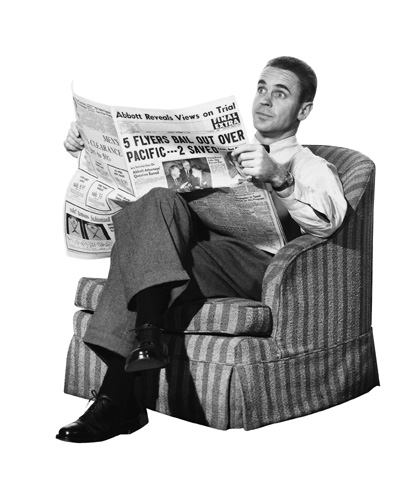
\includegraphics[width=2cm]{img/reading-the-newspaper} \\ \medskip % Picture

%\mySubtitle \\ \medskip % Thesis subtitle
%\myDegree \\
\myDepartment \\
%\myFaculty \\
\myUni \\ \bigskip

\myTime%\ -- \myVersion % Time and version

\vfill

\end{center}
\end{addmargin}

\end{titlepage} % Main title page

%!TEX root = ../thesis.tex
% Back of the title page

\thispagestyle{empty}

\hfill

\vfill

\noindent\myName: \textit{\myTitle,} %\mySubtitle, %\myDegree, 
\textcopyright\ \myTime\\
IMM-MSc-\thesisyear-\thesisnumber

% You may wish to do something with the back of the title page, such as including your supervisors, location or time frame of the work. Below is an example of doing so although you may want to tweak it to your liking.

\bigskip

\noindent\spacedlowsmallcaps{Supervisors}: \\
%\myProf \\
%\myOtherProf \\ 
\mySupervisor \\
\myOtherSupervisor

%\medskip \\

%\noindent\spacedlowsmallcaps{Location}: \\
%\myLocation

%\medskip \\

%\noindent\spacedlowsmallcaps{Time Frame}: \\
%\myTime
 % Back of the title page

%\cleardoublepage% Dedication

\thispagestyle{empty}
\refstepcounter{dummy}

\pdfbookmark[1]{Dedication}{Dedication} % Bookmark name visible in a PDF viewer

\vspace*{3cm}

\begin{center}
\emph{Ohana} means family. \\
Family means nobody gets left behind, or forgotten. \\ \medskip
--- Lilo \& Stitch    
\end{center}

\medskip

\begin{center}
Dedicated to the loving memory of Rudolf Miede. \\ \smallskip
1939\,--\,2005
\end{center} % Dedication page

%\cleardoublepage\include{FrontBackmatter/Foreword} % Uncomment and create a Foreword.tex to include a foreword

\cleardoublepage%!TEX root = ../thesis.tex
% Abstract
\pdfbookmark{Abstract}{Abstract}
\begingroup
\let\clearpage\relax
\let\cleardoublepage\relax
\let\cleardoublepage\relax

\chapter*{Abstract}
This paper proposes a Constraint Programming (CP) approach to personalise a composition of articles that follows rules of the editorial mix in a digital newspaper. Inspiration from conventional newspapers will be used to express the problem as a Constraint Optimisation Problem and solved using local search for CP taking advantage of both probabilistic and logical approaches. Furthermore, this paper proposes a keyword based solution, using WordNet enrichment of articles in combination with a comparison of entities, to determine the relevance of an article to a user defined topic and similarity between articles. As a by-product of the implementation a library for solving personalisation problems using CP was developed.

\vfill

%\selectlanguage{danish}
\pdfbookmark[1]{Resumé}{Resumé}
\chapter*{Resumé}
Denne afhandling præsenterer Constraint Programming (CP) anvendt til at personalisere sammensætningen af artikler i en digital avis, der følger redaktionelle regler. Med inspiration hentet fra konventionelle aviser bliver de redaktionelle regler udtrykt som et Constraint Optimisation Problem og løst vha. local search teknikker for CP. Dette gør at både probalistiske og logiske fordele bliver udnyttet. Udover dette bliver en keywordbaseret løsning præsenteret til at udregne relevans af de enkelte artikler ift. brugerdefinerede emner, men også artiklerne imellem. Løsningen gør brug af WordNet til at berige artiklerne og en sammenligning af entiteter til den semantiske analyse. Som et bi-produkt af implementeringen blev der udviklet et bibliotek til at løse personaliseringsproblemer vha. CP.

%\selectlanguage{british}

\endgroup			

\vfill

%\pdfbookmark[1]{Abstract}{Abstract} % Bookmark name visible in a PDF viewer
%
%\begingroup
%\let\clearpage\relax
%\let\cleardoublepage\relax
%\let\cleardoublepage\relax
%
%\chapter*{Abstract} % Abstract name
%
%Short summary of the contents\dots
%%\todo[inline]{Til Chris: Tusind tak for hjælpen! :)}
%
%\endgroup			

\vfill % Abstract page
%\cleardoublepage%!TEX root = thesis.tex
% Abstract

\pdfbookmark[1]{Abstract}{Abstract} % Bookmark name visible in a PDF viewer

\begingroup
\let\clearpage\relax
\let\cleardoublepage\relax
\let\cleardoublepage\relax

\chapter*{Abstract} % Abstract name

Short summary of the contents\dots
%The thesis establishes the theory of Constraint Programming (CP) and playlists. It applies techniques of CP, logic and functional programming with a similarity function between music pieces to build an Automatic Playlist Generator. The product of the thesis is a program in SML that generates playlists from a users query of suggestions and bans of songs. The similarity function is build solely on measures in tempo and key, which results in playlists that are somewhat useless. The program lack of measures in timbre, rhythm and melody, but is left open for the implementation of these. The thesis finally concludes that the techniques of CP and local search proves efficient for solving the problem.

\endgroup			

\vfill
 % Abstract page
%\cleardoublepage%!TEX root = thesis.tex
%\chapter{} %{Sammenfatning (Summary in Danish)}

\pdfbookmark[1]{Resum\'e}{Resum\'e} % Bookmark name visible in a PDF viewer

\begingroup
\let\clearpage\relax
\let\cleardoublepage\relax
\let\cleardoublepage\relax

\chapter*{Resum\'e} % Abstract name

Kort resum\'e af indholdet\dots
%Projektet præsenterer den grundlæggende teori bag Constraint Programming (CP) og playlists. Strategien i arbejdet med constraints, logisk og funktionel programmering er anvendt til at opstille en Automatic Playlist Generator, som også benytter sig af en funktion til at sammenligne musiknumre. Produktet af projektet er et program i SML der genererer playlists ud fra forslag og forbud på sange fra et bibliotek. Funktionen til sammenligning er alene baseret på sammenligning imellem tempo og toner (key), som resulterer i forholdsvist ubruglige playlists. Programmet mangler sammenligninger imellem klangfarve (timbre), rytme og melodi, men den dynamiske tilgang gør at det let kan implementeres. Til sidst sluttes af den anvendte CP og local search tilgang viser sig effektiv til at løse problemet.

\endgroup			

\vfill % Abstract page
%\cleardoublepage%!TEX root = ../thesis.tex
%\chapter{} %{Sammenfatning (Summary in Danish)}

\pdfbookmark[1]{Preface}{Preface} % Bookmark name visible in a PDF viewer

\begingroup
\let\clearpage\relax
\let\cleardoublepage\relax
\let\cleardoublepage\relax

\chapter*{Preface}
%Time spent on assembling playlists for certain purposes often exceeds the actual use. Some automatic playlist generation engines already exists, but they often lack the possibility of altering the generated playlist - or the option of specifying the length. The result is a repeated query for a playlist until one satisfies and another when it runs out of songs to play.
%
%This thesis is the product of a personal need for an Automatic Playlist Generator.
%
%The thesis is produced under the Department of Informatics and Mathematical Modelling at the Technical University of Denmark and it will presume some knowledge of logic programming and functional programming as it will include an implementation of a program in each language. The preconditions for the thesis are the courses 02156 Formal Logical Systems and 02157 Functional programming taught at the Technical University of Denmark.

\vspace{20mm}
\mbox{}\hfill
\begin{minipage}[t]{80mm}
  Kgs. Lyngby, \myDate
  \\ \\
  \mbox{} \hspace{-16mm} 
\includegraphics{img/signature.eps}
  \myName
\end{minipage}

\endgroup			

\vfill
 % Abstract page
%\cleardoublepage%!TEX root = ../thesis.tex
% Acknowledgements

\pdfbookmark[1]{Acknowledgements}{Acknowledgements} % Bookmark name visible in a PDF viewer

\begin{flushright}{\slshape    
We have seen that computer programming is an art, \\ 
because it applies accumulated knowledge to the world, \\ 
because it requires skill and ingenuity, and especially \\
because it produces objects of beauty.} \\ \medskip
--- \defcitealias{knuth:1974}{Donald E. Knuth}\citetalias{knuth:1974} \citep{knuth:1974}
\end{flushright}

\bigskip

%----------------------------------------------------------------------------------------

\begingroup

\let\clearpage\relax
\let\cleardoublepage\relax
\let\cleardoublepage\relax

\chapter*{Acknowledgements} % Acknowledgements section text

\noindent I would like to thank my family and friends for support and review of the thesis. I would also like to thank my counsellors, Michael Kai Petersen and Carsten Witt from the Department of Informatics and Mathematical Modelling at the Technical University of Denmark, for giving me room for my own definition of the thesis. Also for review of the process and guidance in the right direction.

\endgroup
 % Acknowledgements page

%\cleardoublepage% Publications - a page listing research articles written using content in the thesis

\pdfbookmark[1]{Publications}{Publications} % Bookmark name visible in a PDF viewer

\chapter*{Publications} % Publications page text

Some ideas and figures have appeared previously in the following publications:

\bigskip

\noindent Put your publications from the thesis here. The packages \texttt{multibib} or \texttt{bibtopic} etc. can be used to handle multiple different bibliographies in your document. % Publications from the thesis page

\pagestyle{scrheadings} % Show chapter titles as headings

\cleardoublepage% Table of Contents - List of Tables/Figures/Listings and Acronyms

\refstepcounter{dummy}

\pdfbookmark[1]{\contentsname}{tableofcontents} % Bookmark name visible in a PDF viewer

\setcounter{tocdepth}{2} % Depth of sections to include in the table of contents - currently up to subsections

\setcounter{secnumdepth}{3} % Depth of sections to number in the text itself - currently up to subsubsections

\manualmark
\markboth{\spacedlowsmallcaps{\contentsname}}{\spacedlowsmallcaps{\contentsname}}
\tableofcontents 
\automark[section]{chapter}
\renewcommand{\chaptermark}[1]{\markboth{\spacedlowsmallcaps{#1}}{\spacedlowsmallcaps{#1}}}
\renewcommand{\sectionmark}[1]{\markright{\thesection\enspace\spacedlowsmallcaps{#1}}}

\clearpage

\begingroup 
\let\clearpage\relax
\let\cleardoublepage\relax
\let\cleardoublepage\relax

%----------------------------------------------------------------------------------------
%	List of Figures
%----------------------------------------------------------------------------------------
%
%\refstepcounter{dummy}
%%\addcontentsline{toc}{chapter}{\listfigurename} % Uncomment if you would like the list of figures to appear in the table of contents
%\pdfbookmark[1]{\listfigurename}{lof} % Bookmark name visible in a PDF viewer
%
%\listoffigures
%
%\vspace*{8ex}
%\newpage
%
%%----------------------------------------------------------------------------------------
%%	List of Tables
%%----------------------------------------------------------------------------------------
%
%\refstepcounter{dummy}
%%\addcontentsline{toc}{chapter}{\listtablename} % Uncomment if you would like the list of tables to appear in the table of contents
%\pdfbookmark[1]{\listtablename}{lot} % Bookmark name visible in a PDF viewer
%
%\listoftables
%        
%\vspace*{8ex}
%\newpage
%    
%%----------------------------------------------------------------------------------------
%%	List of Listings
%%---------------------------------------------------------------------------------------- 
%
%\refstepcounter{dummy}
%%\addcontentsline{toc}{chapter}{\lstlistlistingname} % Uncomment if you would like the list of listings to appear in the table of contents
%\pdfbookmark[1]{\lstlistlistingname}{lol} % Bookmark name visible in a PDF viewer
%
%\lstlistoflistings 
%
%\vspace*{8ex}
%\newpage
       
%----------------------------------------------------------------------------------------
%	Acronyms
%----------------------------------------------------------------------------------------

\refstepcounter{dummy}
%\addcontentsline{toc}{chapter}{Acronyms} % Uncomment if you would like the acronyms to appear in the table of contents
\pdfbookmark[1]{Acronyms}{acronyms} % Bookmark name visible in a PDF viewer

\markboth{\spacedlowsmallcaps{Acronyms}}{\spacedlowsmallcaps{Acronyms}}

\chapter*{Acronyms}

\begin{acronym}[UML]
\acro{DRY}{Don't Repeat Yourself}
\acro{API}{Application Programming Interface}
\acro{UML}{Unified Modeling Language}
\end{acronym}  
                   
\endgroup

\cleardoublepage % Contents, list of figures/tables/listings and acronyms

\pagenumbering{arabic} % Arabic page numbering for thesis content (1, 2, 3, etc)
%\setcounter{page}{90} % Uncomment to manually start the page counter at an arbitrary value (for example if you wish to count the pre-content pages in the page count)

\cleardoublepage % Avoids problems with pdfbookmark

%----------------------------------------------------------------------------------------
%	THESIS CONTENT - CHAPTERS
%----------------------------------------------------------------------------------------


\ctparttext{Text for part 1.} % Text on the Part 1 page describing  the content in Part 1

\part{Exploring the field} % First part of the thesis


%%!TEX root = ClassicThesis.tex
% Chapter 1

\chapter{Introduction} % Chapter title

\label{ch:introduction} % For referencing the chapter elsewhere, use \autoref{ch:introduction} 

%----------------------------------------------------------------------------------------

This template for \LaTeX\ has two goals:
\begin{enumerate}
\item Provide students with an easy-to-use template for their Master's or PhD thesis (though it might also be used by other types of authors for reports, books, etc.).
\item Provide a classic, high-quality typographic style that is inspired by \citeauthor{bringhurst:2002}'s ``\emph{The Elements of Typographic Style}'' \citep{bringhurst:2002}.
\marginpar{\myTitle}%\myVersion}
\end{enumerate}

The bundle is configured to run with a \emph{full} MiK\TeX\ or \TeX Live installation right away and, therefore, it uses only freely available fonts.

People interested only in the nice style and not the whole bundle can now use the style stand-alone via the file \texttt{classicthesis.sty}. This works now also with ``plain'' \LaTeX.

As of version 3.0, \texttt{classicthesis} can also be easily used with \mLyX\footnote{\url{http://www.lyx.org}} thanks to Nicholas Mariette and Ivo Pletikosi\'c. The \mLyX\ version of this manual will contain more information on the details.

This should enable anyone with a basic knowledge of \LaTeXe\ or \mLyX\ to produce beautiful documents without too much effort. In the end, this is my overall goal: more beautiful documents, especially theses, as I am tired of seeing so many ugly ones.

The whole template and the used style is released under the \textsmaller{GNU} General Public License. 

If you like the style then I would appreciate a postcard:
\begin{center}
Andr� Miede \\
Detmolder Stra�e 32 \\
31737 Rinteln \\
Germany
\end{center}

\noindent The postcards I received so far are available at:
\begin{center}
 \url{http://postcards.miede.de}
\end{center}
\marginpar{A well-balanced line width improves the legibility of the text. That's what typography is all about, right?} So far, many theses, some books, and several other publications have been typeset successfully with it. If you are interested in some typographic details behind it, enjoy Robert Bringhurst's wonderful book. % \citep{bringhurst:2002}.

\paragraph{Important Note:} Some things of this style might look unusual at first glance, many people feel so in the beginning. However, all things are intentionally designed to be as they are, especially these:
\begin{itemize}
\item No bold fonts are used. Italics or spaced small caps do the job quite well.
\item The size of the text body is intentionally shaped like it is. It supports both legibility and allows a reasonable amount of information to be on a page. And, no: the lines are not too short.
\item The tables intentionally do not use vertical or double rules. See the documentation for the \texttt{booktabs} package for a nice discussion of this topic.\footnote{To be found online at \\ \url{http://www.ctan.org/tex-archive/macros/latex/contrib/booktabs/}.}
\item And last but not least, to provide the reader with a way easier access to page numbers in the table of contents, the page numbers are right behind the titles. Yes, they are \emph{not} neatly aligned at the right side and they are \emph{not} connected with dots that help the eye to bridge a distance that is not necessary. If you are still not convinced: is your reader interested in the page number or does she want to sum the numbers up?
\end{itemize}

\noindent Therefore, please do not break the beauty of the style by changing these things unless you really know what you are doing! Please.

%----------------------------------------------------------------------------------------

\section{Organization}
A very important factor for successful thesis writing is the organization of the material. This template suggests a structure as the following:
\begin{itemize}
\marginpar{You can use these margins for summaries of the text body\dots}
\item\texttt{Chapters/} is where all the ``real'' content goes in separate files such as \texttt{Chapter01.tex} etc.
\item\texttt{FrontBackMatter/} is where all the stuff goes that surrounds the ``real'' content, such as the acknowledgments, dedication, etc.
\item\texttt{img/} is where you put all the graphics you use in the thesis. Maybe they should be organized into subfolders depending on the chapter they are used in, if you have a lot of graphics.
\item\texttt{Bibliography.bib}: the Bib\TeX\ database to organize all the references you might want to cite.
\item\texttt{classicthesis.sty}: the style definition to get this awesome look and feel. Bonus: works with both \LaTeX\ and \textsc{pdf}\LaTeX\dots and \mLyX.
\item\texttt{ClassicThesis.tcp} a \TeX nicCenter project file. Great tool and it's free!
\item\texttt{ClassicThesis.tex}: the main file of your thesis where all the content gets bundled together.
\item\texttt{classicthesis-config.tex}: a central place to load all nifty packages that are used. In there, you can also activate backrefs in order to have information in the bibliography about where a source was cited in the text (\ie, the page number).
    
\emph{Make your changes and adjustments here.} This means that you specify here the options you want to load \texttt{classicthesis.sty} with. You also adjust the title of your thesis, your name, and all similar information here. Refer to \autoref{sec:custom} for more information.

This had to change as of version 3.0 in order to enable an easy transition from the ``basic'' style to \mLyX.
\end{itemize}

\noindent In total, this should get you started in no time.

%----------------------------------------------------------------------------------------

\section{Style Options}\label{sec:options}

There are a couple of options for \texttt{classicthesis.sty} that allow for a bit of freedom concerning the layout: \marginpar{\dots or your supervisor might use the margins for some comments of her own while reading.}
\begin{itemize}
\item General:
\begin{itemize}
\item\texttt{drafting}: prints the date and time at the bottom of each page, so you always know which version you are dealing with. Might come in handy not to give your Prof. that old draft.
\end{itemize}
	
\item Parts and Chapters:
\begin{itemize}
\item\texttt{parts}: if you use Part divisions for your document, you should choose this option. (Cannot be used together with \texttt{nochapters}.)

\item\texttt{nochapters}: allows to use the look-and-feel with classes that do not use chapters, \eg, for articles. Automatically turns off a couple of other options: \texttt{eulerchapternumbers}, \texttt{linedheaders}, \texttt{listsseparated}, and \texttt{parts}. 

\item\texttt{linedheaders}: changes the look of the chapter headings a bit by adding a horizontal line above the chapter title. The chapter number will also be moved to the top of the page, above the chapter title.
\end{itemize}

\item Typography:
\begin{itemize}
\item\texttt{eulerchapternumbers}: use figures from Hermann Zapf's Euler math font for the chapter numbers. By default, old style figures from the Palatino font are used.

\item\texttt{beramono}: loads Bera Mono as typewriter font. (Default setting is using the standard CM typewriter font.)
\item\texttt{eulermath}: loads the awesome Euler fonts for math. (Palatino is used as default font.)

\item\texttt{pdfspacing}: makes use of pdftex' letter spacing capabilities via the \texttt{microtype} package.\footnote{Use \texttt{microtype}'s \texttt{DVIoutput} option to generate DVI with pdftex.} This fixes some serious issues regarding math formul\ae\ etc. (\eg, ``\ss'') in headers. 

\item\texttt{minionprospacing}: uses the internal \texttt{textssc} command of the \texttt{MinionPro} package for letter spacing. This automatically enables the \texttt{minionpro} option and overrides the \texttt{pdfspacing} option.
\end{itemize}  

\item Table of Contents:
\begin{itemize}
\item\texttt{tocaligned}: aligns the whole table of contents on the left side. Some people like that, some don't.

\item\texttt{dottedtoc}: sets pagenumbers flushed right in the table of contents.

\item\texttt{manychapters}: if you need more than nine chapters for your document, you might not be happy with the spacing between the chapter number and the chapter title in the Table of Contents. This option allows for additional space in this context. However, it does not look as ``perfect'' if you use \verb|\parts| for structuring your document.
\end{itemize}

\item Floats:
\begin{itemize}
\item\texttt{listings}: loads the \texttt{listings} package (if not already done) and configures the List of Listings accordingly.
    
\item\texttt{floatperchapter}: activates numbering per chapter for all floats such as figures, tables, and listings (if used).	
    
\item\texttt{subfig}(\texttt{ure}): is passed to the \texttt{tocloft} package to enable compatibility with the \texttt{subfig}(\texttt{ure}) package. Use this option if you want use classicthesis with the \texttt{subfig} package.

\end{itemize}    

\end{itemize}

\noindent The best way to figure these options out is to try the different possibilities and see, what you and your supervisor like best.

In order to make things easier in general, \texttt{classicthesis-config.tex} contains some useful commands that might help you.

%----------------------------------------------------------------------------------------

\section{Customization}\label{sec:custom}

This section will give you some hints about how to adapt \texttt{classicthesis} to your needs.

The file \texttt{classicthesis.sty} contains the core functionality of the style and in most cases will be left intact, whereas the file \texttt{classic\-thesis-config.tex} is used for some common user customizations. 

The first customization you are about to make is to alter the document title, author name, and other thesis details. In order to do this, replace the data in the following lines of \texttt{classicthesis-config.tex:}\marginpar{Modifications in \texttt{classic\-thesis-config.tex}
}

\begin{lstlisting}[frame=lt]
\newcommand{\myTitle}{A Classic Thesis Style\xspace}
\newcommand{\mySubtitle}{An Homage to ...\xspace}
\newcommand{\myDegree}{Doktor-Ingenieur (Dr.-Ing.)\xspace}
\end{lstlisting}

Further customization can be made in \texttt{classicthesis-config.tex} by choosing the options to \texttt{classicthesis.sty} (see~\autoref{sec:options}) in a line that looks like this:

\begin{lstlisting}[frame=lt]
\PassOptionsToPackage{eulerchapternumbers,listings,drafting, pdfspacing, subfig,beramono,eulermath,parts}{classicthesis}

\end{lstlisting}

If you want to use backreferences from your citations to the pages they were cited on, change the following line from:
\begin{lstlisting}[breaklines=false,frame=lt]
\setboolean{enable-backrefs}{false}
\end{lstlisting}
to
\begin{lstlisting}[breaklines=false,frame=lt]
\setboolean{enable-backrefs}{true}
\end{lstlisting}

Many other customizations in \texttt{classicthesis-config.tex} are possible, but you should be careful making changes there, since some changes could cause errors.

Finally, changes can be made in the file \texttt{classicthesis.sty}, \marginpar{Modifications in \texttt{classicthesis.sty}} although this is mostly not designed for user customization. The main change that might be made here is the text-block size, for example, to get longer lines of text.

%----------------------------------------------------------------------------------------

\section{Issues}\label{sec:issues}
This section will list some information about problems using \texttt{classic\-thesis} in general or using it with other packages.

Beta versions of \texttt{classicthesis} can be found at the following Google code repository:
\begin{center}
\url{http://code.google.com/p/classicthesis/}
\end{center}

\noindent There, you can also post serious bugs and problems you encounter.

\subsection*{Compatibility with the \texttt{glossaries} Package}
If you want to use the \texttt{glossaries} package, take care of loading it with the following options:
\begin{verbatim}
\usepackage[style=long,nolist]{glossaries}
\end{verbatim}

\noindent Thanks to Sven Staehs for this information. 

\subsection*{Compatibility with the (Spanish) \texttt{babel} Package}
Spanish languages need an extra option in order to work with this template:
\begin{verbatim}
\usepackage[spanish,es-lcroman]{babel}
\end{verbatim}

\noindent Thanks to an unknown person for this information (via Google Code issue reporting). 

\subsection*{Compatibility with the \texttt{pdfsync} Package}
Using the \texttt{pdfsync} package leads to linebreaking problems with the \texttt{graffito} command. Thanks to Henrik Schumacher for this information. 

%----------------------------------------------------------------------------------------

\section{Future Work}
So far, this is a quite stable version that served a couple of people well during their thesis time. However, some things are still not as they should be. Proper documentation in the standard format is still missing. In the long run, the style should probably be published separately, with the template bundle being only an application of the style. Alas, there is no time for that at the moment\dots it could be a nice task for a small group of \LaTeX nicians.

Please do not send me email with questions concerning \LaTeX\ or the template, as I do not have time for an answer. But if you have comments, suggestions, or improvements for the style or the template in general, do not hesitate to write them on that postcard of yours.

%----------------------------------------------------------------------------------------

\section{License}
\paragraph{GNU General Public License:} This program is free software; you can redistribute it and/or modify it under the terms of the \textsmaller{GNU} General Public License as published by the Free Software Foundation; either version 2 of the License, or (at your option) any later version.

This program is distributed in the hope that it will be useful, but \emph{without any warranty}; without even the implied warranty of \emph{merchantability} or \emph{fitness for a particular purpose}. See the \textsmaller{GNU} General Public License for more details. % Chapter 1

%!TEX root = ../thesis.tex
\chapter{Creating the Editorial Mix} % (fold)
\label{ch:introduction}
This chapter introduces the editorial mix of a digital newspaper and which parameters to account for when composing the newspaper. It is afterwards discussed which of these parameters are suited for personalisation, and how this can be done. The proposed approach is then presented with its pros and cons, which results in a list of contributions this project has to the field of personalisation.
%\todo[inline]{Introduce an automated editorial mix to the digital newspaper. Bringing rss-readers and digital newspapers closer together.}

\section{What is the Editorial Mix}
In the conventional newspapers the editors job is to compose an intriguing front page that offers the contents of the sections that might interest the individual user. His challenge is to accommodate the needs of the newspapers segment of readers, divide the articles into sections, with a nice reading flow and attractive illustrations, and hand-pick articles to go on the front page. But what if a computer could do this?
%"their segment of readers", hvis readers? Måske det ville lyde bedre hvis man skrev "the paper's segment of readers" eller noget i den dur.

\cite{perkowitz-Adaptive-Web-Sites} decomposes the problem of synthesising adapted page into several subproblems\sidenote{In the subproblems stated here, ``hyperlink'' has been replaced by ``item'' to appreciate them more generally, rather than the original specific sense.}:
\begin{itemize}
	\item What is the content (that is, set of items) of the index page?
	\item Does it have a coherent topic? What should its title be?
	\item How are the items on the page ordered?
	\item How are the items labeled?
	\item Is the page consistent with the site's overall graphical style?
	\item Is it appropriate to add the page to the site? If so, where?
\end{itemize}

Some efforts have been made to digitally calculate similarities between articles and based on a current article suggest similar reading material or use collaborate filtering to suggest articles based on other users reading behaviour. Some papers proposes a composition of articles from user picked RSS-feeds, which can, e.g.\ in the case of Google Reader, be divided into sections. This comes close to conventional newspapers, but there is no ordering of the flow of articles. The ordering, flow and choice of relevant articles is here on referred to as the \emph{relational} part of the editorial mix.
% "Others offer composition of articles..." Others giver ikke mening her, hvem mener du?

The solution for some digital newspapers are still to have an editor to create their coherent composed digital newspaper, like the New York Times or Wired Magazine. Flipboard, on the other hand, composes their editorial mix of articles from feeds and divides their pages  into three or more rarely four or five articles\sidenote{Flipboard includes specialised layouts with more articles per page for Twitter.} with excerpts and images, much like conventional newspapers front pages. How they choose their composition is kept a business secret, but it does seem to vary a lot, see Figure~\ref{fig:flipboard-screenshot}.

\begin{figure}[h!tb]
 	\begin{center}
 		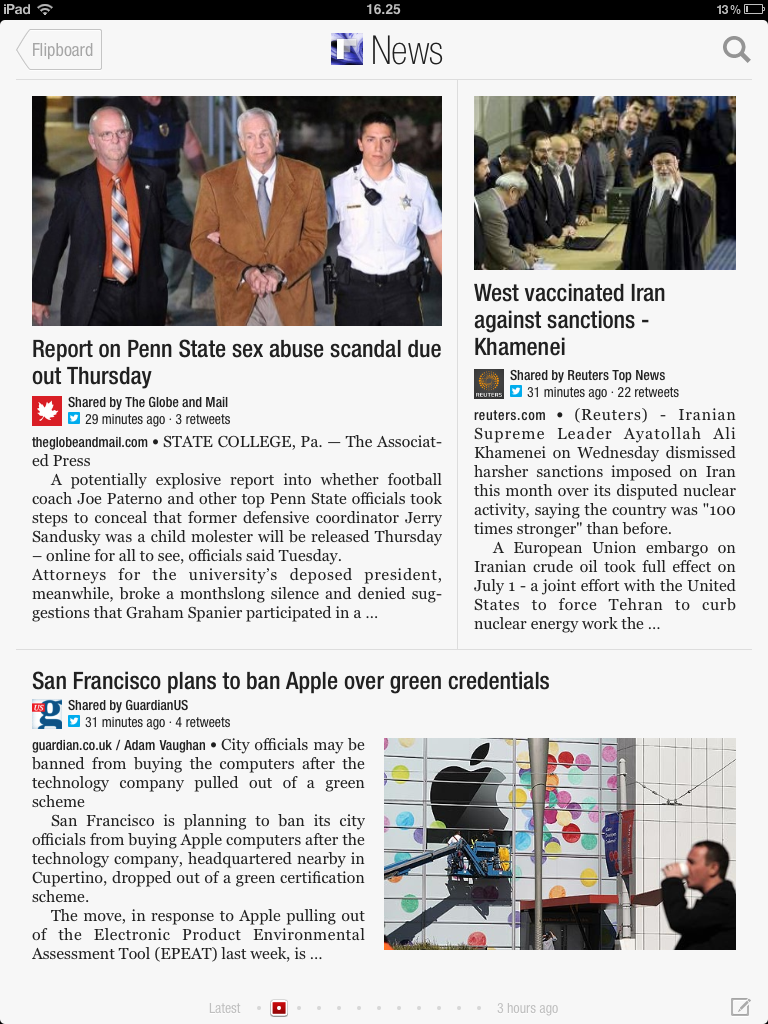
\includegraphics[width=.45\textwidth]{img/flipboard2}
 	\end{center}
 	\caption{A screenshot of composition of three articles in Flipboard, with different subjects, i.e.\ world crime, world finance and technology news.}
 	\label{fig:flipboard-screenshot}
\end{figure}

\todo[inline]{Maybe put in a reference to a conventional newspaper.}

It is hard to say if there is a control behind the placement of content other than the choice of featured and non-featured articles, but this is actually an example of a computationally composed newspaper. The placement and amount of room given for an article is here on referred to as the \emph{spacial} part of the editorial mix.

Finally, subjects of articles have more relevance at some points in time than others and editors choose the amount of time stories should be available in, where RSS-readers just displays the newest articles first, which are not always the most relevant. This selection of articles within a chosen time frame is here on referred to as the \emph{temporal} part of the editorial mix.

One thing that is vastly different from newspapers to RSS-readers is the ability to deliver personalised content, in that a user can choose which RSS-feeds to follow, whereas readers of newspapers need to navigate it in order to find interesting articles. Also where newspapers have quality assurance of its content, RSS-readers have a seemingly unlimited amount of articles.

\section{Personalising a Digital Newspaper}
\cite{BushMemex} describes a collective memory library machine that can be indexed, called the memex. Items in the library are linked together forming personal association trails. This is the early conception of the hypertext media that would later become the World Wide Web and later personalised web applications. With many respects that is what this project tries to achieve; i.e.\ link information in the form of articles together and present them in personalised trials defined by the user. As opposed to \cite{BushMemex} proposed manual linking it is now possible to, e.g.\ classify and compute similarity automatically, which greatly aids the process. 

User preferences are very diverse and it is therefore hard to accommodate every individual in a single solution. A digital solution must be bound to a specific domain, but must also be open for novel use.

%\begin{quotation}
%	``Web personalization is the process of customizing a Web site to the needs of specific users, taking advantage of the knowledge acquired from the analysis of the user's navigational behavior (usage data) in correlation with other information collected in the Web context, namely, structure, content, and user profile data.'' \cite{MagdaliniWebMining}
%\end{quotation}
\begin{minipage}{.8\largefigure}
\begin{flushleft}{\slshape
``Web personalization is defined as any action that adapts the information or services provided by a Web site to the needs of a particular user or a set of users, taking advantage of the knowledge gained from the users' navigational behavior and individual interests, in combination with the content and the structure of the Web site.''} \\ \medskip
-- \cite{MagdaliniWebMining}
\end{flushleft}
\end{minipage}
	
%\cite{WebMiningMulvenna} defines the goal of personalisation systems as follows: ``to provide users with the information they want or need, without expecting from them to ask for it explicitly''

The three categories of the editorial mix can be described in the sense of personalisation as well. Accommodating user preference based on spacial personalisation is achieved by a placement of articles, temporal personalisation by selecting articles of higher news value based on their relevance time frame and finally, relational personalisation by selecting articles that provides more value based on their respective and collaborate topics. Temporal personalisation is also obtained by letting user preferences have a life time and decrease the preference influence on which articles to select as time passes.
%Der er noget galt her, men er ikke helt sikker på hvad: "decrease its in influence.."

All three categories are related as they each provide some value to the editorial mix, e.g.\ a different spacial placement of a specific article can provide a different composition of the editorial mix and therefore a different temporal and/or relational value to the user.
%or the editorial composition/arrangement

\section{Contributions of Constraint Programming}
\hspace{-\marginparwidth}
\begin{minipage}{.8\largefigure}
\begin{flushright}{\slshape
	``Informally, declarative programming involves stating \emph{what} is computed, but not necessarily \emph{how} it is computed. Equivalently, in the terminology of Kowalski's equation $algorithm = logic + control$, it involves stating the \emph{logic} of an algorithm, but not necessarily the \emph{control}.''} \\ \medskip
-- \cite{LloydDeclarative}
\end{flushright}
\end{minipage}
%
%\begin{quotation}
%``The logic component determines the meaning of the algorithm whereas the control component only affects its efficiency [...] When logic is separated from control, it is possible to distinguish (in the logic) what the program does from how the program does it (in the control)'' \cite{KowalskiAlgo}
%\end{quotation}

As a declarative programming language, Constraint Programming (CP) offers means for describing the problem to be solved using constraints and a general purpose constraint solver. Once the general purpose solver is set up, the constraints can be defined to model the problem to be solved, but does not necessarily make it easy. However, the problem definition can easily be extended and/or modified afterwards.

\hspace{-\marginparwidth}
\begin{minipage}{.8\largefigure}
\begin{flushright}{\slshape
	``Ordinary people generally aren't interested (and rightly so) in low-level programming details -- they just want to express the problem in some reasonably congenial way and let the system get on with solving the problem. [...] Having to deal only (or mostly) with the logic component simplifies many things for the programmer. First, (the logic component of) a declarative program is generally easier to write and to understand than a corresponding imperative program. Second, a declarative program is also easier to reason about and to transform, as much current research in functional and logic programming shows.''} \\ \medskip
-- \cite{LloydDeclarative}
\end{flushright}
\end{minipage}

Also, with logic comes precise solutions, but this does not come without a cost as stochastic approaches often beat logic by lengths. However, stochastic variables can be introduced to CP.

%\section{Short Introduction to Constraint Programming}
%\label{sec:CP}
To be able to work with personalisation problems as Constraint Satisfaction Problems (CSPs) or Constraint Optimisation Problems (COPs), these need to be defined. The following descriptions of CSPs and COPs have been modified to fit personalisation problems from the original definitions provided by \cite{AIRussell} and~\cite{CPApt}.

A Constraint Satisfaction Problem is defined by the 3-tuple $(\mathcal{X}, \mathcal{D}, \mathcal{C})$, where $\mathcal{X}$ is the set of variables, $\mathcal{D}$ is the corresponding set of domains and $\mathcal{C}$ is the set of constraints on the variables.

Each variable has sub-domains corresponding to the sub-value of each value. And unlike \cite{AIRussell} and~\cite{CPApt} a constraint is here defined as a function of specific variables returning a boolean value. Therefore the tuple of $n$ variables with $m$ sub-variables and $k$ constraints on $r$ and $s$ number of variables, respectively, can be expanded to:

\begin{align*}
\begin{pmatrix}\vspace{3pt}
	\mathcal{X} :
	\begin{Bmatrix}
		x_1 :
		\begin{pmatrix}
			x_1.a_1\\
			\ldots\\
			x_1.a_m\\
		\end{pmatrix}
		, \cdots,
		x_n :
		\begin{pmatrix}
			x_n.a_1\\
			\ldots\\
			x_n.a_m\\
		\end{pmatrix}
	\end{Bmatrix},\\\vspace{1pt}
	\mathcal{D} :
	\begin{Bmatrix}
		d_1 :
		\begin{pmatrix}
			d_1.a_1\\
			\ldots\\
			d_1.a_m\\
		\end{pmatrix}
		, \cdots,
		d_n :
		\begin{pmatrix}
			d_n.a_1\\
			\ldots\\
			d_n.a_m\\
		\end{pmatrix}
	\end{Bmatrix},\\\hspace{3pt}
	\mathcal{C} :
	\begin{Bmatrix}
		c_1 : func(x_i, \cdots,x_{i+r}) \rightarrow \mathbb{B}, \cdots, c_k : func(x_j, \cdots,x_{j+s}) \rightarrow \mathbb{B}
	\end{Bmatrix}\hspace{3pt}
\end{pmatrix}
\end{align*}
Where $\mathbb{B}$ is either \texttt{true} or \texttt{false}.

A CSP is a subset of a Constraint Optimisation Problem (COP) and a COP is defined by the 4-tuple $(\mathcal{X}, \mathcal{D}, \mathcal{C}, \mathcal{O})$, where the three first elements are defined as in a CSP and $\mathcal{O}$ is a set objective (or cost) functions on variables, that determines the quality of a current state. The set of objective functions can be described with the same structure as constraints in CSPs and can be expanded as follows with $l$ number of functions on $t$ and $u$ number of variables, respectively.

\begin{align*}
	\mathcal{O} :
	\begin{Bmatrix}
		o_1 : func(x_i, \cdots,x_{i+t}) \rightarrow \mathbb{R}, \cdots, o_l : func(x_j, \cdots,x_{j+u}) \rightarrow \mathbb{R}
	\end{Bmatrix}
\end{align*}

Where $\mathbb{R}$ is the set of real numbers.

Satisfaction (or regular) constraints are also called hard constraints and objective functions, soft constraints because a solution can be found if all hard constraints are satisfied, whereas and optimal assignment is enough to satisfy objective functions.
%\subsection{Constraint Optimisation Problems}
%Wiki: ``A constraint optimization problem can be defined as a regular constraint satisfaction problem in which constraints are weighted and the goal is to find a solution maximizing the weight of satisfied constraints.
%Alternatively, a constraint optimization problem can be defined as a regular constraint satisfaction problem augmented with a number of `local' cost functions. The aim of constraint optimization is to find a solution to the problem whose cost, evaluated as the sum of the cost functions, is maximized or minimized.''
%\todo[inline]{Find reference that is not from wikipedia}

%\todo[inline]{? Første side er vigtig for karaktergivningen. ``Det er komplekst det her, Nå, der er et bud på det... osv.''}
%\todo[inline]{Introduce web personalisation}
\section{Problem Description}
This project is a feasibility study of the implementation of CP in the field of personalisation. The criteria of success is whether it is possible to successfully implement the techniques of personalisation using CP and to make personalisation more accessible with the aid of CP.
%\footnote{In constraint satisfaction, constrained optimization seeks for a solution maximizing or minimizing a cost function, Wikipedia.}
%\footnote{Personalization involves using technology to accommodate the differences between individuals, Wikipedia.}
%The overall idea is to implement CP as a technique for personalisation of digital solutions and attempt to make personalisation more accessible with the aid of CP.
Therefore the project will be divided into two main areas; i.e.\ the an assessment of the use of CP in the context of personalisation and a direct application of this in the form of a personal digital newspaper, where CP is used to personalise the content and composition of a digital newspaper.

Many techniques for personalising digital solutions already exists, but the role of CP within this domain has not been determined. This project seeks to explore CP as a tool to make the personalisation of digital solutions more accessible.

\subsection{Personalisation Challenges}
In an attempt to introduce a personal editorial mix in the digital newspaper, the report will try to analyse which preferences the users will have with respect to the content, composition and the time frame of relevant articles. It will describe the search for articles to fit the user needs as an Constraint Optimisation Problem and try to solve it. What makes a newspaper is not only the accumulated content of its articles, but the arrangement of them. ``Which articles should go where'' is just as important, and the placement of articles in the newspaper should therefore go through an equal solving process.

\subsection{Algorithmic Challenges}
To be able to use and assess CP in the context of personalisation a full understanding must be acquired. Features that can be solved using CP will be modelled as a COP and solved. Furthermore, because the problem has a fixed budget for finding a solution, its algorithmic complexity will be analysed. The findings will be concluded in an evaluation of the applicability of CP to personalisation problems.

%
%
%
%\subsection{Subproblem specification}
%Before evaluating the use of COPs with respect to personalisation it needs to be determined whether the problem can actually be described as a COP. Moreover, the editorial constraints needs to be defined. These will constitute a knowledge base of ground rules from which a paper will be generated. The article will look into current media, i.e.\ radio programmes, television programmes, magazines and of cause news papers, to try to specify rules of layout and succession of articles based on metadata. The first part of this article will address this problem.
%
%A crucial part of the project is also to lay down the means of bringing content to the paper. A normal way to do this would be to use feeds or to scrape web sites (extracting information from web sites) of articles. The pros and cons of each method and further options needs to be addressed and an optimal solution chosen. This will constitute the second part of the article.
%
%
%
%
%bedste måde at inddrive den information vi skal bruge for at kunne arbejde med det og generere den digitale avis der passer dig bedst
%
%analyse -- cop i dybden medier kan -- synagien i et layout genskabes fra links og tweets?, design, implementation -- web, anvende, test (evaluere). Realtion til playlist -- som går på at få en stemning kommunikeret. Bygge en oplevelse -- hver artikel bidrager til helheden. tværsnit. analyse=model+brugerpræferencer. topic (flere) vs. genre (én). grænseværdi for topics (hvor mange giver mening) granulalitet. genre i første omgang. analysere sig frem til sammensætning af ord => definere topics -- distributioner af ord. mappe ord fra topic knowledge base til artikel. opbygge og glemme viden gradvist (1 måned eller 1 år?). Udvælge punkter der kunne være at undersøge.
%
%
%%%%%%%%%%%%%%%%%%%%% Initial problem specification %%%%%%%%%%%%%%%%%%%%%%%%%
% Optimising the Editorial Mix for a Digital Newspaper using Constraint Programming
% Optimering af den Redaktionelle Sammensætning i en Digital Avis med brug af Constraint Programmering
% start 6/2
% aflevering 3/8
% General project objectives:
% The overall objective of the project is to make the student familiar with Constraint Programming, especially Constraint Optimised Problems, and its uses in the context of personalisation. A specific personalisation problem is implemented and solved using Constraint Programming and relevant metaheuristics. Finally, the project provides a conceptual basis for developing personal digital solutions and the uses for Constraint Programming.
% Learning objectives:
% Explore existing literature and summarise it.
% Analyse the applicability of personalisation in a given domain and derive features of the problem to be personalised.
% Find applicable metaheuristics for personalisation problems and refine them accordingly.
% Model the identified features as constraints in a Constrained Optimisation Problem. Solve the defined Constraint Optimisation Problem in Constraint Programming.
% Evaluate Constraint Programming as a tool for personalisation problems and compare the solution to existing solutions.
% Describe and discuss the project in a report and present it orally.
%
%
%%%%%%%%%%%%%%%%%%%%%%%%%%%%%%%%%%%%%%%%%%%%%%%%%%%%%%%%%%%%%%%%%%%%%%%%%%%%%%%%%
%\subsection{General Project Objectives}
%The overall objective of the project is to make the student familiar with Constraint Programming, especially Constraint Optimised Problems, and its uses in the context of personalisation. A specific personalisation problem is implemented and solved using Constraint Programming and relevant metaheuristics. Finally, the project provides a conceptual basis for developing personal digital solutions and the uses for Constraint Programming.
%
%\subsection{Learning Objectives}
%Explore existing literature and summarise it.
%Analyse the applicability of personalisation in a given domain and derive features of the problem to be personalised.
%Find applicable metaheuristics for personalisation problems and refine them accordingly.
%Model the identified features as constraints in a Constrained Optimisation Problem.
%Solve the defined Constraint Optimisation Problem in Constraint Programming.
%Evaluate Constraint Programming as a tool for personalisation problems and compare the solution to existing solutions.
%Describe and discuss the project in a report and present it orally.
%
%%%%%%%%%%%%%%%%%%%%% Revised Problem Specification: %%%%%%%%%%%%%%%%%%%%%%%%%%
% Blooms taxonomy:
%knowledge
%comprehension
%application
%analyse
%synthesise
%evaluate
%
%\subsection{Title}
%Personalising the Editorial Mix for a Digital Newspaper using Constraint Programming
%
%\subsection{Danish Title}
%Personalisering af den Redaktionelle Sammensætning i en Digital Avis med brug af Constraint Programmering
%
%\subsection{Time Frame}
%Project start 6/2-2012, delivery 3/8-2012.
%
%\subsection{General Project Objectives}
%The overall objective of the project is to make the student familiar with personalisation and the concept of modelling user preferences in digital solutions. A specific personalisation problem is analysed and relevant design proposals are discussed. A chosen design is implemented and solved using Constraint Programming. The project provides a conceptual basis for the use of Constraint Programming in the context of developing personalised digital solutions. Finally, the project attempts to make personalisation more accessible for developers with the introduction of Constraint Programming to the field.
%
%\subsection{Learning Objectives}
%Explore existing literature and summarise it.
%
%Analyse the applicability of personalisation in a given domain and derive features of the problem to be personalised.
%
%%Identify features in the domain that can be solved using Constraint Programming.
%
%Model the identified features as constraints and solve them using Constraint Programming.
%
%%Refine the identified features into general guidelines for the use of Constraint Programming in the context of personalisation.
%
%%Evaluate Constraint Programming as a tool for personalisation problems and compare the solution to existing solutions.
%
%Evaluate the solution and compare existing techniques for personalisation to the ones used in the solution.%betyder dette også at definere dens plads iblandt?
%
%Describe and discuss the project in a report and present it orally.
%%%%%%%%%%%%%%%%%%%%%%%%%%% end of Revised problem spec %%%%%%%%%%%%%%%%%%%%%%%%%%%%%%%
% section introduction (end)
%!TEX root = ../thesis.tex
\chapter{Perspectives and Inspirations}
\label{ch:related_work}
Web personalisation is by \cite{DataMiningMobasher} divided into phases of data collection and preprocessing, pattern discovery and evaluation, and applying the discovered knowledge in real-time to mediate between the user and the Web. There have been many suggestions on how to tackle these different processes of creating the interactive personalised digital newspaper. \cite{gervasum2001ws.pdf} proposes a strictly stochastic approach to dynamic personalisation obtained by characterisation of content and user's interests. Both implicit and explicit relevance feedback\footnote{Implicit is when the (unaware) user's behaviour is recorded to determine relevance and explicit is where the user is aware of the action of giving the feedback.} is used to refine the user models. Stochastic approaches have the advantage of being effective, but often solves a very specific problem. Also, these approaches tend to get very complex in order to deliver promising results. Some cope with this by introducing logic to the problem like it is done in \cite{SpacialLogicNilsson} with a spacial approach. In this project it is possible to benefit from the structure of the logic approach of CP and the effectiveness of a stochastic approach by introducing preference constraints with an objective function.

\todo[inline]{Reference for stochastic approaches?}

Many uses the approach of computing the tf-idf similarity with a cosine function as the distance function, as it is done in \cite{fulltext.pdf} to apply relational personalisation. It is based on a set of keywords extracted from the news items and a set of training documents. This constitutes the initial approach for computing similarity in this project. However, \cite{10-1-1-19-5583} argues that semantic knowledge is more substantial than keywords. 

Classification techniques can be applied in order to ease the task of selecting relevant articles and determine their mutual relationships. \cite{gervasum2001ws.pdf} uses a library of documents to train a categorisation algorithm and the users are then asked to select categories of which they have interest. \cite{10-1-1-19-5583}, on the other hand uses a thesaurus of hierarchically, and to the task specifically, structured terms to index news articles. Results of the indexing are thereafter mapped with user profiles to select the relevant articles. In stead of using predefined root terms as the basis for a classification, WordNet can be used to obtain semantic knowledge for a document. WordNet is a large lexical database of English words and their relationships in the form of different graphs. \cite{116262780379.pdf} presents an algorithm for enriching articles using WordNet's hypernym-graphs. WordNet also contains similarity functions between words. These functions will later on constitute the next step for computing similarity in this project.

\cite{fulltext.pdf} does present the means of combining the use of categories and keywords, but this approach demands predefined categories, which must be kept updated in order to follow semantic changes to the field. The time limitations and prioritisation of this project did not allow for a thesaurus to be obtained to aid the classification and will therefore not be introduced to the solution. One, could also argue that semantic assumptions are made, when categories are predefined, which could lead to some false classification. Whereas the structure of \cite{116262780379.pdf}'s algorithm bases its semantic structure only on words from the article and the general semantic (and more neutral) structure that constitutes the basis for WordNet.

\cite{10.1.1.45.5230.pdf} presents a combination of content-based and collaborate filters to predict interest in articles based on a user profile.

\cite{10.1.1.45.5230.pdf} presents a front page design and available sections. A section can appear as their front page.
relevance feedback

their editorial mix consists of ordering the articles by most predicted interest first.

\cite{fulltext.pdf} along with both a short- and long-term representation of the user models. Furthermore, a global user profile, to get the process of generating the user model started.

\cite{Personalizing-your-electronic-newspaper.pdf} incorporates temporal personalisation in that it is possible to ask for articles in the newspaper based on a specific period, but also by incorporate ageing of user interests.

\cite{Estebanetal.pdf} incorporates temporal features of their personalisation of a digital newspaper based on Yahoo! Spain. Automatic Categorisation of news items, long- and short-term user models.

In the explored literature users shows much interest in being able to turn pages as it is done in a regular newspaper. \cite{FULLTEXT01.pdf} describes this as ``open, turn pages, chose article, read and return''.

\cite{fulltext.pdf} proposes the use of collaborate filtering to handle the problem of converging, which is what will happen if no non-personalised articles are introduced, but this still only concerns articles that are within the area of the users interest. If e.g.\ a user has not shown interest in politics, the news of Barack Obama becoming the President of USA will never be included in the newspaper. Instead a ratio between personalised and general articles will solve this issue, and since it is not within everyones interest to receive general news, this ratio should be adjustable.

Users navigate the newspaper using sections and headlines as the main entry points \cite{FULLTEXT01.pdf} and these should therefore be kept in the digital version.

Users express that these should be put into menu \cite{kristin_fredrik.pdf}.

\cite{fulltext.pdf} proposes personalised excerpts from the articles to further ease the navigation.

There exist many different examples of preference modelling using CP, and \cite{Constraint-Satisfaction-Methods-for-Information-Personalization.pdf} describes a factual information system to find personal information, e.g.\ about healthcare. They present two constraints: (1) select only information-objects that correspond to the user-model and; (2) the content of the retained information-items do not contradict each other. This is an example of an editorial mix in that it incorporates the relational features, i.e.\ both between user and articles, and articles in between. However, they do not take into account the spacial part of their editorial mix, nor do they take into account any temporal features of the information needed. It is of cause notable that the user needs for a strictly factual information system are different than from a newspaper.

Another application of preference modelling using CP is \cite{LSVossen}. He proposes a CP approach to automatic playlist generation, which very much relates to what this project attempts to achieve. A playlist can be perceived as a, in this case, personal mix of songs. He presents constraints to exclude songs with certain attributes, to model that certain songs should be similar to each other or a user preference, to describe preference about the number of songs from a specific artist and the well-known \texttt{all-diff} constraint. These can be directly translated to the editorial mix of a newspaper, where the songs are articles and artists could be a specific author or content provider.

\todo[inline]{som afslutning på kapitel 2 kunne du opsummere hvilke features du mener er mest relevante så det ikke bare bliver en lang liste}

\todo[inline]{You might also want to combine related work (3) and method (4) since it is easier to explain your own work in relation to the work it is built upon. Just make sure that your own contribution is not hidden. The reader will want to know what you did!}

This paper proposes a Constraint Programming (CP) approach to solve the editorial mix problem. The problem will be expressed as a Constraint Optimisation Problem and solved using local search for CP. Furthermore, this paper proposes a keyword based solution in combination with a comparison of entities for determining the relevance for an article to a user defined topic and similarity between articles.

\todo[inline]{Er der argumenteret for at bruge keywords?}
personalised topics in stead of the generic definition of the terms. Maybe what the crowd thinks is technology is not what you deem as technology

%``Constraint programming (CP) is an emergent software technology for declarative description and effective solving of large, particularly combinatorial, problems especially in areas of planning and scheduling. [...] it is attracting widespread commercial interest as well, in particular, in areas of modelling heterogeneous optimisation and satisfaction problems.'' \cite{RomanCP}
%
%Where CP provides a declarative approach, with the possibility of introducing stochastic variables a purely stochastic approach also has it advantages.
%
%Stochastic approaches like the graph based Hidden Markov Model or the spacial like the one proposed in  are usually very effective, but often at the cost of being imprecise, but logic can also be introduced to stochastic approaches, \cite{SpacialNilsson}.
%\todo[inline]{Find reference for this.}
%
%A graph approach to the problem could be a good solution as fast algorithms have been developed to minimise computation time. An example of this is the Hidden Markov Model which works on a dynamic Bayesian network\footnote{For more information \url{http://en.wikipedia.org/wiki/Hidden_Markov_model}.}. Here attributes or meta data of the article can be 
%
%\todo[inline]{Alternative solutions: graph based (Hidden-Markov-Models) and clustering, spacial distance (references to ConQuest NilssonHaav.pdf and 10 -Concept Spaces.pdf) in n-dimensional space is fast.}
%\todo[inline]{formal logical approach will probably be beaten by stochastic solutions in speed, however they are imprecise. The happy medium is a combination of logical and stochastic approaches. Trade-off: imprecise stochastic/precise logic. To find the balance is very hard.}
%\subsection{Existing solutions}
%Personalisation of digital solutions becomes more common everyday and users demand personalised solution to accommodate their needs.
%!TEX root = ../thesis.tex
\chapter{Features to be Personalised} % (fold)
\label{ch:analysis}
This section analyses the user preferences and identifies which features should be modelled as personalisation constraints. It also seeks to define the default setting that consists the general model for a good editorial mix of a digital newspaper.

The focus of automatically generating the editorial mix introduces temporal, spacial and relational circumstances about the composition. But before these can be modelled as constraints it is necessary to look at the user needs of the application.
%
%These will consist the content constraints of the system along with those determined by user preferences. Therefore the constraints that belongs to composition conditions must be presented/defined.

Also some prerequisites must be stated in order to set the focus of the problem, but also for the potential user to relate to the product. The research done by \cite{FULLTEXT01.pdf} and \cite{kristin_fredrik.pdf} determines the preferable size of the digital newspaper to be $14.732 \times 20.828$cm $\sim$ size A5, which reflects the size of the iPad. Therefore this project will target the iPad as its primary device. The hand-held device also introduces mobility, which is also of great preference to the potential users.
%
%\begin{itemize}
	%\item $14.732 \times 20.828$cm $\sim$ size A5, which reflects the size of the iPad% \cite[p. 1]{FULLTEXT01.pdf} % \cite[p. 6-7]{kristin_fredrik.pdf}
	%\item reader knows about constraints
	%\item relevance feedback introduced (click on article, time spend reading it and scroll)
	%\item argument that transparency of the general model is enough for the user to provide settings \cite[p. 7]{gervasum2001ws.pdf}
%\end{itemize}

\section{User Needs}
This section will define the user needs for the application. A full description of personas, scenarios and business case is found in appendix~\vref{appendix:user-needs}.

Because there are so many that reads an online newspaper of some kind, the user group is very large, e.g.\ a whole $17\%$ is smallest group of \cite{Eurostat}'s distribution of individuals using the Internet for reading and downloading online newspapers and news magazines in 2011, divided into educational background. The focus of the project on the iPad, does not reduce the problem much as more and more users of tablet computers emerges. This means that the application must accommodate many user needs, and it is therefore rewarding to focus on few, but very general needs to outline the objective of success. This is done in the following.

From the scenarios it is clear that the users needs an overview of the content and that it should be presented in a nice layout. This can be done through the front page, where the most interesting stories should be found. In addition only headlines, images and excerpts could be displayed. To familiarise it with conventional newspapers the application could build on a paged interface, from the front page (page $0$) through sections until it reaches the back page and to keep the overview page numbers could be used. It seems that both general and personal content is needed in order to satisfy users needs for information. However, it seems that the users may not necessary look for it. The amount of general versus personalised news is hard to define, but the user can be provided with functionality to adjust it. Also, reviews and opinionated articles could be of interest and maybe even puzzles and cartoons. In all cases it seems that the articles in the newspaper should be fresh and if the user makes changes in the personal settings, the newspaper should instantly update.

From the scenarios it is seen that users want to be social with their personal newspaper. This could be implemented both through a community in the application with comments on articles, but also by the possibility of sharing through common social networks. Notifications can be added to provide the user with the functionality of getting information on when there is a comment on a article that the user have already shown interest in or if new articles have arrived on a subject the user follows.

Finally, it seems to make sense that the users provide their preferences about sections in keywords, which could also be gathered using relevance feedback. These models of the users can later be used to sell user behaviour patterns and very targeted ads.

Based on the personas, scenarios and business case the following general user needs have been derived:
\begin{itemize}\itemdist
	\item Get an easy overview of the content of the newspaper
	\item Easily navigate between articles with few touch-friendly interactions
	\item Read articles presented in a nice and digestible layout
	\item Read relevant articles based on user defined topics
\end{itemize}

Furthermore, the editorial mix might not emerge as a need that users are aware of, but the rules of the editorial mix are established to better accommodate user needs in a composition of articles. In order to work with it in the application this is added to the user needs and the rules of the editorial mix are derived in the bottom of this section.
%Furthermore, main hypothesis presented in section~\vref{sec:hypothesis} is added to the user needs, which should express a user need that user may not be aware of.
\begin{itemize}\itemdist
	\item Read articles in a composition based on the editorial mix
\end{itemize}

These user needs can be interpreted and fulfilled in many ways, e.g.\ relevant articles is very individual to each user and the way to apply these preferences on articles needs to be determined. Therefore no design choices are made before the problem have been analysed closer.

\section{Use Cases}
%These user needs and the results from the conducted tests proposes some use cases from the application. Theses will presented here.
This section presents use cases based on the user needs from the previous section.
\clearpage
%\begin{itemize}\itemdist
%	\item Select relevant subject categories
%	\item Show articles under relevant subject category
%	\item Get overview of newspaper content
%\end{itemize}

\begin{table}[h!tp]
\myfloatalign
	\begin{tabular}{p{0.2\textwidth}|p{0.7\textwidth}} \toprule 
		\textbf{Use case \#1} & Get an easy overview of the content of the newspaper\\ \midrule
		\textbf{Description} & It is possible to get an overview of the articles in the newspaper\\ \midrule
		\textbf{Actors} & User, web server\\ \midrule
		\textbf{Scenario} 	& 1. The user opens the application\\
								& 2. The application sends a request to the web server to fetch articles\\
								& 3. From the articles the personal newspaper is composed\\
								& 4. The user is presented an overview of articles contained in the newspaper\\ \midrule
		\textbf{Extension}	& 3a. There are not enough personal articles\\
										& \ \ The newspaper is composed of less strict preferences or the newspaper is composed only from available articles\\
										 \bottomrule
	\end{tabular}
\caption{Use case 1}
\label{tab:use_case1}
\end{table}

\begin{table}[h!tp]
\myfloatalign
	\begin{tabular}{p{0.2\textwidth}|p{0.7\textwidth}} \toprule 
		\textbf{Use case \#2} & Easily navigate between articles with few touch-friendly interactions\\ \midrule
		\textbf{Description} & It is possible to browse and navigate the articles in the application using few touch and conventional interactions\\ \midrule
		\textbf{Actors} & User\\ \midrule
		\textbf{Scenario} 	& 1. The user gets an overview of the content of the newspaper as suggested in use case~\ref{tab:use_case1}\\
								& 2. The user navigates between articles using accessible menus of topic sections, headlines of articles and excerpts from articles\\
								& 3. The user finds an article to read\\ \midrule
		\textbf{Extension}	& 3a. The user does not find an article to read\\
										& \ \ The user searches for an article using the search bar\\
										 \bottomrule
	\end{tabular}
\caption{Use case 2}
\label{tab:use_case2}
\end{table}

\begin{table}[h!tp]
\myfloatalign
	\begin{tabular}{p{0.2\textwidth}|p{0.7\textwidth}} \toprule 
		\textbf{Use case \#3} & Read articles presented in a nice and digestible layout\\ \midrule
		\textbf{Description} & It is possible to get articles displayed in a layout that serves the purpose of reading\\ \midrule
		\textbf{Actors} & User\\ \midrule
		\textbf{Scenario} 	& 1. The user navigates the articles as suggested in use case~\ref{tab:use_case2}\\
								& 2. The user chooses an article to read\\
								& 3. The chosen article is presented in a layout that easy to read\\ \bottomrule
	\end{tabular}
\caption{Use case 3}
\label{tab:use_case3}
\end{table}

\begin{table}[h!tp]
\myfloatalign
	\begin{tabular}{p{0.2\textwidth}|p{0.7\textwidth}} \toprule 
		\textbf{Use case \#4} & Read relevant articles based on user defined topics\\ \midrule
		\textbf{Description} & It is for the user to read relevant articles of topics based on data gathered about user interests\\ \midrule
		\textbf{Actors} & User, web server\\ \midrule
		\textbf{Scenario} 	& 1. The user uses the application regularly as suggested in use cases~\ref{tab:use_case1} to \ref{tab:use_case3}\\
								& 2. The system gathers data about user interests\\
								& 3. The system composes a newspaper of articles from the web server based on user interests\\ \midrule
		\textbf{Extension}	& 3a. The system does not have enough data on the user\\
										& \ \ The system composes a newspaper of articles from a general model of a good newspaper\\
										 \bottomrule
	\end{tabular}
\caption{Use case 4}
\label{tab:use_case4}
\end{table}

\begin{table}[h!tp]
\myfloatalign
	\begin{tabular}{p{0.2\textwidth}|p{0.7\textwidth}} \toprule 
		\textbf{Use case \#5} & Read articles in a composition based on the editorial mix\\ \midrule
		\textbf{Description} & It is possible for the user to read articles in a composition based on rules of the editorial mix\\ \midrule
		\textbf{Actors} & User\\ \midrule
		\textbf{Scenario} 	& 1. The user uses the application as suggested in use case~\ref{tab:use_case1} to \ref{tab:use_case4}\\
								& 2. Every composition of articles provided by the system follows rules of the editorial mix\\
								\bottomrule
	\end{tabular}
\caption{Use case 5}
\label{tab:use_case5}
\end{table}

Notice that no specific assumption about the design was made in these use cases, but in stead merely that some components, like menus, headlines and a representation of the user interests are present.

There are many ways to achieve the presented use cases, but the next section will draw from the presented use cases and the explored literature to derive requirements.
%In order to fulfil the user needs, more general use cases are derived.
%
%The use cases shown in the figure is by no means a complete list, but they are selected because they have a closer relation to the user needs.
%
%
%The presented user needs mainly follow the principle derived in \cite[p. 6]{FULLTEXT01.pdf} of turning pages, choosing an article, reading it and returning to the overview of articles. Some choices about the system is made in order to derive further However, the 
%
%\paragraph{Get an easy overview of the content of the newspaper}
%This means 
%
%Read articles presented in a nice and digestible layout. For \cite{Readability} this means:
%\begin{itemize}\itemdist
%	\item $16$px default main text size
%	\item Partial $26$px baseline grid
%	\item Serif for Heading, sans-serif for the paragraphs
%	\item Lower color text contrast
%	\item Intensified paragraph division (new line + indent)
%	\item Bigger leading (line-height) $1.625$
%\end{itemize}

\section{Requirements}
%\subsection{Non-functional Requirements}
In the explored literature, scenarios and presented use cases expresses some non-functional requirements. These are described in this section.

User needs states the requirement of having a clear overview of the content and as stated in \cite{FULLTEXT01.pdf}, this includes a clear marking of the beginning and the end of the articles and sections. This is obtained by both having a summery of the most interesting articles on the front page and by having a list of headlines in each section.

From the user needs it is also required that the system should be easily navigated and as stated by \cite{kristin_fredrik.pdf}, this should be through clickable sections, headlines and through paging, or as the users from \cite{FULLTEXT01.pdf} describes it; ``open, turn pages, chose article, read and return''. \cite{FULLTEXT01.pdf} also states that the newspaper indexing is the most effective ``navigational'' tool in newspapers and headlines are the main entry points to text, which means that these should be very central in application.

The layout, typography and design should be familiar to what is found in conventional newspapers, as stated by \cite{FULLTEXT01.pdf} and \cite{hcii2005_1004.pdf}. This is achieved by choosing a structure that resembles that of a newspaper and displaying content in balanced columns. In appendix~\vref{sec:column_calc} is found calculations on how many columns should be used on the iPad and on desktop computers based on conventional newspapers. The result of the calculations is that there should be 2 columns in portrait mode and 3 columns in landscape and on desktop computers of 1200px. However, it only requires a screen of 1320px before 4 columns would be optimal. But as the project targets the iPad screen size only 2 and 3 columns will be considered from here on.

The contents of the newspaper should consist of both personal and general news according to the scenarios. Furthermore, the typography of the application should also resemble that of a conventional newspaper. It should contain a good ratio of both graphical and textual content and should, when possible, supply multimedia content. The conclusions made from the empirical data in \cite{FULLTEXT01.pdf}, about exploring which features to bring from conventional to digital newspapers, was that valuation and position of the news was important. More importantly that the reader should be guided through the digital newspaper. It is, however, crucial to consider that their empirical basis is not very large. They have a qualitative selection of respondents from newspapers that have, recent to its execution, become dedicated to the project. Moreover, they have chosen 16 open questions for the respondents to answer, which should provide some sort of basis for their conclusions. In this project it is chosen to use them as guidelines, but the choices made on this basis must be verified\sidenote[1]{Earlier statements from this paper have been backed by additional sources.}.

That the reader should be guided through the newspaper using valuation of the items does, however, fall in line with the editorial mix, which also have been used in conventional newspapers for a long time. This suggests control of the temporal, spacial and relational values of individual articles and between them. Also, using the Gestalt principles \cite{Tidwell} suggests providing a visual hierarchy so the user can see the relative importance of the page elements and the relationship among them.
%textual relation, position of and matching time
%\begin{itemize}\itemdist
	%\item Ease of use
	%\item both general and personal news (collaborate filtering solves that some news are not received, but are universally interesting \cite{fulltext.pdf})
	%\item both images and videos - test
	%\item a good ratio of graphical and textual - test
	%\item front page should give a good overview of the content - test
	%\item ``news valuation, e.g. positioning of lead story'' \cite[p. 7]{FULLTEXT01.pdf}
	%\item  mobility \cite[p. 7]{FULLTEXT01.pdf}
	%\item  continuous updates \cite[p. 7]{FULLTEXT01.pdf}
	%\item ``easy and intuitive navigation'' \cite[p. 7]{FULLTEXT01.pdf}
	%\item add video and sound \cite[p. 7]{FULLTEXT01.pdf}
	%\item incorporate social community and social networks
%\end{itemize}

%\subsection{Functional Requirements}
Some technical requirements have also been gathered from the explored literature.

\cite{fulltext.pdf} suggests to use article excerpts in addition to the navigation using clearly marked sections and article headlines, and that these should be personalised. The results from \cite{kristin_fredrik.pdf} suggests that the menu with clickable sections should be placed on the left side of the screen, but they could have been biased as it was already placed there in the tested prototype. In, addition, they found this as a good choice as they recognised it from the web. A menu in the top of the page would therefore also be in line with their findings, as it is a general pattern of the web \cite{Tidwell}. In addition, it would take up less space in the view, leaving more room for the general purpose of the application, namely reading. The menu items will work well as the user defines the content of them. Furthermore, it would aid the user to relate more to these divisions if it is possible for him to name them himself.

Furthermore, it should be possible for the user to get an overview of the headlines contained in a section. This could be done by just having a list of the headlines, or by using the overview plus detail pattern presented by \cite{Tidwell}.

Many articles discuss different ways of represent the user's interests. It seems, however, that both \cite{fulltext.pdf} and \cite{User-Modeling-for-Adaptive-News-Access.pdf} generate good results with a dynamic short-term user model in combination with a static long-term user profile.

\todo[inline]{Rewrite to fit list. Maybe not divide into functional and non-functional.}

Finally, the implementation of a community in the application should be done with the possibility of sharing the story on different social networks, but could also include comments on articles, as suggested in the scenarios.

These requirements can be summed up in the following list:
\begin{itemize}\itemdist
	\item Summery of few most relevant articles on the front page
	\item Clear section and article headlines and personalised article excerpts to ease navigation
	\item Menu of section, that is always visible
	\item Paged navigation through sections
	\item Overview of article headlines
	\item Personal and general news
	\item Layout, typography and design should be familiar to a newspaper
	\item Visual hierarchy
	\item Balanced columns should be divided into screen size chunks
	\item Serve multimedia content
	\item The reader should be guided through the newspaper using valuation of the items in terms of categories of the editorial mix
	\item Combination of long-term and short term interest model of the user
	\item Incorporate community and social networking
\end{itemize}

\section{The Editorial Mix}% (constraints)
The task at hand is to decompose the spacial, temporal and relational features of the composition of articles that provides the best satisfaction of the individual user preferences into constraints. This section analyses the existing literature on reading behaviour of conventional and digital newspaper and derives constraints to compose the editorial mix of.

The reading behaviour of conventional newspapers differs from of them read digitally. In the experiments done in \cite{holmqvist2003reading} it is concluded that the net paper\sidenote[1]{Newspapers on the Internet.} readers read stories thematically close to their own specific profession or interests. So it is important to provide this setting for the reader. The readers also used the front page as a provider of main entry points. And finally, the readers ``claim to scan more in order to find the two or three stories they will read in the net paper'' which is explained by the poorer chances of links catching reader interest. However, it could be possible to attract the reading behaviour from conventional newspapers onto digital platforms - it is certainly interesting to see an equal analysis of the reading behaviour of tablet computers, which calls for more in-depth reading. If a digital platform are to attract more in-depth reading it requires some flow in the presentation of the articles, i.e.\ it requires an editorial mix, so the readers do not feel like they have left the main trail \cite{holmqvist2003reading}.
%net paper readers scan more than newspaper readers. They claim to scan more in order to find the two or three stories they will read in the net paper.
%Concerning article topics, the net paper readers read stories thematically close to their own specific profession or interests. All net paper readers were reading the news category that could be termed `scandals and catastrophes'.
%
%The linear structure of the newspaper invites linear browsing. News on each page therefore has at least the possibility of being seen. In net papers, most texts are never open for the reader to look at them. Instead of being opened in a browsing process, the net paper texts must compete for reader attention by means of links from the front page. Using a link to catch a reader to a story means feeding the reader with much poorer information on the story content than when the story presents itself spread out on the page of a newspaper.
%
%The poorer chances of links catching reader interest may be the explanation why net paper readers have to scan more, why they read only certain types of texts and why they are bored so soon.
%
%When they probed deeper into an article they felt that they had left the main trail. In other words, only the front page is conceived of as a reliable provider of entry points \cite{holmqvist2003reading}

To attract reading behaviour of conventional newspaper it is worth while understanding readers expectations of these. \cite{holsanova2006entry} confirms a summery of reading behaviour assumptions from \cite{kress1999reading} on conventional newspapers using eye-tracking measurements:
\begin{itemize}\itemdist
	\item Readers prefer the most general information at the top and the most specific information at the bottom of the semiotic space.
	\item Readers look for the most important information in the centre of the page and less important information on the periphery.
	\item Readers look for paratexts\sidenote[1]{\cite{genette1997paratexts} defines paratext as those productions accompanying a text, such as an author's name, a title, a preface, or illustrations.}.
\end{itemize}

And, two are not confirmed, but not declined either:
\begin{itemize}\itemdist
	\item Readers look for graphically salient elements; however, it is important to bear in mind that `what is made salient is culturally determined' \cite{kress1999reading}.
	\item Readers follow elements connected to each other by framing devices such as lines and arrows.
\end{itemize}

That the most important information should be in the centre of the page will be hard to attract on digital platforms because of the limited space. Because of the screen size only one or two, and in some cases three, articles are shown at a time and the user will have to scroll to see the next items. However, the relation between adjacent articles can still be controlled, so a featured\sidenote[1]{A featured article means providing it with more space than others, a central position and it is often accompanied with graphically salient elements.} article should be adjacent to some smaller, but still very relevant articles. This will hopefully attract the same behaviour, but of cause needs to be confirmed.

Also, a central position is hard to obtain, as many articles will be listed below each other, so a central position is here deemed to be higher than its relevant non-featured articles.

%\item Readers prefer new information and expect this to be on the right in the semiotic space.
%\item Readers scan the semiotic space before taking a closer look at certain units\sidenote[2]{It should be noted that each reader might give priority to one or a few of these seven principles when creating meaning of the semiotic space.}.

Based on the user study and the explored literature on reading behaviour the editorial mix problem can be divided in two; (1) the front page and (2) the sections.

\paragraph{1} The purpose of the front page is to draw attention and provide an intriguing overview of the whole newspaper. This is done by using many images and providing headlines and excerpts of the most relevant articles of the newspaper. The most relevant article should be featured in the centre with a selection of a little less, but still very relevant articles adjacent to it. A visual hierarchy should be provided so the user can see the relative importance of the page elements and the relationship among them. The front page should, if available, provide interesting articles from all sections as main entry points.
%\sidenote[1]{The research on the composition has been done by looking through the front pages of a stack of newspapers - both conventional and digital.}

\paragraph{2} The purpose of each section is to provide a flow of articles relevant to a, by the user provided, topic that keeps the user interested and invites for in-depth reading. More general articles should be placed in the top of the screen and more specific at the bottom, with a featured main article in the centre. Framing and lines should guide the user to what is related and a graphical .
%Looking through conventional newspapers it seems that they try, whenever possible, to present an interesting featured article and provide a selection of articles on the same subject to surround it. All, of cause, within the section topic. The visual hierarchy is again crucial, to distinguish the importance of the articles and their relationship. There might exist more patterns, but they were possible to deduct using this manual method. In order to come closer to understanding what conventional newspapers does, in terms of categories of the editorial mix, it could be interesting to analyse their composition, e.g.\ using the in \cite{00953970.pdf} presented algorithm in combination with a heat map to determine where eye activity is highest on the screen.

These descriptions can be decomposed into the following constraints.

\paragraph{General Constraints}
\label{sec:analysis_mix}
\begin{itemize}\itemdist
%\subsubection{Unary}
	\item A featured articles should be allowed to take up more space
	\item A featured articles should be accompanied by an image
	\item A featured should have a central position
	\item A non-featured article should take up less space
%\subsubection{Binary}
	\item A featured article should be adjacent to non-featured articles
%\subsubection{Global}
	\item All articles should be different
\end{itemize}

\paragraph{Front Page Constraints}
\begin{itemize}\itemdist
%\subsubection{Unary}
	\item Every article should have a very high level of relevance to at least one of the section topics
	\item Most or every non-featured article should be accompanied by an image
%\subsubection{Binary}
%\subsubection{Global}
\end{itemize}

\paragraph{Section Constraints}
\begin{itemize}\itemdist
%\subsubection{Unary}
	\item Every article should have a high level of relevance to its containing section topic
	\item A section should contain an article if the front page contains the article and its relevance to this section is highest
%\subsubection{Binary}
	%\item The succession of articles should be relevant 
	\item Articles should be grouped into subjects
%\subsubection{Global}
	\item The section should contain a balanced weight between graphical and textual content
	\item Images should be spread evenly in the section
\end{itemize}
%
%\todo[inline]{In which period of time is an article relevant to a user? Maybe if it is still available, then it is still interesting -- new approaches or discussion about the subject might arise. How do we control that a news item is not missed? Keep index of what has been viewed in addition to what has been read.}
%\begin{itemize}
	%\item ``open, turn pages, chose article, read and return'' \cite[p. 6]{FULLTEXT01.pdf}
	%\item section headlines \cite[p. 6-7]{kristin_fredrik.pdf}
	%\item article headlines
	%\item article summaries / extracts \cite{fulltext.pdf}
	%\item menu w. section headlines \cite[p. 8]{kristin_fredrik.pdf}
	%\item page numbers \cite[p. 6-7]{kristin_fredrik.pdf}
	%\item press ``like'' or key word based user profile (mark self or highlighted? right click to add): positive + negative list (keywords+categories \cite{10-1-1-19-5583}, \cite{fulltext.pdf} and \cite{gervasum2001ws.pdf})
	%\item full screen display of article
	%\item organise into personalised sections
	%\item opens in front page view (summery of newspaper 8 articles) \cite[p. 8]{kristin_fredrik.pdf}
	%\item adjust variables
	%\item share directly (grey out the ones who have read it)
	%\item comment
	%\item see friends comments
	%\item ``The presentation schema -- headline, abstract, and text, together with a relevance value with respect to the user profile -- rates the highest in terms of user satisfaction, and yet it is not the most frequent.'' \cite{Sections-categories-and-keywords-as-interest-specification-tools-for-personalised-news-services.pdf}
	%\item  ability to search \cite[p. 7]{FULLTEXT01.pdf}
	%\item Landscape + portrait \cite[p. 6-7]{kristin_fredrik.pdf}
	%\item touch screen interaction \cite[p. 6-7]{kristin_fredrik.pdf}
	%\item Functionality from online newspaper \cite{hcii2005_1004.pdf}
	%\item Name of columnist \cite[p. 4]{gervasum2001ws.pdf}
	%\item Transparency of implicit relevance feedback (see/modify current weights of categories) \cite[p. 7]{gervasum2001ws.pdf}
	%\item dynamic short-term + static long-term user profile \cite{10-1-1-19-5583}, \cite{fulltext.pdf} and \cite{gervasum2001ws.pdf}
	%\item relevance feedback \cite{10-1-1-19-5583}, \cite{fulltext.pdf} and \cite{gervasum2001ws.pdf}
%\end{itemize}
%
%\subsection{Non-functional Requirements}
%\begin{itemize}
%	\item a good ratio between general and personal news
%	\item a good ratio between graphical and textual content
%	\item incorporation social network and community
%	\item a good reading flow
%\end{itemize}
%
%\subsection{Functional Requirements}
%Some technical requirements have also been gathered from the explored literature.
%\begin{itemize}
%	
%	\item easy navigation
%	\item contemplated typography and design
%	\item most interesting articles on the front page
%	\item opens in front page view (summery of newspaper few articles)
%	\item navigation through section headlines, article headlines and article summaries / excerpts
%	\item back page, funnies?
%	\item put in personalised sections
%	\item relevance value by article
%	\item menu with section headlines
%	\item page numbers
%	\item page turn
%	\item possibility of relevance feedback
%	\item keyword based user profile
%	\item ability to adjust preference variables
%	\item full screen display of article
%	\item columns should be divided to fit into one screen with possible images or videos
%	\item familiarity in design and layout from printed paper
%	\item news valuation, e.g.\ positioning of lead story
%	\item continuous updates
%	\item ability to search
%	\item video and sound
%	\item should be readable in both landscape and portrait
%	\item touch screen interaction
%	\item Functionality from online newspaper
%	\item Name of columnist
%	\item Transparency of implicit relevance feedback (see/modify current weights of categories)
%	\item dynamic short-term + static long-term user profile
%	\item relevance feedback
%\end{itemize}
%

% section analysis (end)

%%!TEX root = thesis.tex
\chapter{Acquiring and Mining Data for Personalisation} % (fold)
\label{ch:theory}

% section results (end)


\cleardoublepage % Empty page before the start of the next part

%------------------------------------------------

\cleardoublepage

\ctparttext{Text for part 2.} % Text on the Part 1 page describing  the content in Part 1

\part{Using what we have learnt}

%!TEX root = ../thesis.tex
\chapter{Proposed Design} % (fold)
\label{ch:design}
\todo[inline]{First and second iteration}

\section{Acquiring and Mining Data for Personalisation}

The \cite{DCMI} proposes 15 meta data elements, i.e.\ Title, Creator, Subject, Description, Publisher, Contributor, Date, Type, Format, Identifier, Source, Language, Relation, Coverage and Rights.

categories predefined, but must be updated -- later the recording of the user behaviours can supply these category choices. Also they should be based on the root terms presented in \cite{10-1-1-19-5583}.
%Web personalisation is by \cite{DataMiningMobasher} divided into phases of data collection and preprocessing, pattern discovery and evaluation, and applying the discovered knowledge in real-time to mediate between the user and the Web.

This section will describe the necessary data mining before it is possible to apply personalisation on the digital newspaper.
\begin{quotation}
%	``Personalization technology enables the dynamic insertion, customization or suggestion of content in any format that is relevant to the individual user, based on the user’s implicit behaviour and preferences, and explicitly given details.
%	This can be dissected as:
%	`Personalization technology enables the dynamic insertion, customization or suggestion of content' – personalization doesn’t just have to be product recommendations: it can also include inserting any content like images or text (e.g. displaying a golf-orientated banner for a returning golf supplies buyer), or customizing content that is already there (e.g. `Hi Joe, we've got some great movie suggestions for you!').
%	`$\cdots$ in any format' – it isn’t restricted to the web. It can be implemented for any medium or touchpoint, such as emails, apps, instore kiosks, etc.
%	`$\cdots$ that is relevant to the individual user, based on the user's implicit behaviour and preferences, and explicitly given details' – finally, the most important part. Personalization uses both implicit and explicit information, derived in two ways. Firstly, a visitor might explicitly declare some information, such as their gender or date of birth.''
\end{quotation}
%\todo[inline]{definition from elsewhere than wikipedia}

\todo[inline]{Won Kim, ``Personalization: Definition, Status, and Challenges Ahead'', Journal of Object Technology, Volume 1, no. 1 (May 2002), pp. 29-40}


\todo[inline]{spacial, temporalt, topics (content) -- en distribution over topics -- (probabilistisk model -- distribution af ord -- referer til en lda model), lidt det samme at tale om et billede og musik.}
Reference: \cite{BleiTopics}



\subsection{Implicit and Explicit Data Collection}
\cite{MagdaliniWebMining}


\todo[inline]{Introduce collaborate filtering}
\todo[inline]{Introduce relevance feedback (click on article, time spend reading it and scroll)}
\todo[inline]{Read ``Personalization Techniques and Their Application.pdf''}

using hash of url as ids.

looking for images and videos in the article.

\subsection{Word tagging}
tagging: maxent\_treebank\_pos\_tagger, Treebank Part of Speech Tagger (Maximum entropy) -- sikkert upenn corpus.
%upenn\_treebank.pdf

alternativt: Treebank Part of Speech Tagger (HHM)


wordnet\_enrich: ``W-kmeans: Clustering News Articles Using WordNet'', 116262780379.pdf

wordnet sammensatte ord

citep ``Text Classification Using WordNet Hypernyms.pdf''
hypen density. This is better in 116262780379.pdf

using nouns and adjectives NOT nouns and verbs as in ``Text Classification Using WordNet Hypernyms.pdf''


tagging på feeds er givet fra feedets navn. Kan bruges til at verificere min classification.



Opbygge en database med articler og bruge det som basis for similarity queries.
wordnet\_ic Information Content: Load an information content file from the wordnet\_ic corpus.
\begin{lstlisting}[caption=cap,label=lst:lab,float=htbp]
	>>> from nltk.corpus import wordnet_ic
	>>> brown_ic = wordnet_ic.ic('ic-brown.dat')
	>>> semcor_ic = wordnet_ic.ic('ic-semcor.dat')
	>>> dog.res_similarity(cat, brown_ic)
	7.9116665090365768
	>>> dog.res_similarity(cat, genesis_ic)
	7.1388833044805002


explain SELECT MAX(sim) as max_val FROM `hypens` WHERE hypen1 IN ( .... ) AND hypen2 IN ( ... ) GROUP BY hypen1;
+----+-------------+--------+-------+---------------+----------+---------+------+----------+-------------+
| id | select_type | table  | type  | possible_keys | key      | key_len | ref  | rows     | Extra       |
+----+-------------+--------+-------+---------------+----------+---------+------+----------+-------------+
| 1  | SIMPLE      | hypens | index | hypen1_2      | hypen1_2 | 126     | NULL | 49472237 | Using where |
+----+-------------+--------+-------+---------------+----------+---------+------+----------+-------------+
\end{lstlisting}


\cite{21172_ftp.pdf} presents ontology levels from front page (overview) to a specific subject providing the ability to browse articles based on different levels delimitation. Also, that the most interesting articles should be placed on the front page and other relevant articles within each category. The same ability is provided through the rough overview on the front page, with the top articles of each section and the possibility to specify each section on the the preferred level of ontology. E.g.\ if the user wants articles from the broad category of business, this category can be chosen and through the time spend on diverse articles, the system will learn that this is the preference of the user. That is, of cause only given that the user acts his preference. Also, the Wordnet enriching of the articles works on the basis of ontology levels in the hierarchy of Wordnet structure.

It should as \cite{21172_ftp.pdf} proposes be possible to get the standard edition of the newspaper if the user does not need personalised news. This could be done by simply turning off the implicit recording of the user behaviour -- this will handle some privacy issues as well.

\section{Interface}
\cite{NielsenWeb} on how users read on the web ``They don't. People rarely read Web pages word by word; instead, they scan the page, picking out individual words and sentences.''

``2. PDF Files for Online Reading:
Users hate coming across a PDF file while browsing, because it breaks their flow. Even simple things like printing or saving documents are difficult because standard browser commands don't work. Layouts are often optimized for a sheet of paper, which rarely matches the size of the user's browser window. Bye-bye smooth scrolling. Hello tiny fonts.
Worst of all, PDF is an undifferentiated blob of content that's hard to navigate.''

``4. Non-Scannable Text:
A wall of text is deadly for an interactive experience. Intimidating. Boring. Painful to read.
Write for online, not print. To draw users into the text and support scannability, use well-documented tricks:
\begin{itemize}
	\item subheads
	\item bulleted lists
	\item highlighted keywords
	\item short paragraphs
	\item the inverted pyramid
	\item a simple writing style, and
	\item de-fluffed language devoid of marketese.
\end{itemize}
''

``5. Fixed Font Size
Respect the user's preferences and let them resize text as needed. Also, specify font sizes in relative terms — not as an absolute number of pixels.''
\cite{NielsenOnlineReading}

\subsection{Typeface}

Colour scheme: \url{http://colorschemedesigner.com/#0042b1Tw0w0w0}

\begin{figure}[h!tp]
	\centering
		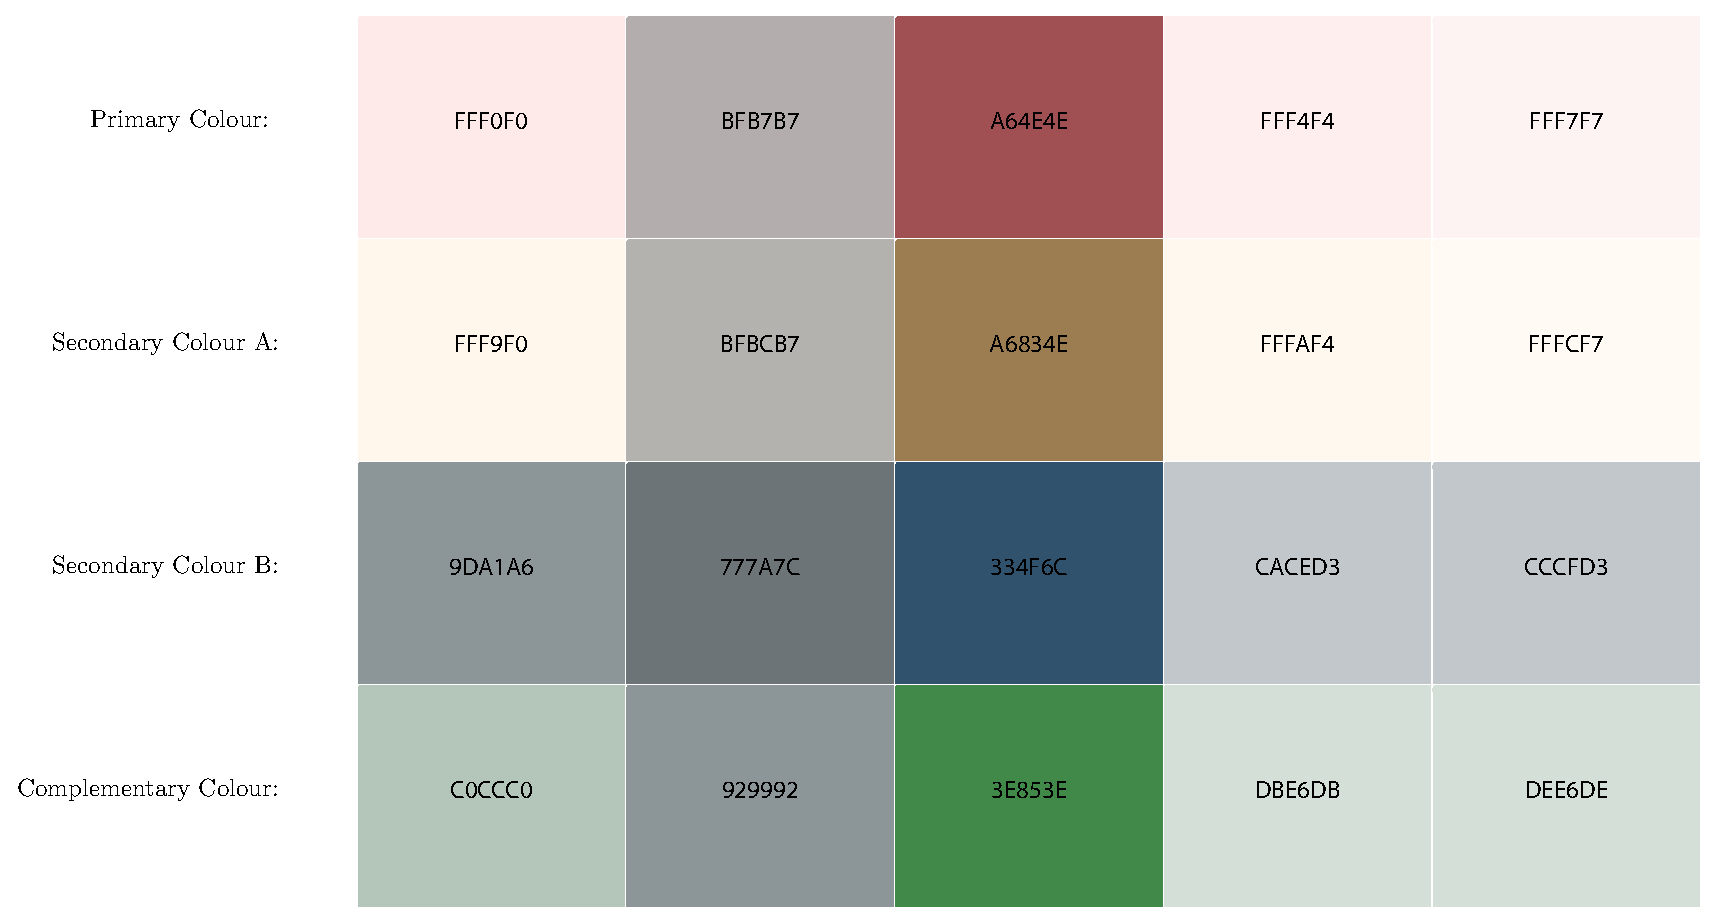
\includegraphics[width=.45\textwidth]{img/colour-scheme.eps}
	\caption{Colour scheme of the interface \protect\cite{colorschemedesigner.com}}
	\label{fig:colour-scheme}
\end{figure}
\todo[inline]{colorschemedesigner.com citep}

\section{Constraints}
The constraints can be divided into groups: layout-/content-based, global/topic/neighbouring, 


Technical argumentation for choices.
Business case argumentation for choices (user needs).
Reference to written articles about design choices -- navigation: sections + headlines, 

\subsection{Layout Constraints}
first focus: layout + one sections

3? columns
images/no image
base layout



\subsection{Content Constraints}
Content similarity relationships:
article vs. neighbouring articles
article vs. containing section/topic
article vs. whole newspaper

breaking
``[...] it was found that the best eight-item  mix within an issue was not necessarily composed of the eight highest-readership items in that issue.'' \cite{EditorsDilemma} (maximum audience coverage, which is no longer an issue due to personalisation)

\begin{align*}
\mathcal{C} &=	\begin{Bmatrix}
					\texttt{all\_different}(a_i),\\
					\texttt{sim}(a_i, a_{i+1}, 0.7, 0.9), \\
					\texttt{sim}(a_i, a_{i-1}, 0.7, 0.9), \\
					\texttt{sim}(a_i, a_j, 0.3, 0.9)
					%artists_i \ne artists_{i-1} \wedge artists_i \ne artists_{i+1},\\
					%album_i \ne album_{i-1} \wedge album_i \ne album_{i+1},\\
					%\texttt{all\_different}(place_i),\\
					tempo_i < tempo_{i+1} + 10 \wedge tempo_i < tempo_{i-1} + 10 \wedge\\
					tempo_i > tempo_{i-1} - 10 \wedge tempo_i > tempo_{i+1} - 10,\\
					%tempo_i < + 5 \cdot length \cdot tempo_j \wedge\\
					%tempo_i > - 5 \cdot length \cdot tempo_j\ \textbf{for}\ i \ne j,\\
					%keys_i = keys_i \vee keys_i = keys_i \pm 1 \vee keys_i = keys_i \pm 12
				\end{Bmatrix}
\end{align*}


\todo[inline]{AIRussel p. 207 preference constraints. can often be encoded as costs on individual variable assignments. Solved either path-based or local.
p. 216 Minimum-remaining-values, p. 217 Least-constraining-value.}

\todo[inline]{Figure of the system design: Model (user model + meta data + constraints), View (layout + inteactions), Control (cp)}

% section design (end)
%!TEX root = thesis.tex
\chapter{Technical Specification} % (fold)
\label{ch:implementation}
This section describes a technical specification of a direct implementation of the design choices made in the previous chapter in terms of client side and server side tasks.

The proposed design presented in the previous chapter has accounted for the presented requirements and user needs, but there are some requirements that will not be implemented due to prioritisation and time limits.

The in chapter~\ref{ch:design} presented application incorporates the user model, but this chapter will only present how to collect the necessary user data and use it in the application -- and not implement it. It will, however, describe which meta data is needed and how to acquire it.

The social aspects of the system is of cause an important part of it and in terms of the business case, social media are easy channels for awareness. \cite{Tidwell} even states her editorial mix pattern as a social media pattern. Nonetheless, these will not be implemented in the presented application as it does not contribute with new knowledge to field. The gathered news articles to used in this project contained both images and videos, but only images will be considered here. It is however easy to implement the support for videos as the same space allocation principles applies.

Also, the personalised summaries have already been very well explored in the paper \cite{fulltext.pdf} and this project will not try to compete with it, so only the first few sentences will constitute the excerpts from articles to be used on the front page.

The categories used to compose sections of is by no means a full list and they have not been verified, but they are some of the most recurring in popular news sites and are used just in order to proof the concept is possible. Thus, their definitions are not comprehensive either.

Finally, only a selection of the full list of the editorial mix constraints, presented in the proposed design, will be implemented. Furthermore, before the user test was done the implementation had already started leading to the implementation of a fairly complex layout constraint to minimise white space. It turned out that some white space was actually a user preference, but the implementation of the constraint will be presented nonetheless, as it shows a good example of what is possible with the system. 
%
%Whitespace between articles should be minimised. This is not an actual user requirement, but it is included as it a fairly complex layout problem to solve and it shows some aspects of what it can do.


\section{Server for Acquiring and Mining Data for Personalisation}
%\subsection{Spacial, temporal and relational personalisation}
The \cite{DCMI} proposes 15 meta data elements for documents, i.e.\ Title, Creator, Subject, Description, Publisher, Contributor, Date, Type, Format, Identifier, Source, Language, Relation, Coverage and Rights. The articles in this project have been acquired using the \cite{Readability} to scrape web pages of articles given by links from RSS-feeds. This way it is possible to get the full article. Under normal circumstances, these would probably be supplied by a content provider, say through an agreement with newspaper companies or social networks. The Readability API provides several meta data elements for the parsed articles; a domain, a title, a article URL, a URL for a lead image, the author, an article excerpt, a word count and a date of publish. This satisfies many of our needs, but there are still some very crucial calculations to be done, i.e.\ the article relevance according to user topics and similarity between articles.

The analysis of article relevance and similarity to other articles will use the same two types analysis, namely a document using the WordNet and entity comparison using Open Calais. These will be presented in the following two sections.

\todo[inline]{Er der argumenteret for at bruge keywords?}

\subsection{WordNet Enriching Articles}
WordNet is a large lexical database of English words and their relationships in the form of different graphs. WordNet is based on \emph{synsets}, which is a set of synonyms which describes different meanings of the same word. WordNet has hyperonymy and hyponymy graph for noun synsets, which is based on the ISA relation between words. A \emph{hypernym} relation is a generalisation, e.g.\ a hypernym for a bed is a piece of furniture; and a \emph{hyponym} relation is a specification, e.g.\ a hyponym for a bed is a bunkbed. For nouns there also exists the meronymy graph, which is a graph describing the part-whole relation; a chair e.g.\ has a back, a seat and legs. Also, parts are inherited by superordinates, e.g.\ if a chair has legs, then an armchair has legs as well. Furthermore, WordNet has a graph describing elaboration, i.e.\ \emph{troponyms}, of verbs synsets, adjectives organised in terms of antonymy and adverbs which can be be described in terms of adjectives. The synsets, the hypernym and hyponym graph and the troponym graph of WordNet are the most interesting, because they describe different meaning of a given word, whereas the others describes relation to other words.
%Noun hyperonymy, hyponymy or ISA relation
%Noun Meronymy, inherited
%Verb synsets, troponyms: dimensions along which verbs can be elaborated
%Adjectives are organized in terms of antonymy
%adverbs are straightforwardly derived from adjectives via morphological affixation

The initial approach involved computing the tf-idf similarity between articles and the topics and articles in between using the Python libraries for this \cite{NLTK}. This approach works on a bow (bag-of-words) with key words and weights representing a single item. The weight is computed by the number of occurrences in the provided text and a cosine distance determines the similarity. However, Python also provides an interface for working with WordNet. This opens the door to a more in-depth analysis of the obtained news articles. \cite{116262780379.pdf} presents an algorithm for enriching articles using WordNet's hypernym graph. A subgraph of WordNets hypernym graph is generated by the top $20\%$ frequent keywords of an article and weighted by:
$$W(d, f) = 2 \cdot \frac{1}{1+e^{-0.125(d^3\frac{f}{TW})}}-0.5$$

Where $d$ stands for the node's depth in the graph (starting from root and moving downwards), $f$ is the frequency of appearance of the node to the multiple graph paths and $TW$ is the total number of words used to generate the hypernym graph. An example of such a hypernym graph is seen in Figure~\ref{fig:hypernym-graph}.
\begin{figure}[h!tp]
	\myfloatalign
	%\makebox[\textwidth][l]{
		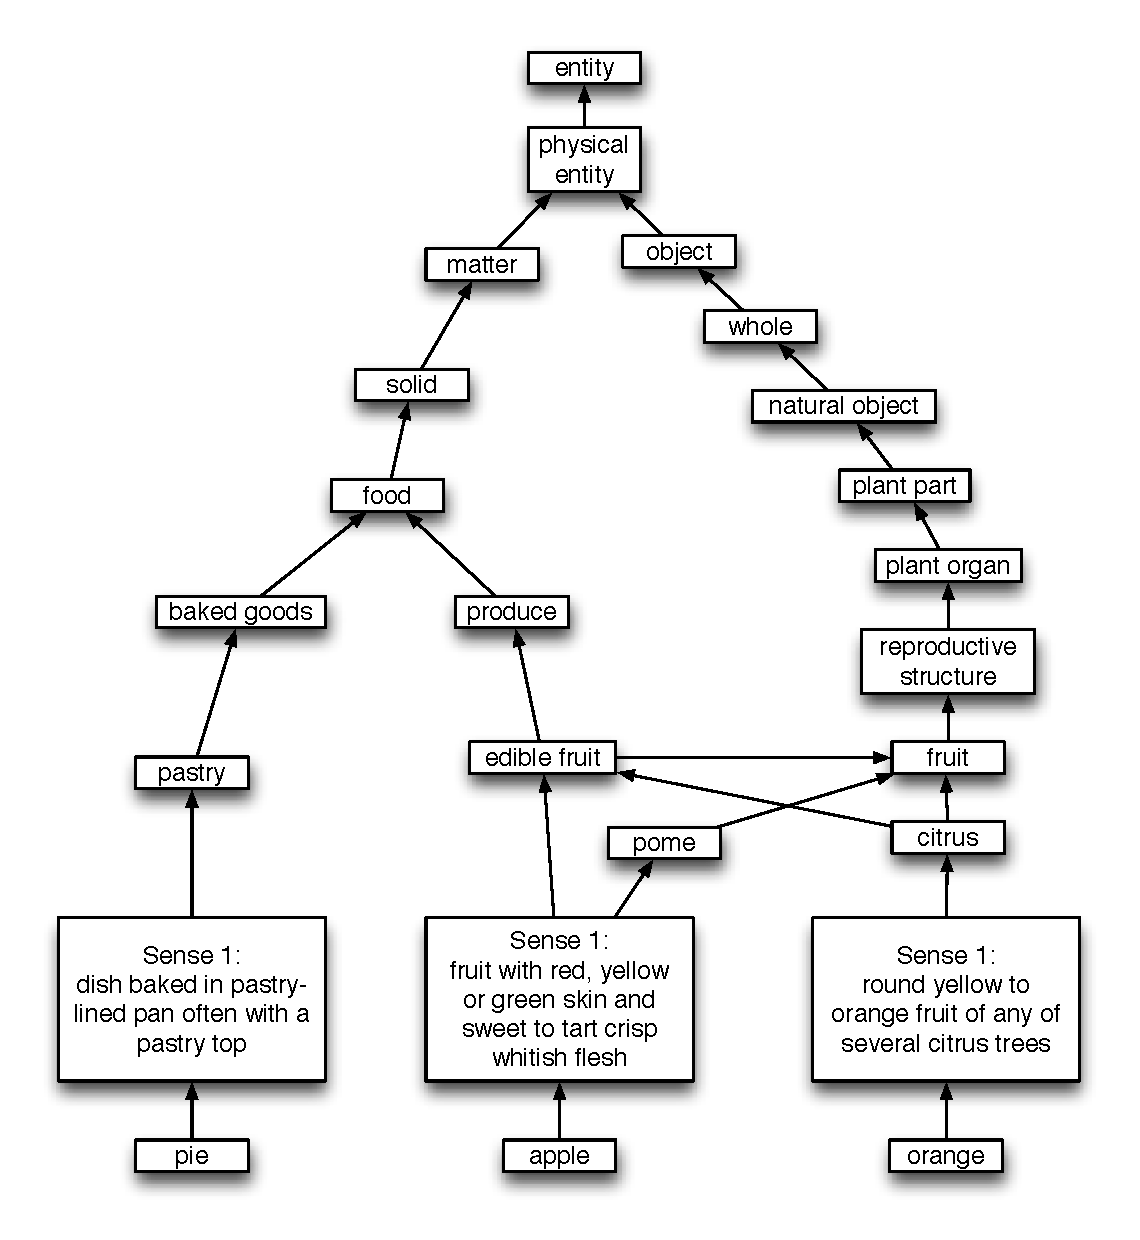
\includegraphics[width=.8\textwidth]{img/hypernym-graph}
	%}
	%\marginnote{
		%\begin{minipage}{\marginparwidth}
			\caption{The figure shows an example of a hypernym graph that could be generated by the \textsc{WordNet Enrich} algorithm.}
			\label{fig:hypernym-graph}
		%\end{minipage}
	%}
\end{figure}


To be able to work with hypernyms, words from articles must be converted to synsets. For each word there exists a synset for each use of the word, with the most frequently used first. Every synset is included at this point, but in a later stage this could be further focused by only using the top $n$. An analysis on how many percent of the words

\todo[inline]{WordNet distinguishes among Types (common nouns) and Instances (specific persons, countries and geographic entities). (\url{http://wordnet.princeton.edu/})}

\todo[inline]{level is only a part Python implementation of WordNet}

\subsection{Meta Data from Open Calais}

\subsection{Computing Similarity}
    - Storing Data

\section{Client for Composing the Editorial Mix and Presenting the Articles}
- Dynamic Page (created from form)
\todo[inline]{css: conditional styling}

\todo[inline]{From the description of the editorial mix it is possible to model

General requirements:

}

\subsection{Interface}

In Figure~\ref{fig:sequence} is shown a sequence diagram of what the system does in order to display the front page (or a section), when the user opens the application.
%\sidecaptionfigure{\textwidth}{img/sequence}{The figure shows a sequence diagram from when the user chooses a topic category until he can read articles from this topic. \texttt{secNum} is the section number to display (the front page is section 0), \texttt{userId} is a string that identifies the user, \texttt{userPrefs} is the user preferences on the specific section and \texttt{articles} is the library of articles to compose the editorial mix of.}{fig:sequence}
%\begin{figure}[h!tp]
%	\myfloatalign
%	\makebox[\textwidth][l]{
%		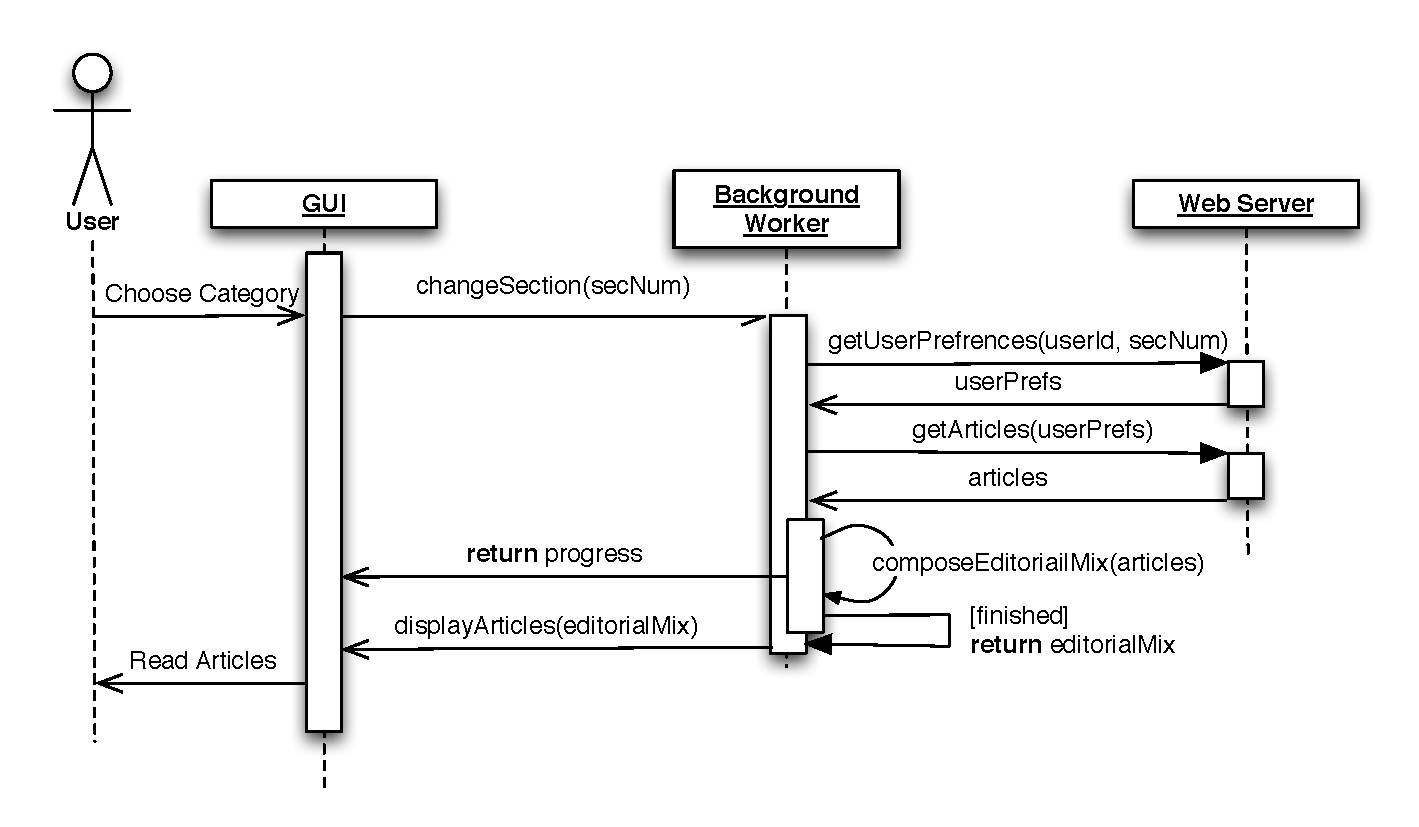
\includegraphics[width=.8\largefigure]{img/sequence}
%	}
%	\marginnote{
%	\vspace{-50pt}
%	\begin{minipage}{\marginparwidth}
%		\caption{A sequence diagram from when the user chooses a topic category until reading articles. \texttt{secNum} is a section number, (front page is section $0$), \texttt{userId} the user id, \texttt{%userPrefs} the user preferences on a given section and \texttt{articles} is a library of articles to compose the editorial mix of.}
%	\label{fig:sequence}
%		\end{minipage}
%	}
%\end{figure}
\begin{figure}[h!tp]
	\centering
	
	\def\mygraphic{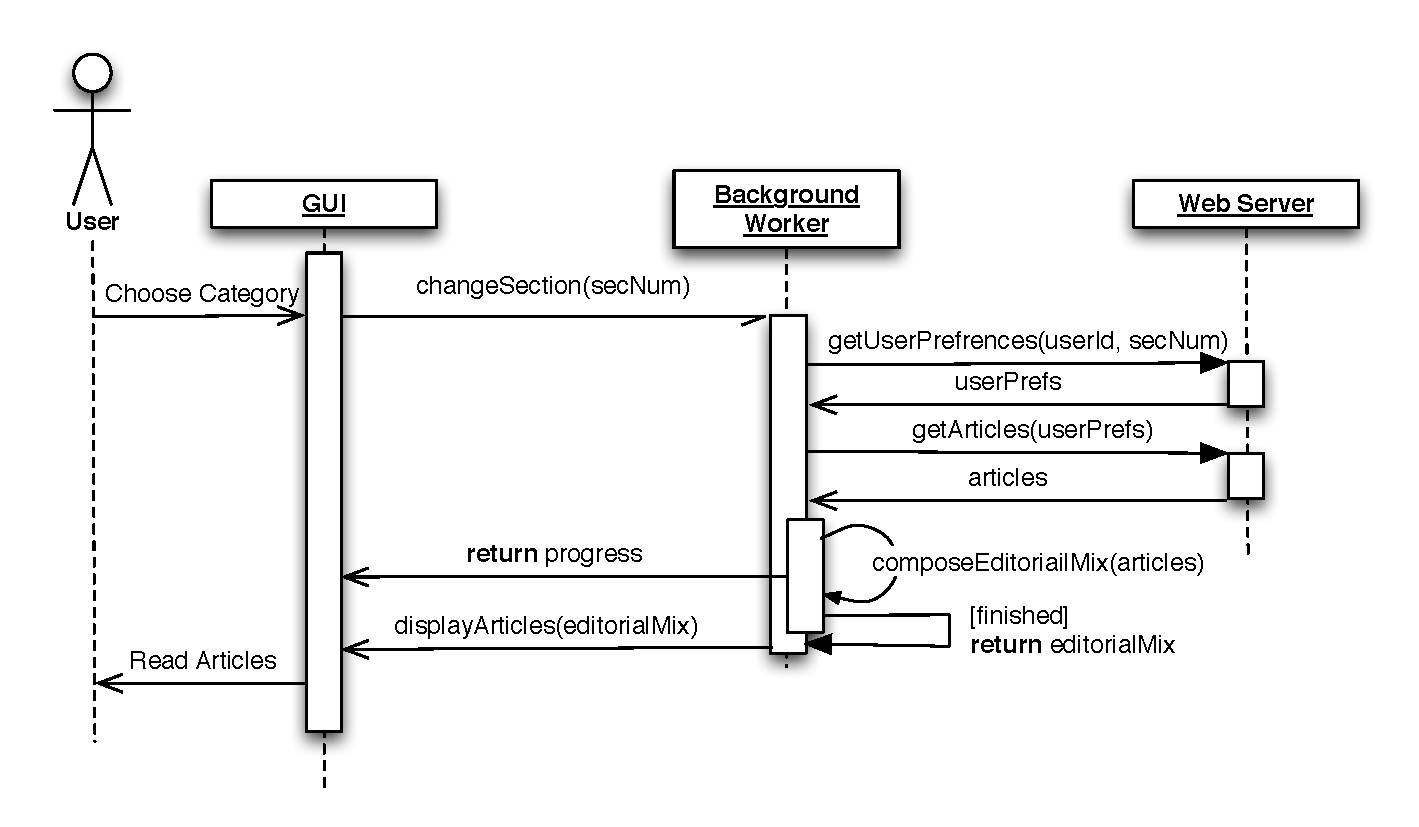
\includegraphics[width=\textwidth]{img/sequence}}
	%\newlength{\graphicheight}
	\settoheight\graphicheight{\mygraphic}
	\mygraphic
	\marginnote{
	\begin{minipage}{\marginparwidth}
		\vspace{-\graphicheight}%
		\caption{A sequence diagram from when the user chooses a topic category until reading articles. \texttt{secNum} is a section number, (front page is section $0$), \texttt{userId} the user id, \texttt{userPrefs} the user preferences on a given section and \texttt{articles} is a library of articles to compose the editorial mix of.}
		\label{fig:sequence}
		\vspace{\graphicheight}
		\end{minipage}
	}
\end{figure}
%\begin{figure}[h!tp]
%	\myfloatalign
%		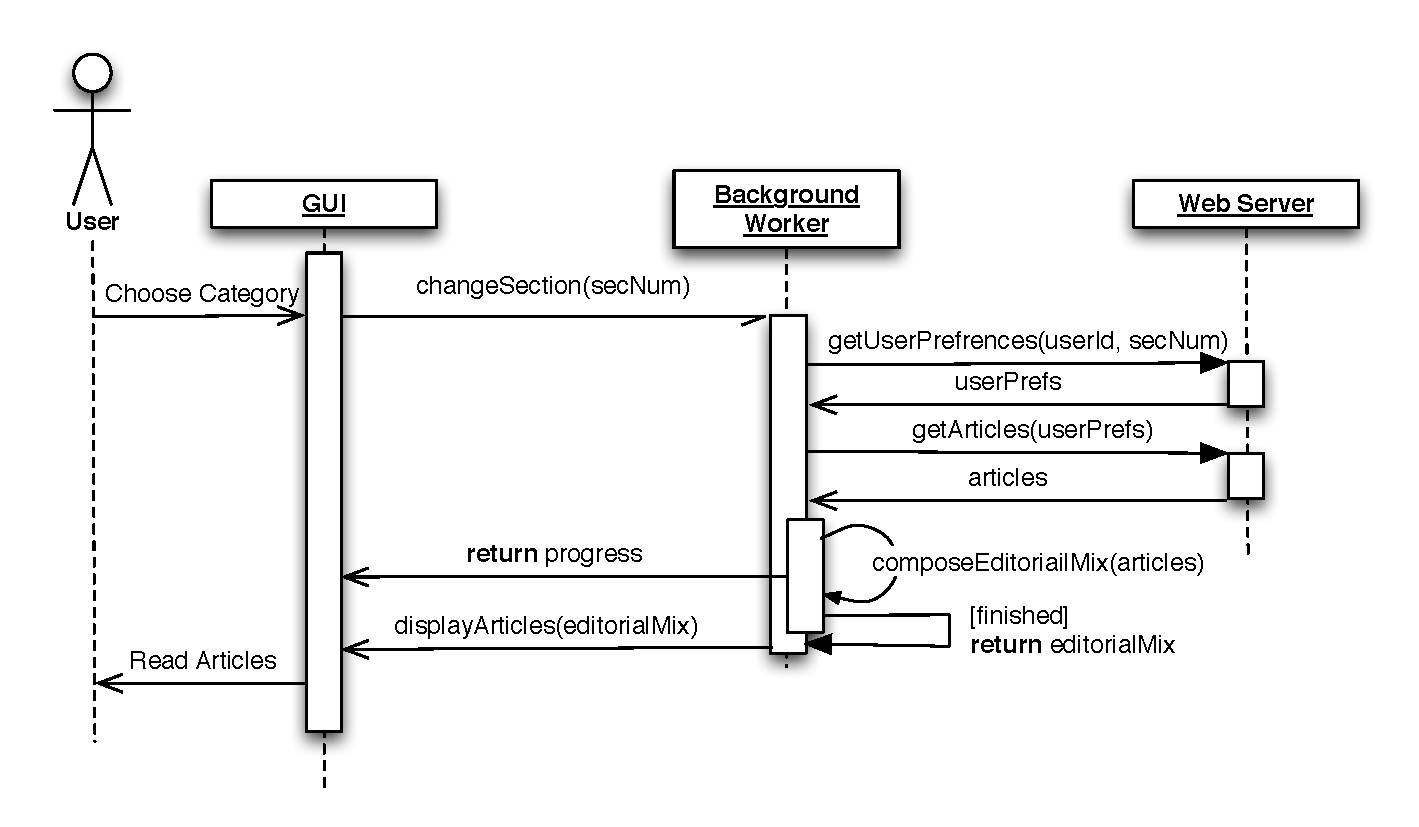
\includegraphics[width=\textwidth]{img/sequence}
%	\caption{The figure shows a sequence diagram from when the user chooses a topic category until he can read articles from this topic. \texttt{secNum} is the section number to display (the front page is section 0), \texttt{userId} is a string that identifies the user, \texttt{userPrefs} is the user preferences on the specific section and \texttt{articles} is the library of articles to compose the editorial mix of.}
%	\label{fig:sequence}
%\end{figure}

When the application is opened, or the application is changed to display a section, a background worker is initialised to compose its containing mix of articles. Of cause, if the mix of articles in a section, or the front page, have already been computed, it should not have to recompute it. The background worker needs to get both the user preferences of the chosen topic category and articles that potentially fit the user preferences. While the worker computes the editorial mix it sends messages to the user interface about the progress, to provide feedback to the user. When it finishes the user interface is asked to display the articles.



\subsection{Constraint Personalisation Library}

\subsubsection{Data Structure}
\subsubsection{General Purpose Solver}

\subsection{Backend worker.js}
  - Lazy Loading Sections
  - Knowledge Passing

worker i tråd for sig selv, men samme proces

worker.js to create a background worker to perform the constriant programming.

Model-View-Control using backbone.js

Paging: single page web apps + manipulation the browser history \url{https://developer.mozilla.org/en/DOM/Manipulating_the_browser_history}

Preference ordering of hard constraints or division between preference constraints and hard constraints.

Assignment from library in stead of arbitrary assignment? The latter is a more hypothetical approach. Providing the library as a constraint, where each variable assignment must have a unique combination from one of the possibilities of the constraint.
(sim,breaking,chars,date,sections?,columns):list
The former introduces an implicit constraint in that the general purpose solver can only choose from the library, thus can only choose a combination of values that exists.

Ranges can be optimised in space by converting them to integer ranges. This can be done by setting min = 0 and max = (b-a)/gap.

Furthermore each subdomain should be able to be represented by a set of ranges and atomic values. Propagating through values causes many iterations and a whole range may be discarded by looking at its maximum and minimum value. However, if the range holds a potential valid value (solution to a variable) it can be divided into smaller ranges and their minimum and maximum values may be examined. This divide-and-conquer technique may continue until the search reaches atomic values (determined by the gap value of the range). If some atomic values and ranges seems to fulfil the constraints they should be returned. And the subdomain now consists of both ranges and atomic values.

Optimal/promising
fixed budget computation

The library could take any combination of constraints and then organise them into conjunctions of disjunctions, with the constraints taking fewer values first.

In the implementation this is done by hand, so the program takes conjunctions of disjunctions of constraints organised with constraints that takes fewer values first. Constraint weighing could also help organising the disjunctions and furthermore lead the search to concentrate on variables that is bound by these constraints. (p. 222 AIRussel).

Constraints should point to specific variables, this makes it somewhat rigid/ineffective because I have to write at global constraint that accounts for everything (ineffective in propagation -- might also be a problem if it does not show progress in changing values, i.e.\ it is a hard constraints and not returning a cost of the set of values.) or divide it into smaller constraints separated by an `or' (v). The latter is ineffective because there would should be a combination of constraints accounting for every situation, e.g. if the first variable is satisfying an unary constraint, the next say 3 variables (if the problem holds 4 variables) could satisfy three unary constraints, an unary and a binary (two combinations exists) or a constraint that takes three variables. This grows fast with the number of constraints.

\todo[inline]{Does it make sense that a continuous range cannot have specific values removed? Should it be possible for it be divided into subranges if the user decides to remove a range of values in between its domain of [min;max]?}

Pool of workers to compute sections and send results to another worker to handle front page articles. Or, a lazy load approach where the front page is computed and then sections are computed with hard constraints that manages placement of articles within the given sections, e.g.\ if an article from the front page has the potential to be placed in only one section the constraint should state this, but it would demand cross-worker-constraints to handle if an article from the front page has the potential to be placed in more section (i.e.\ \texttt{xor}). color

Reducing constraints to binary constraints.

\todo[inline]{Implement visual difference between featured articles and non-featured articles.}

% section design (end)
%!TEX root = thesis.tex
\chapter{Evaluation of the Solution} % (fold)
\label{ch:evaluation}

Evaluate using the in \cite{Sections-categories-and-keywords-as-interest-specification-tools-for-personalised-news-services.pdf} and \cite{Evaluating-a-User-Model-Based-Personalisation-Architecture-for-Digital-News-Services.pdf} presented method. Their categorisation based on few keywords (5 as the lowest) to represent a category resulted in poor evaluation, this gives a good motivation for including more keywords and using Wordnet to enrich the set of keywords.

It could be interesting to evaluate the precision and recall points based on: news items per section, news items per category, maximum number of news items per message required by the user, general relevance of the contents of a given day for a given user, etc. as \cite{Sections,-categories-and-keywords-as-interest-specification-tools-for-personalised-news-services.pdf} proposes.

\cite{Sections,-categories-and-keywords-as-interest-specification-tools-for-personalised-news-services.pdf} also raise the problem of precision in finding news within based on a single day. This can hopefully be handled by having the user specify in which period of time he wants news and maybe notify the user that solutions might be inaccurate if a limited period of time is chosen, or just limit the user to specify 24 hours as a minimal value.
%``just as newspaper must come full of news everyday, regardless of whether anything interesting has happened or not, newspaper sections will carry a certain amount of news independently of their relevance to the section heading, and a personalised news message will feature some news item distantly related to the user profile.''


\subsection{Initial Test}
\todo[inline]{NOT ONLY 5 test persons \protect\cite{NielsenTest}. This has been discarded by many.}
%\cite{NielsenTest} says that 5 test persons in a qualitative test is enough to uncover most preferences and issues, but the test included 7 test persons to be more adequate.

\subsection{Result}

\section{Test}

\subsection{Layout}

columns constraints, white space and odd placement of articles.

In order to come closer to understanding what newspapers does it could be interesting to analyse their component structure, e.g.\ using \cite{00953970.pdf} algorithm.


\subsection{Content}
The system can be used for automatic classification of articles. Of cause, then a sufficient list of categories and their definitions must be used. This can either be retrieved by the list of Google News categories\footnote{\url{http://support.google.com/webmasters/bin/answer.py?hl=en&answer=42993}.} and a Wordnet enriched list of key words from Google News list of suggested keywords\footnote{\url{http://support.google.com/news/publisher/bin/answer.py?hl=en&answer=116037}.} or by the root terms presented in \cite{10-1-1-19-5583}. These can later on be refined by information retrieved by the user behaviour in the system and manually removal of false negatives? However, also more advanced techniques of text classification could be used in later stages of the system, like one presented in \cite{Evaluating-a-User-Model-Based-Personalisation-Architecture-for-Digital-News-Services.pdf}.

\todo[inline]{Maybe find a better example of text classification.}

Use of automatic generation of personal item summaries \cite{fulltext.pdf}


Use geotargeting to supply local news.

Use a thesaurus and predefined root terms as in \cite{10-1-1-19-5583} which improves classification; semantic knowledge is more general than keywords.

\subsection{Functionality}
Order a print copy of the newspaper



The development of the Internet from a distributor of information to a library of digital applications has deeply integrated the users in every step of an applications lifetime. It has become harder to distinguish between super users and developers, applications are branched and modified according to every need and authors can therefore no longer predict which use his application can be to another user -- nor should he have to.

\subsection{Improvements}
\cite{Personalizing-your-electronic-newspaper.pdf} suggest virtual communities, or individuals with common interests.

Weights on key words should be adjusted by a strength (or an uncertainty) of prediction as it is proposed in \cite{10.1.1.45.5230.pdf}.

Count the number of sources have included an articles that are very similar to find the breaking factor.

How to handle that a user is not presented with an already read article? \cite{User-Modeling-for-Adaptive-News-Access.pdf} presents the nearest neighbour (NN) algorithm approach, using a tf-idf similarity, to determine whether the story is already known, i.e.\ the similarity to the NN read story is above a given threshold. This could be solved by keeping a library of read items (this can be done along with the tracking of which article is in focus) and then match new items against this banned list and down prioritise them if their similarity is too high. This could be done with the same polynomial function as used between articles.

``Distinguishing between short-term and long-term models has several desirable qualities in domains with temporal characteristics (Chiu and Webb, 1998).'' \cite{User-Modeling-for-Adaptive-News-Access.pdf}.

% section evaluation (end)
%!TEX root = thesis.tex
\chapter{Conclusion} % (fold)
\label{ch:conclusion}

% section conclusion (end)

%% Chapter 2

\chapter{Examples} % Chapter title

\label{ch:examples} % For referencing the chapter elsewhere, use \autoref{ch:examples} 

%----------------------------------------------------------------------------------------

\lipsum[1]

%----------------------------------------------------------------------------------------

\section{A New Section}

\lipsum[2]

Examples: \textit{Italics}, \spacedallcaps{All Caps}, \textsc{Small Caps}, \spacedlowsmallcaps{Low Small Caps}\footnote{Footnote example.}.

%------------------------------------------------

\subsection{Test for a Subsection}

\graffito{Note: The content of this chapter is just some dummy text.}
\lipsum[3-5]

%------------------------------------------------

\subsection{Autem Timeam}

\lipsum[6]

%----------------------------------------------------------------------------------------

\section{Another Section in This Chapter}

\lipsum[7]

Sia ma sine svedese americas. Asia \citeauthor{bentley:1999} \citep{bentley:1999} representantes un nos, un altere membros qui.\footnote{De web nostre historia angloromanic.} Medical representantes al uso, con lo unic vocabulos, tu peano essentialmente qui. Lo malo laborava anteriormente uso.

\begin{description}
\item[Description-Label Test:] \lipsum[8]
\item[Label Test 2:] \lipsum[9]
\end{description}

\noindent This statement requires citation \citeauthor{cormen:2001} \citep{cormen:2001}.

%------------------------------------------------

\subsection{Personas Initialmente}

\lipsum[10]

\subsubsection{A Subsubsection}
\lipsum[11]

\paragraph{A Paragraph Example} \lipsum[12]

\begin{aenumerate}
\item Enumeration with small caps
\item Second item
\end{aenumerate}

\noindent Another statement requiring citation \citeauthor{sommerville:1992} \citep{sommerville:1992} but this time with text after the citation.

\begin{table}
\myfloatalign
\begin{tabularx}{\textwidth}{Xll} \toprule
\tableheadline{labitur bonorum pri no} & \tableheadline{que vista}
& \tableheadline{human} \\ \midrule
fastidii ea ius & germano &  demonstratea \\
suscipit instructior & titulo & personas \\
\midrule
quaestio philosophia & facto & demonstrated \citeauthor{knuth:1976} \\
\bottomrule
\end{tabularx}
\caption[Autem timeam deleniti usu id]{Autem timeam deleniti usu id. \citeauthor{knuth:1976}}  
\label{tab:example}
\end{table}

\enlargethispage{2cm}

%------------------------------------------------

\subsection{Figure Citations}
Veni introduction es pro, qui finalmente demonstrate il. E tamben anglese programma uno. Sed le debitas demonstrate. Non russo existe o, facite linguistic registrate se nos. Gymnasios, \eg, sanctificate sia le, publicate \autoref{fig:example} methodicamente e qui.

Lo sed apprende instruite. Que altere responder su, pan ma, \ie, signo studio. \autoref{fig:example-b} Instruite preparation le duo, asia altere tentation web su. Via unic facto rapide de, iste questiones methodicamente o uno, nos al.

\begin{figure}[bth]
\myfloatalign
\subfloat[Asia personas duo.]
{\includegraphics[width=.45\linewidth]{img/example_1}} \quad
\subfloat[Pan ma signo.]
{\label{fig:example-b}
\includegraphics[width=.45\linewidth]{img/example_2}} \\
\subfloat[Methodicamente o uno.]
{\includegraphics[width=.45\linewidth]{img/example_3}} \quad
\subfloat[Titulo debitas.]
{\includegraphics[width=.45\linewidth]{img/example_4}}
\caption[Tu duo titulo debitas latente]{Tu duo titulo debitas latente.}\label{fig:example}
\end{figure} % Chapter 2
%% Chapter 3

\chapter{Math Test Chapter} % Chapter title

\label{ch:mathtest} % For referencing the chapter elsewhere, use \autoref{ch:mathtest}

%----------------------------------------------------------------------------------------

\lipsum[13]

%----------------------------------------------------------------------------------------

\section{Some Formulas}

Due to the statistical nature of ionisation energy loss, large fluctuations can occur in the amount of energy deposited by a particle traversing an absorber element\footnote{Examples taken from Walter Schmidt's great gallery: \\ \url{http://home.vrweb.de/~was/mathfonts.html}}.  Continuous processes such as multiple scattering and energy loss play a relevant role in the longitudinal and lateral development of electromagnetic and hadronic showers, and in the case of sampling calorimeters the measured resolution can be significantly affected by such fluctuations in their active layers.  The description of ionisation fluctuations is characterised by the significance parameter $\kappa$, which is proportional to the ratio of mean energy loss to the maximum allowed energy transfer in a single collision with an atomic electron: \graffito{You might get unexpected results using math in chapter or section heads. Consider the \texttt{pdfspacing} option.}
\begin{equation}
\kappa =\frac{\xi}{E_{\mathrm{max}}} %\mathbb{ZNR}
\end{equation}
$E_{\mathrm{max}}$ is the maximum transferable energy in a single collision with an atomic electron.
\[E_{\mathrm{max}} =\frac{2 m_{\mathrm{e}} \beta^2\gamma^2 }{1 + 2\gamma m_{\mathrm{e}}/m_{\mathrm{x}} + \left ( m_{\mathrm{e}} /m_{\mathrm{x}}\right)^2}\ ,\]
where $\gamma = E/m_{\mathrm{x}}$, $E$ is energy and $m_{\mathrm{x}}$ the mass of the incident particle, $\beta^2 = 1 - 1/\gamma^2$ and $m_{\mathrm{e}}$ is the electron mass. $\xi$ comes from the Rutherford scattering cross section and is defined as:
\begin{eqnarray*} \xi  = \frac{2\pi z^2 e^4 N_{\mathrm{Av}} Z \rho
\delta x}{m_{\mathrm{e}} \beta^2 c^2 A} =  153.4 \frac{z^2}{\beta^2}
\frac{Z}{A}
\rho \delta x \quad\mathrm{keV},
\end{eqnarray*}
where

\begin{tabular}{ll}
$z$ & charge of the incident particle \\
$N_{\mathrm{Av}}$ & Avogadro's number \\
$Z$ & atomic number of the material \\
$A$ & atomic weight of the material \\
$\rho$ & density \\
$ \delta x$ & thickness of the material \\
\end{tabular}

$\kappa$ measures the contribution of the collisions with energy transfer close to $E_{\mathrm{max}}$.  For a given absorber, $\kappa$ tends towards large values if $\delta x$ is large and/or if $\beta$ is small.  Likewise, $\kappa$ tends towards zero if $\delta x $ is small and/or if $\beta$ approaches $1$.

The value of $\kappa$ distinguishes two regimes which occur in the description of ionisation fluctuations:

\begin{enumerate}
\item A large number of collisions involving the loss of all or most of the incident particle energy during the traversal of an absorber.

As the total energy transfer is composed of a multitude of small energy losses, we can apply the central limit theorem and describe the fluctuations by a Gaussian distribution. This case is applicable to non-relativistic particles and is described by the inequality $\kappa > 10 $ (\ie, when the mean energy loss in the absorber is greater than the maximum energy transfer in a single collision).

\item Particles traversing thin counters and incident electrons under any conditions.

The relevant inequalities and distributions are $ 0.01 < \kappa < 10 $, Vavilov distribution, and $\kappa < 0.01 $, Landau distribution.
\end{enumerate}

%----------------------------------------------------------------------------------------

\section{Various Mathematical Examples}

If $n > 2$, the identity \[t[u_1,\dots,u_n] = t\bigl[t[u_1,\dots,u_{n_1}], t[u_2,\dots,u_n] \bigr]\] defines $t[u_1,\dots,u_n]$ recursively, and it can be shown that the alternative definition \[t[u_1,\dots,u_n] = t\bigl[t[u_1,u_2],\dots,t[u_{n-1},u_n]\bigr]\] gives the same result. % Chapter 3
%% Chapter X

\chapter{Chapter Title} % Chapter title

\label{ch:name} % For referencing the chapter elsewhere, use \autoref{ch:name} 

%----------------------------------------------------------------------------------------

\section{Section Title}

Content

%------------------------------------------------

\subsection{Subsection Title}

Content

%------------------------------------------------

\subsection{Subsection Title}

Content

%----------------------------------------------------------------------------------------

\section{Section Title}

Content % Chapter 4 - empty template


%----------------------------------------------------------------------------------------
%	THESIS CONTENT - APPENDICES
%----------------------------------------------------------------------------------------

\appendix

\part{Appendix} % New part of the thesis for the appendix

%!TEX root = ../thesis.tex
\chapter{User Needs}
\label{appendix:user-needs}
This section will define the user needs for the application.

\section{Personas}
%http://www.pewinternet.org/Reports/2010/Generations-2010.aspx 2010
%http://epp.eurostat.ec.europa.eu/portal/page/portal/statistics/search_database
%http://epp.eurostat.ec.europa.eu/tgm/table.do?tab=table&init=1&plugin=1&language=en&pcode=tin00097
%Individuals using the Internet for reading / downloading online newspapers / news magazines (tin00097)
\begin{figure}[h!tp]
\myfloatalign
\subfloat[Initial prototype layout with adjustable ratios between articles and a paged interface of each section.]{
  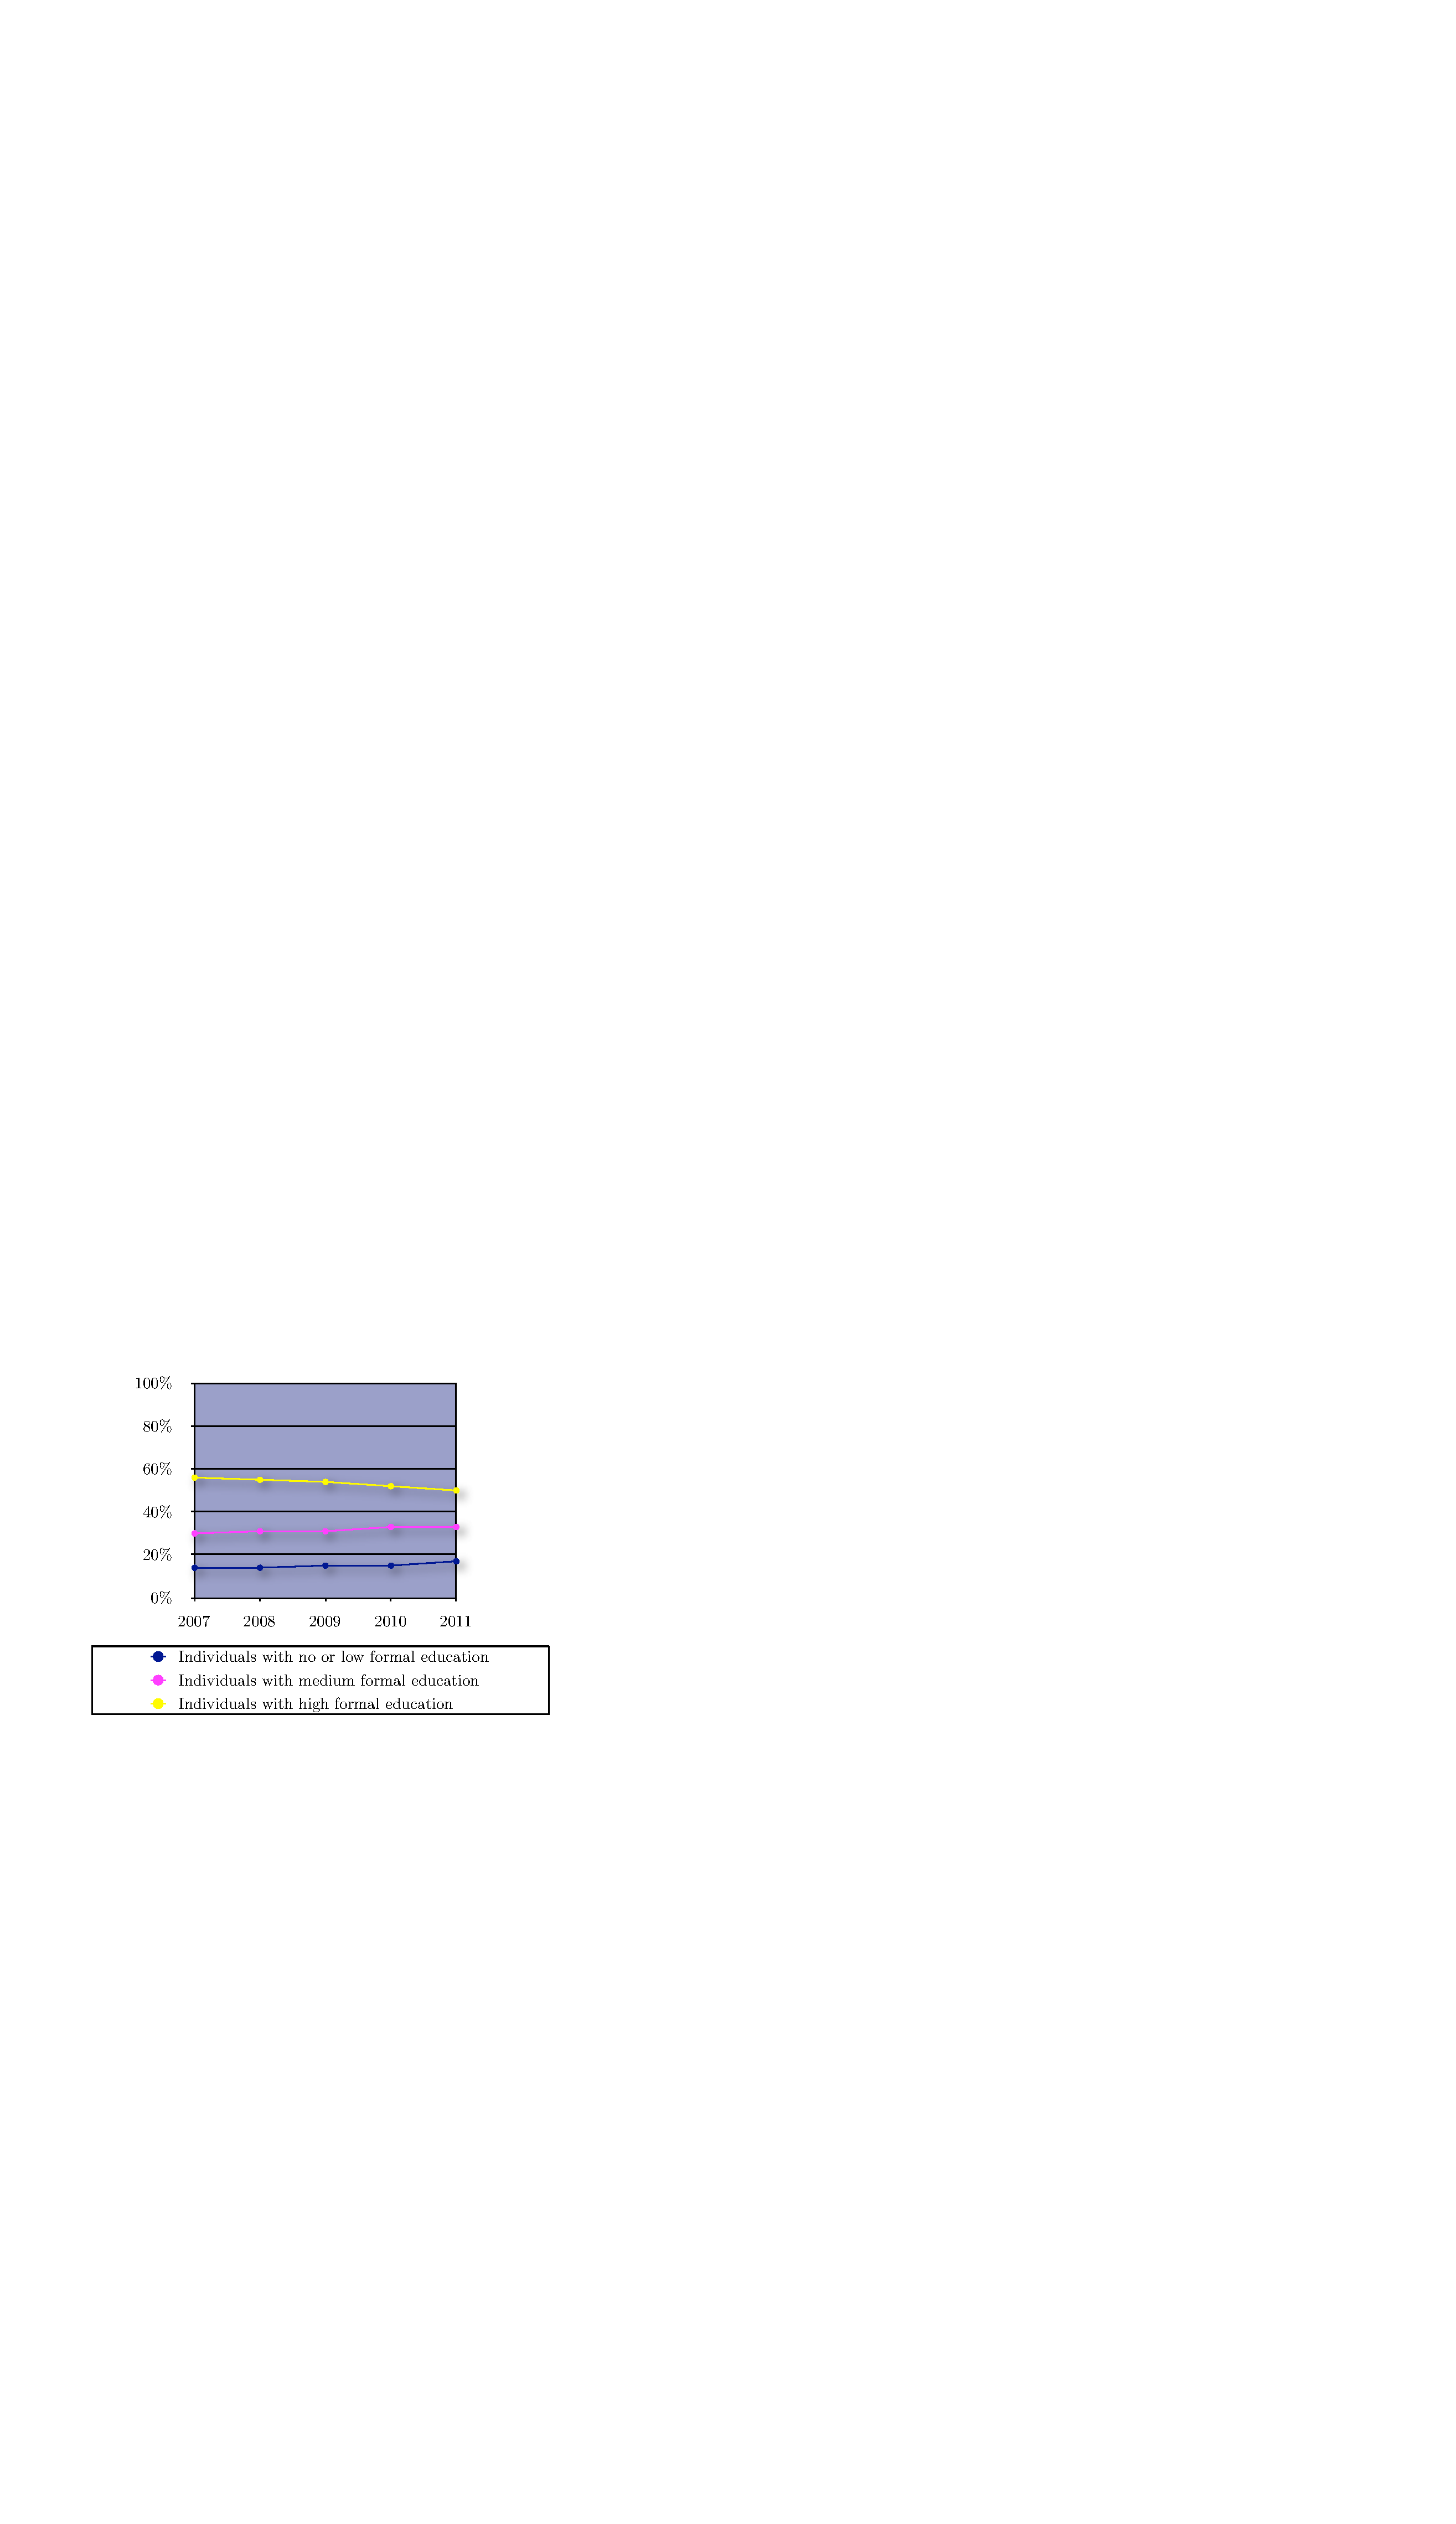
\includegraphics[width=.4\textwidth]{img/chart-educational.pdf}
  %\label{fig:prototype-iteration1}
} \qquad
\subfloat[Second iteration of the prototype with an ``endless'' layout. Sections are placed beneath each other.]{
  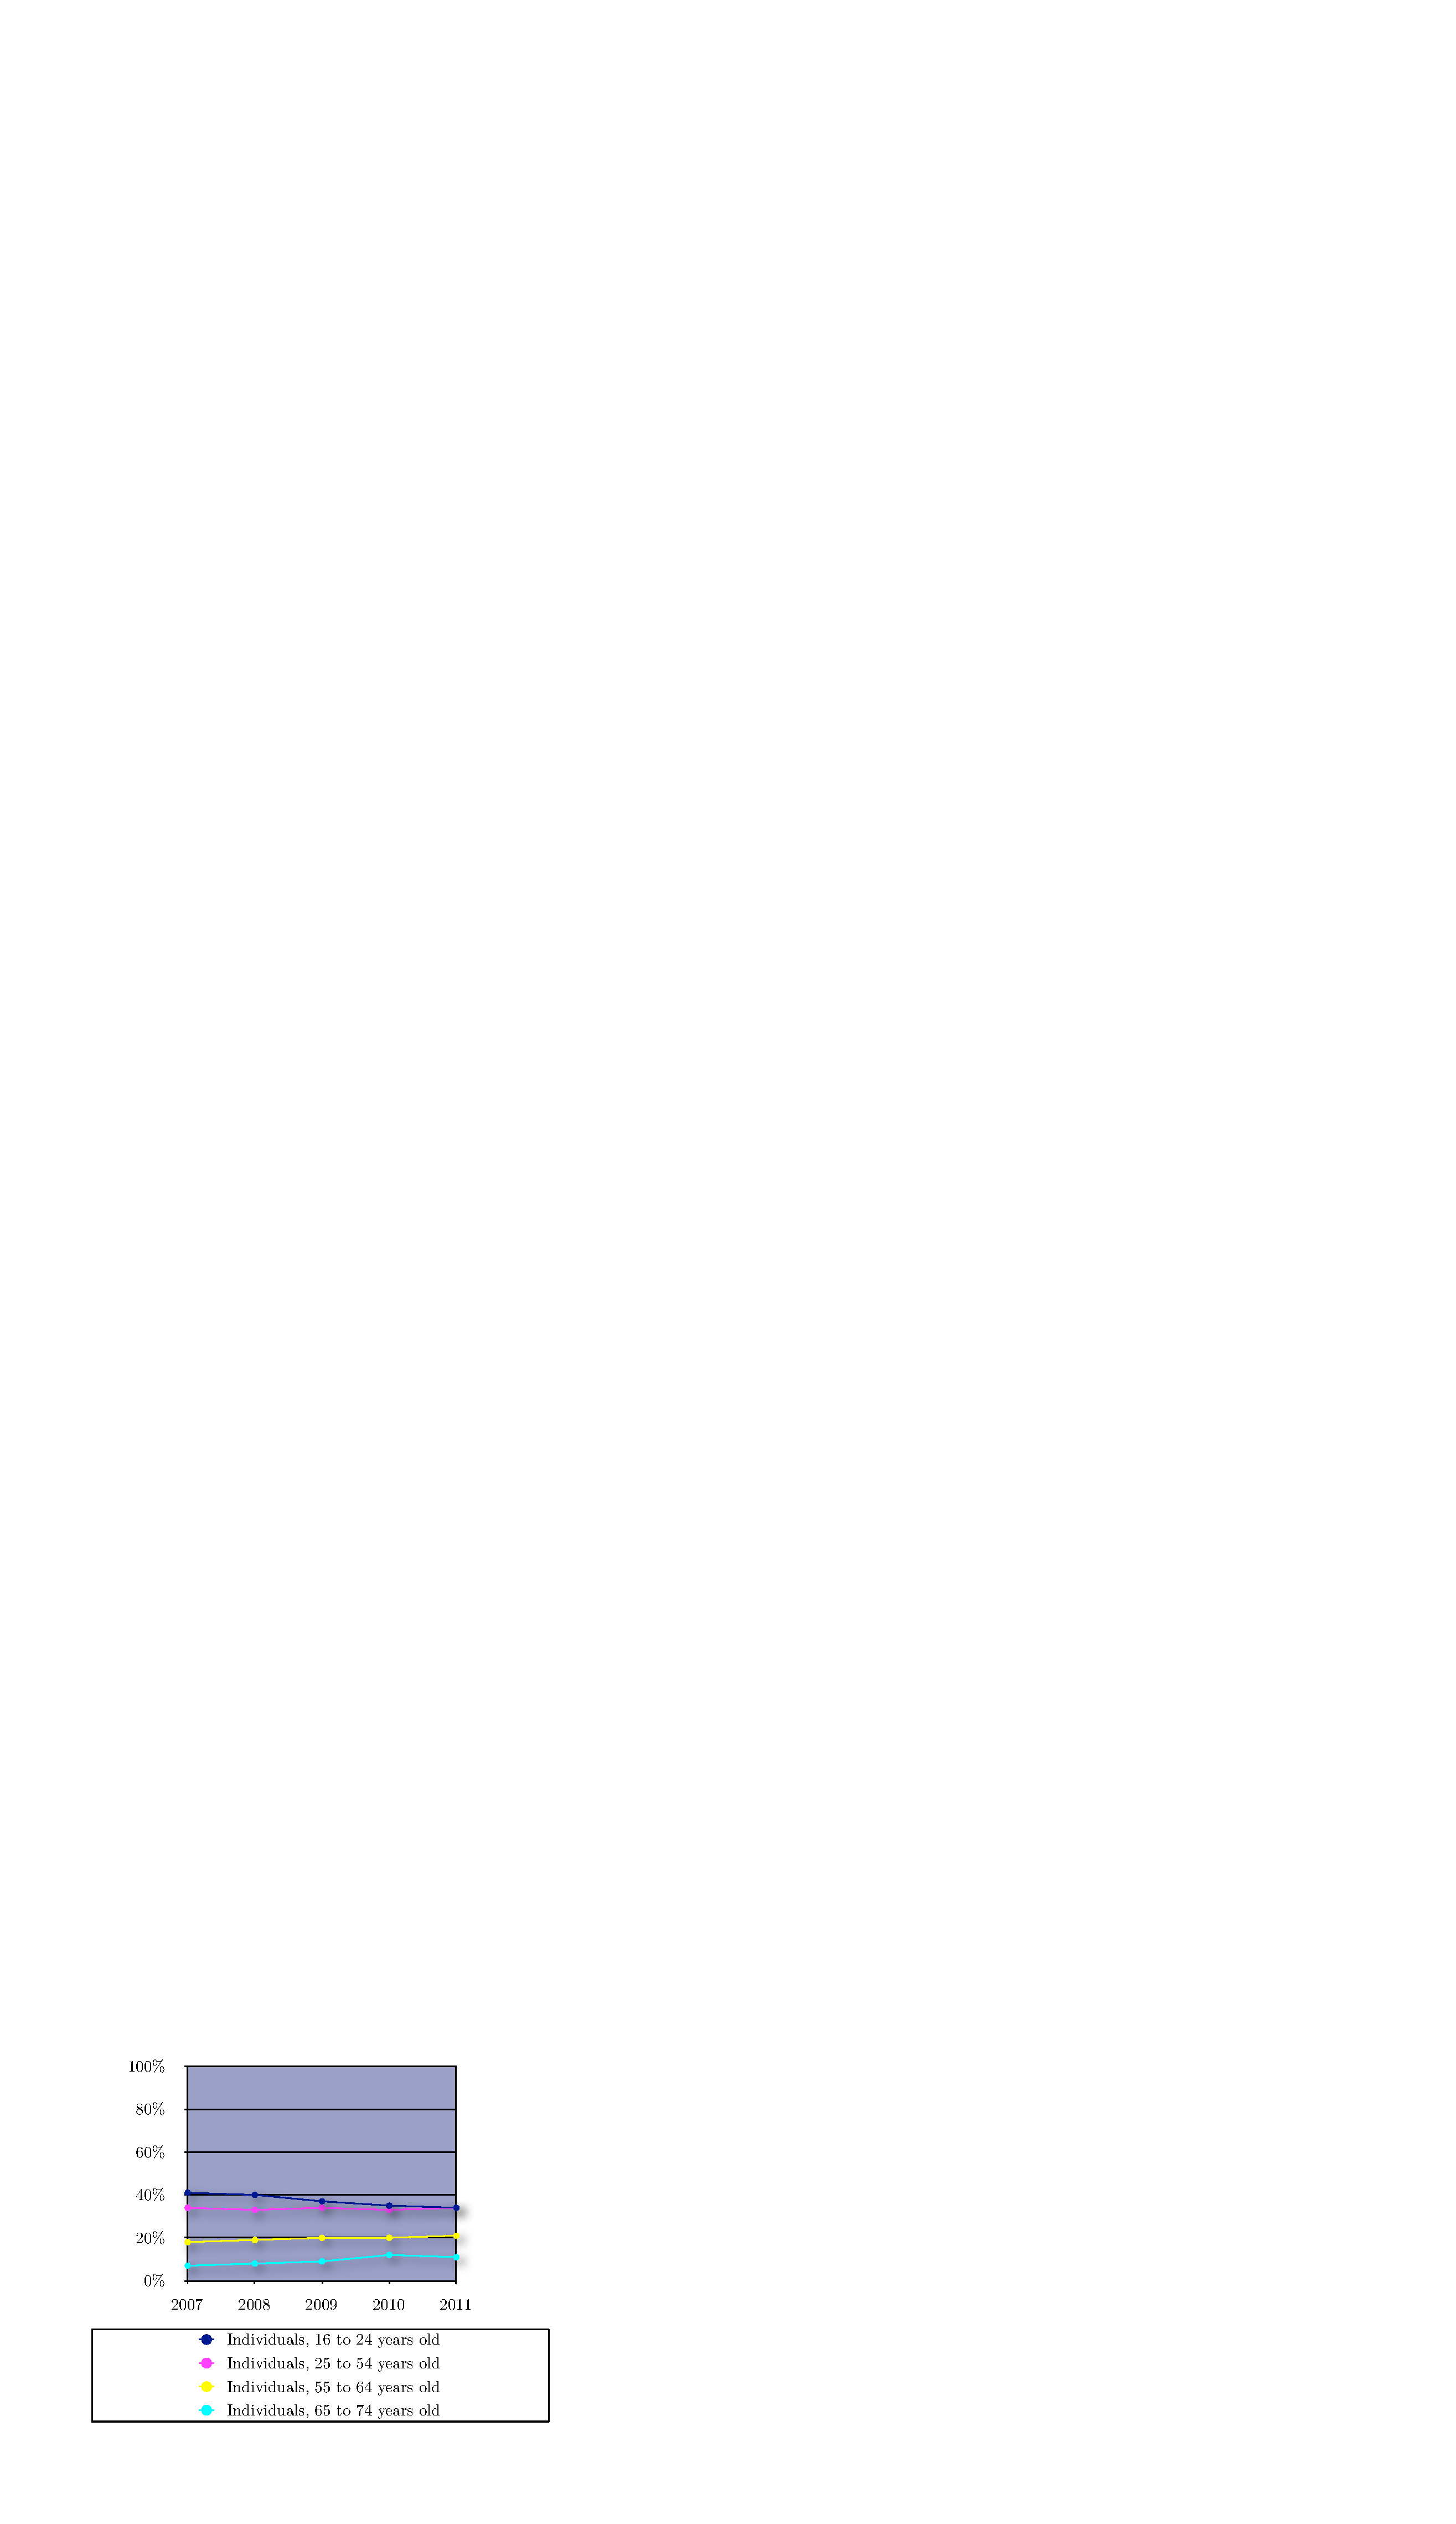
\includegraphics[width=.4\textwidth]{img/chart-individuals.pdf}
  %\label{fig:prototype-iteration2}
} \\
\subfloat[Third iteration of the prototype with a column-based and ``endless'' layout. Sections are placed beneath each other.]{
  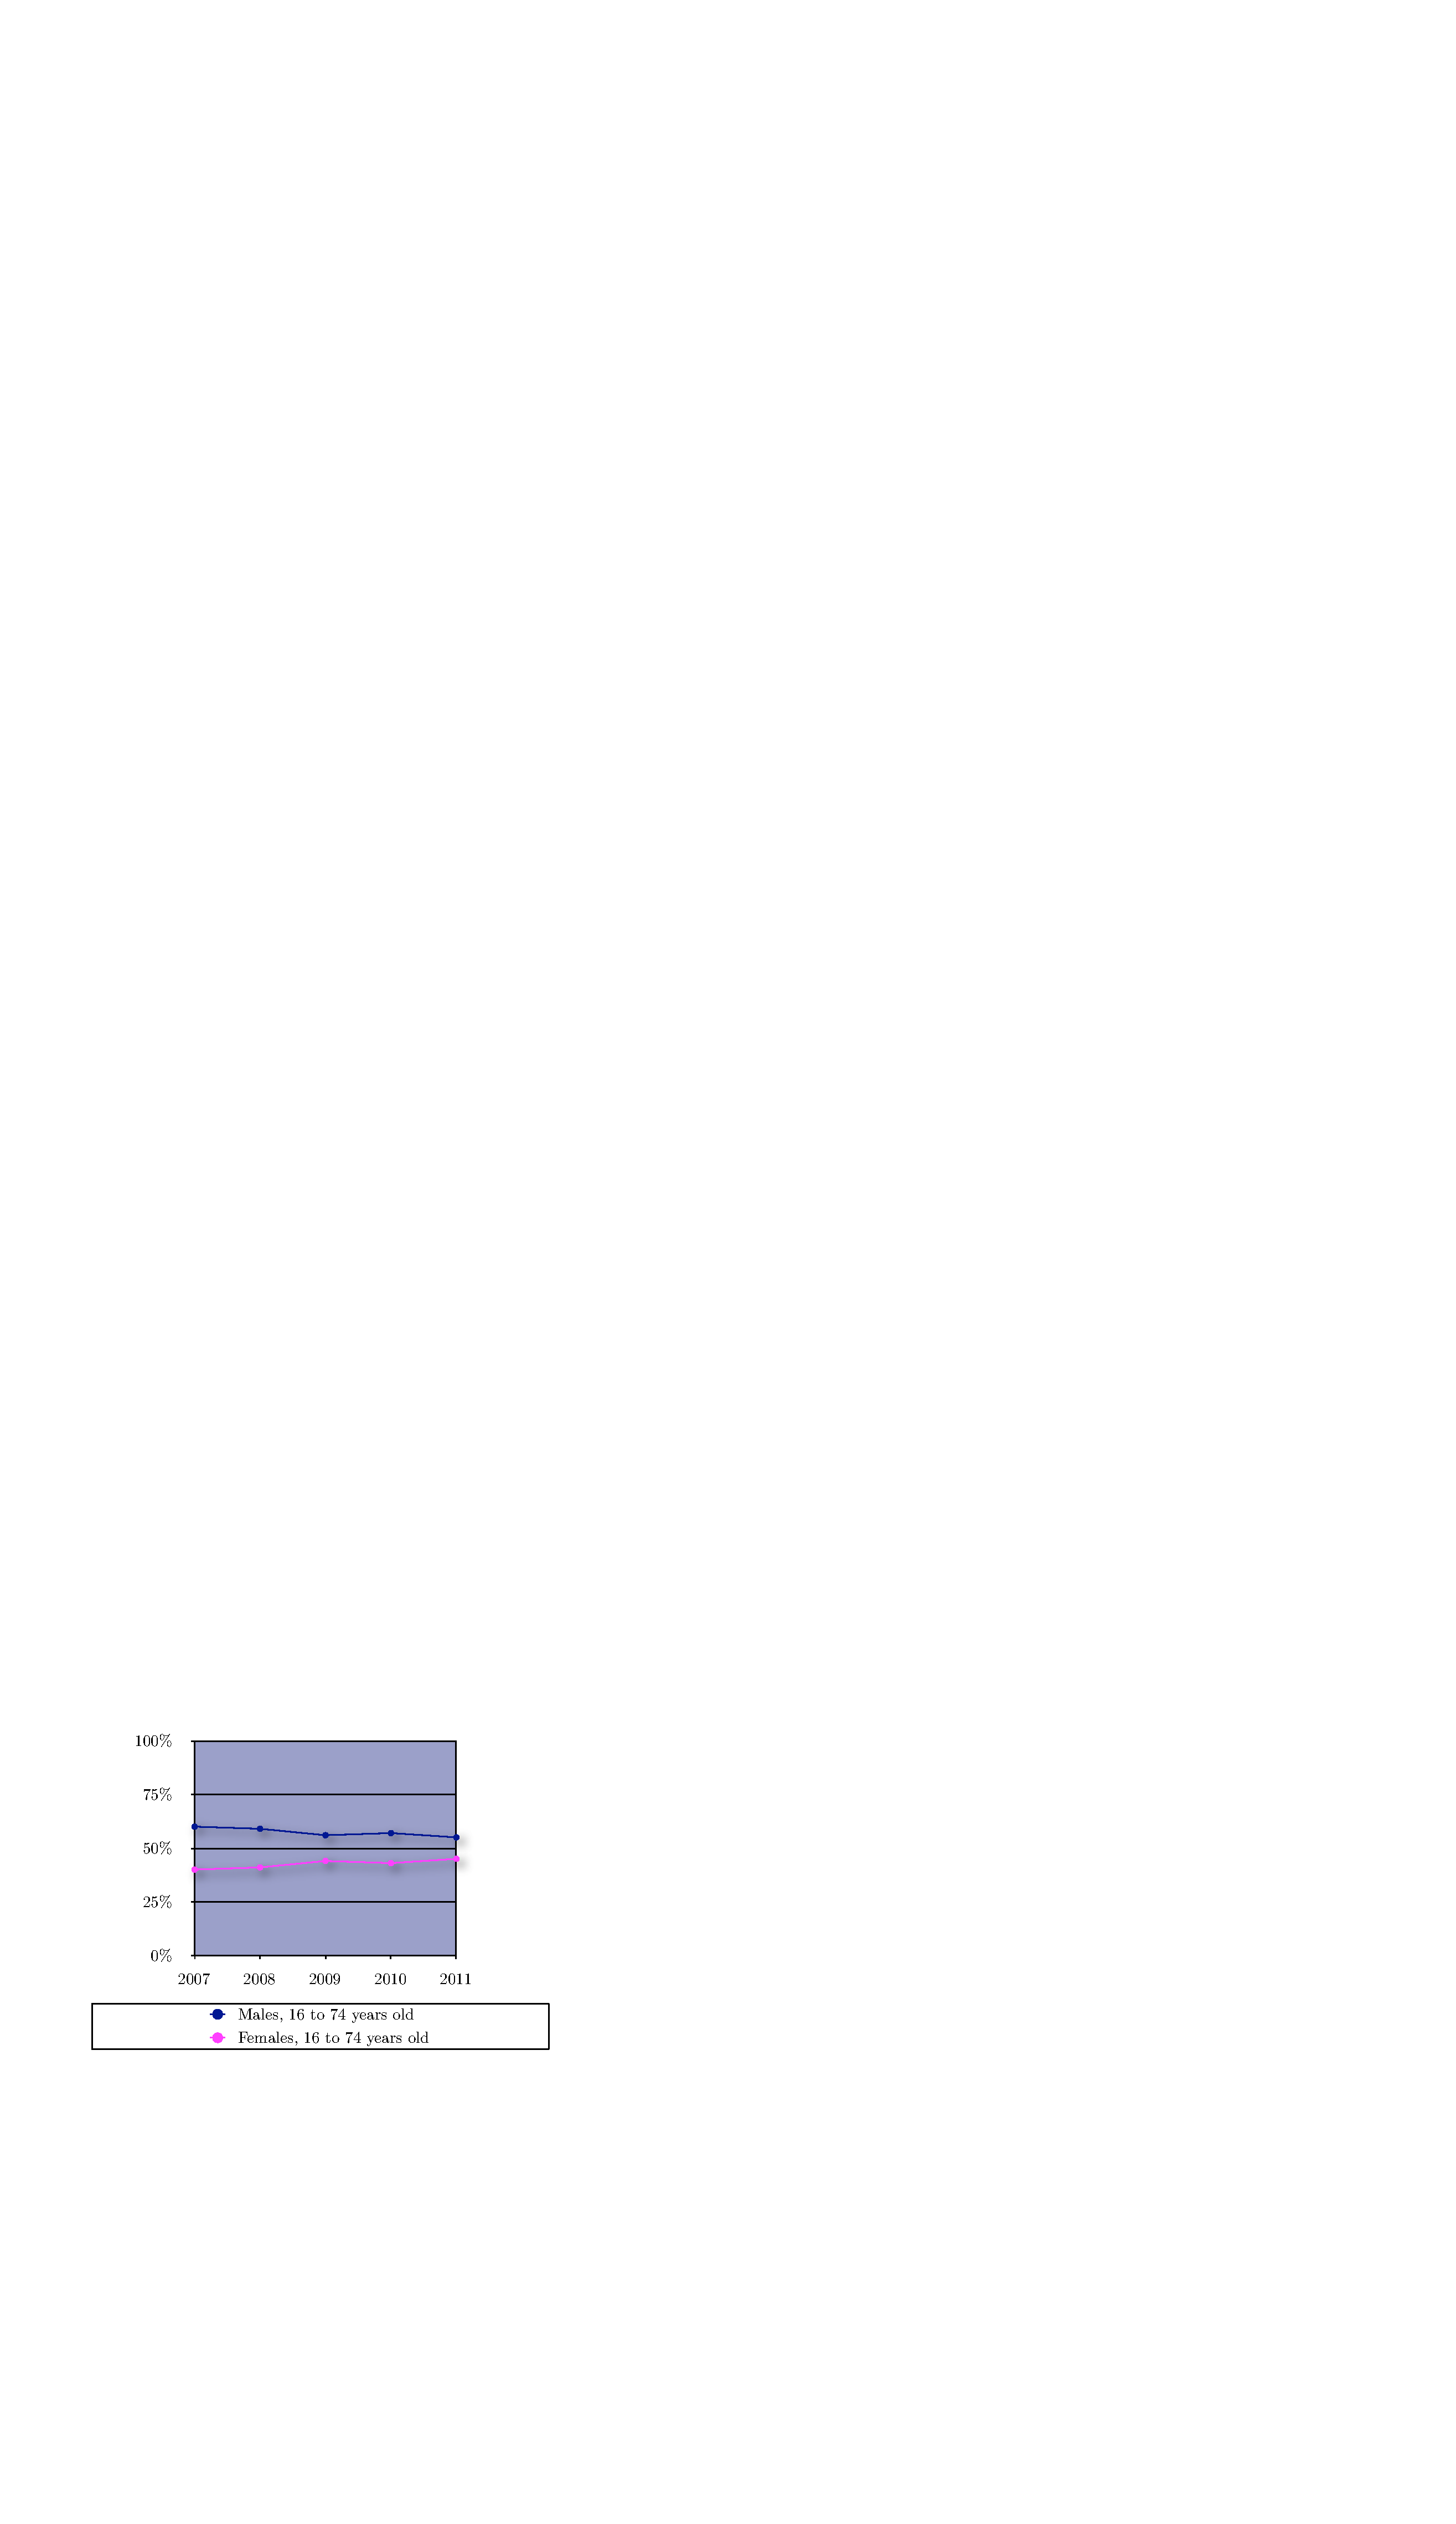
\includegraphics[width=.4\textwidth]{img/chart-males-females.pdf}
  %\label{fig:prototype-iteration3}
} \qquad
\subfloat[Third iteration of the prototype with a column-based and ``endless'' layout. Sections are placed beneath each other.]{
  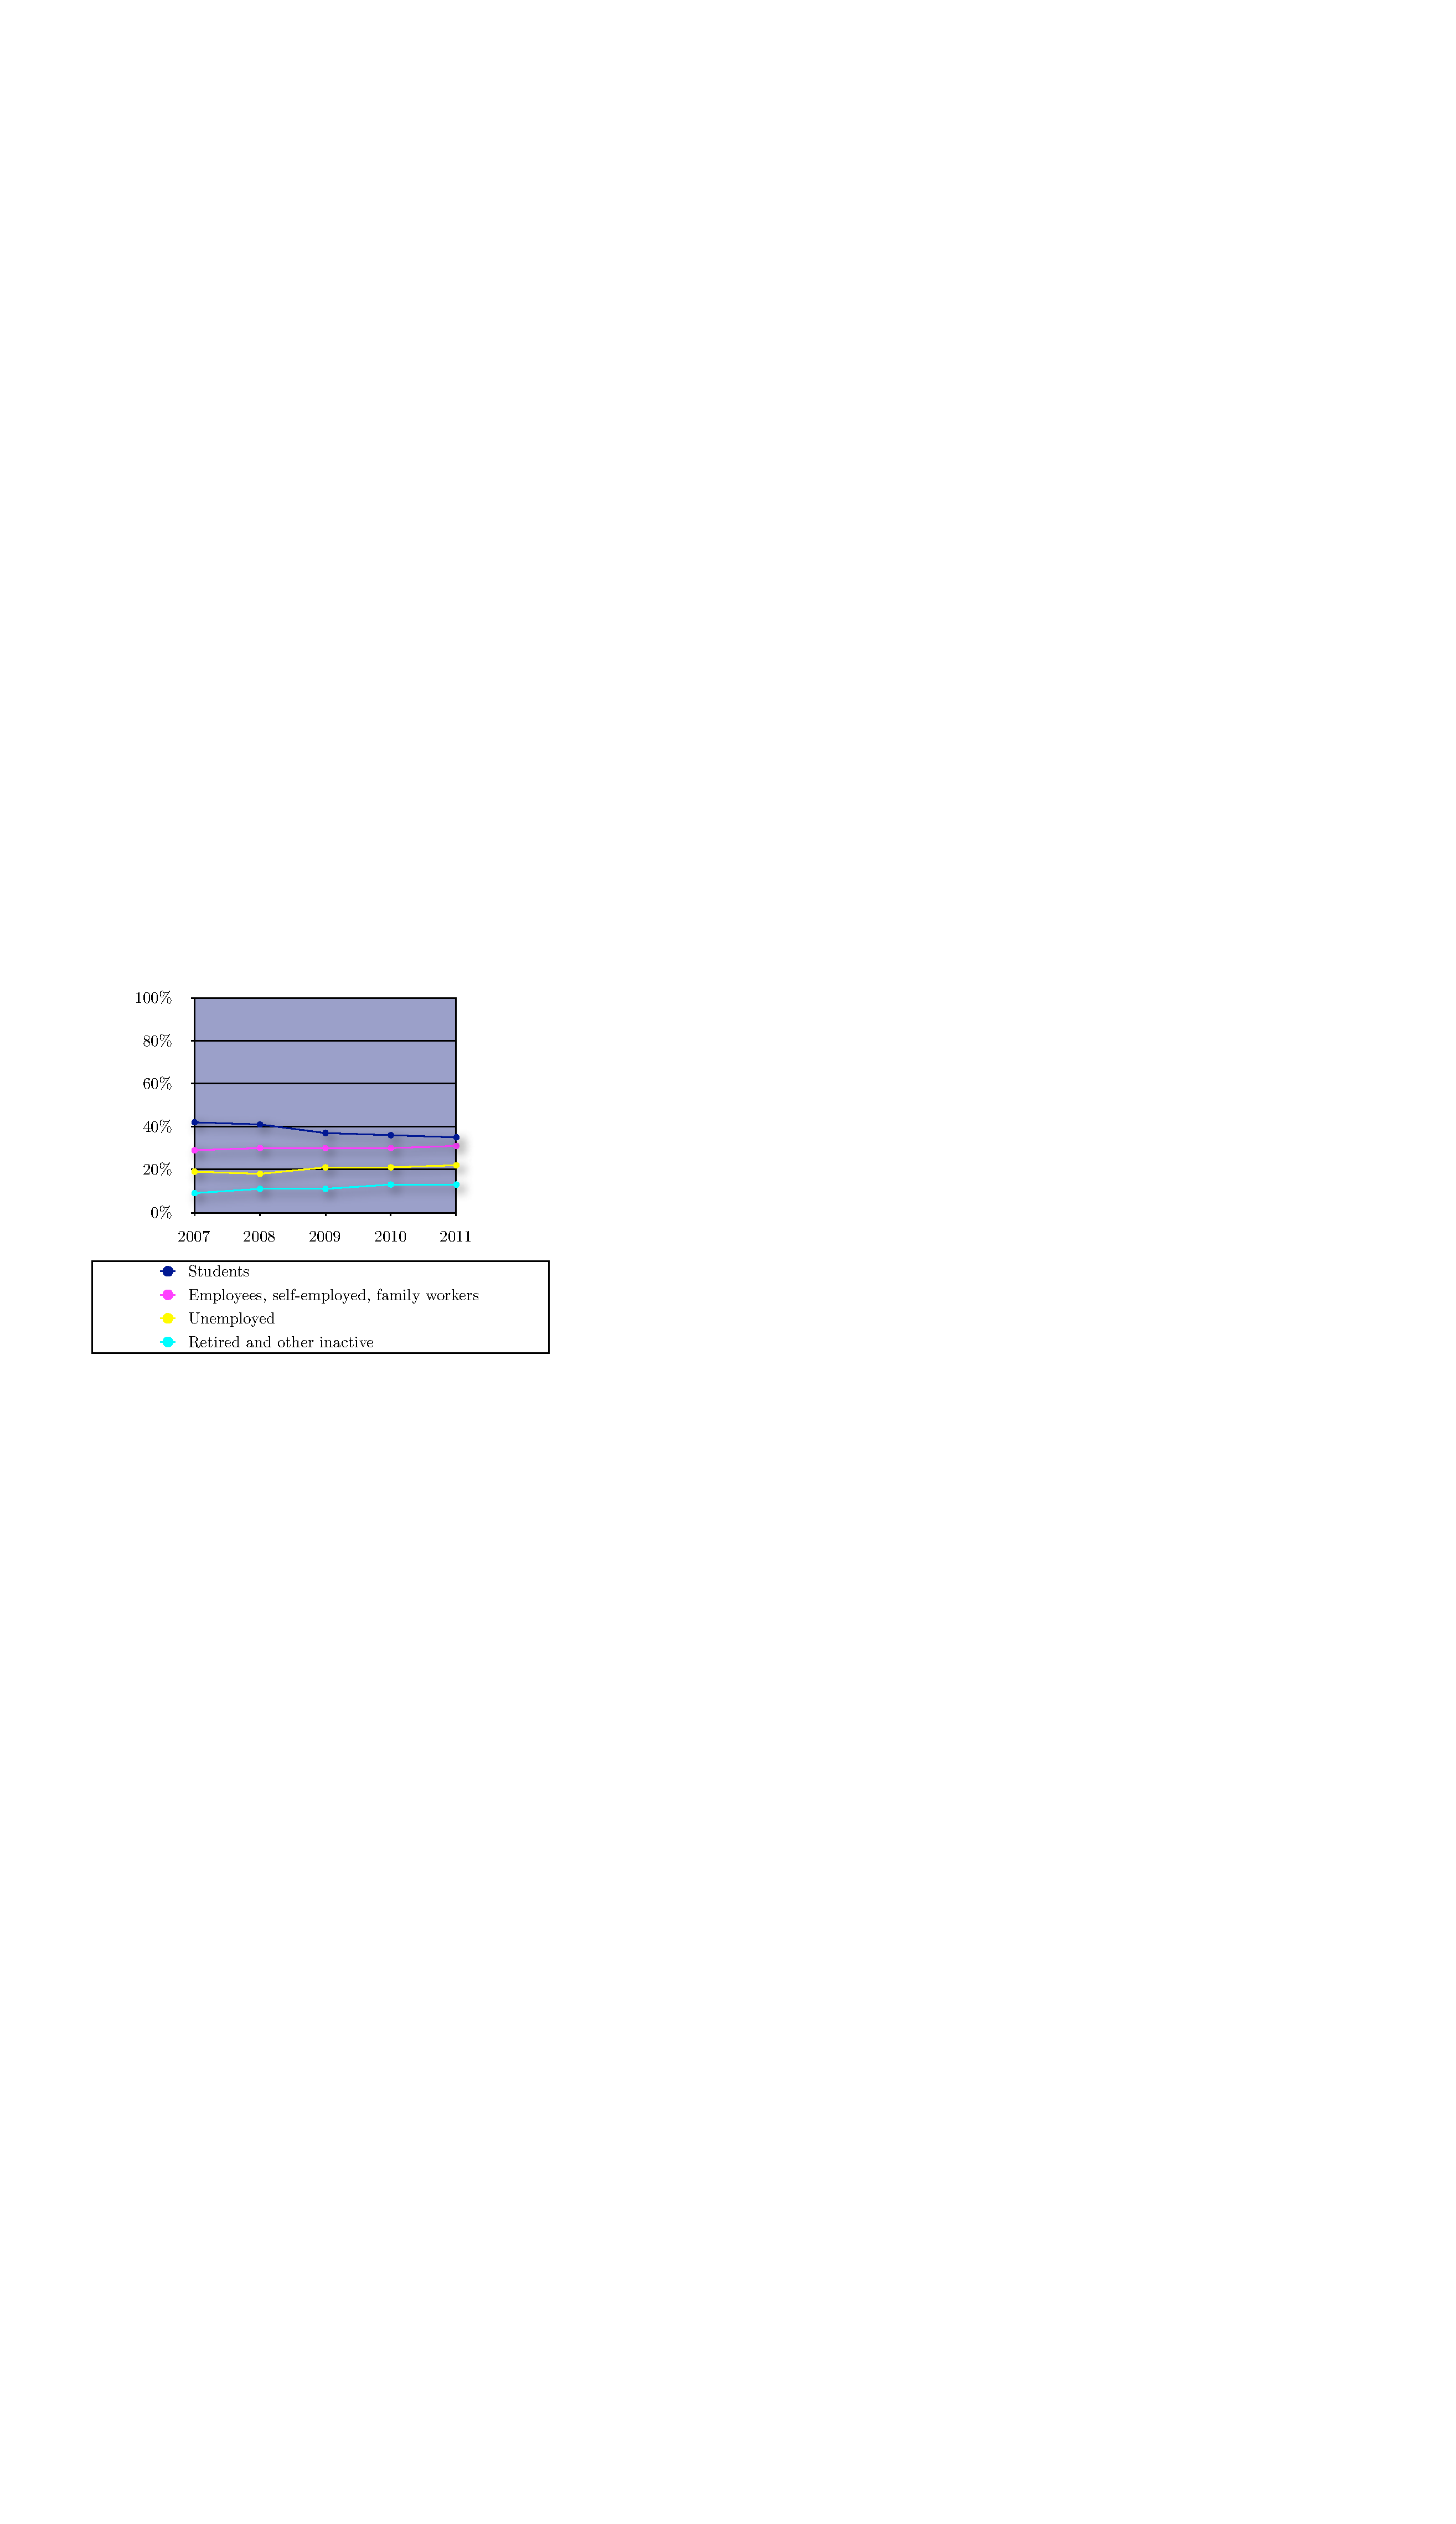
\includegraphics[width=.4\textwidth]{img/chart-occupation.pdf}
  %\label{fig:prototype-iteration4}
}
\caption{Eurostat: Individuals using the Internet for reading / downloading online newspapers / news magazines}
	\label{fig:charts-usergroups}
\end{figure}

In Figure~\ref{fig:charts-usergroups} is shown the basis for the division into the following user groups:
\begin{itemize}
	\item \url{student} 35\%, \url{employees self-employed family workers} 31\%, unemployed, retired or other inactive
	\item \url{high formal education} 50\%, medium formal education, no or low formal education
	\item \url{male} 55\%, female
	\item \url{16-24} 34\%, \url{25-54} 34\%, 55-64, 65-74
\end{itemize}

These provide the basis for the following personas.

\subsection{Thomas: student medium formal education male of age 21}
Thomas is 21 and a student at the Technical University of Denmark to be a bachelor of engineering in software. He is very interested in soccer and is therefore always updated on sports news. He reads about it online, newspapers and talks about it with friends. With big events he even likes to post it on Facebook. As a soon-to-be software engineer he has a natural thirst for news about technology, and he mainly reads these at home at the dormitory.
wired.com, newz.dk, engadget.com, facebook.com
computer, Samsung Galaxy Tab

\subsection{Laura: employed high formal education female of age 39}
Laura is 39 and is employed as a key account manager. She likes to be updated on strategies and economical status of rivalling companies. She is also very interested in politics and likes to discuss this subject with her friends. She reads economical news and likes to be updated on the run.
b.dk, borsen.dk, twitter.com
iPhone, iPad

\subsection{Marie: unemployed no or low formal education female of age 61}
Marie is 61 and a currently unemployed housekeeper. She spends her day looking for a job and taking care of her pet cat until her husband comes home. She mostly looks for the gossip sections or news about crime or big disasters. She also spends some time reading through the travelling guides as she dreams of going away with her husband.
ekstrabladet.dk, bt.dk, nyhederne.tv2.dk
computer, Lenovo IdeaPad A1

\subsection{Carl: retired or other inactive high formal education male of age 69}
Carl is a retired professor in psychology. He likes to discuss human behaviour and relation with his acquaintances and is very interested in cultural events. Therefore he often seeks the cultural sections and discussion fora to see what is going on. 
politiken.dk, aok.dk, dr.dk
computer, iPad

\section{Scenarios}
\subsection{Thomas}
Thomas comes home after a day at the study, picks up his tablet computer and opens Editor from the desktop. Editor opens and shows him the front page where all the headlines stories are displayed. The main story is about a new version of the Android OS that has been released today and presses it to read more. The story opens in a full window display with quality images to match the articles. He reads the first section and feels satisfied with the amount of information, but wants to share the information on Facebook, so he clicks share button and writes a comment and posts it on his Facebook wall. He closes the article and returns to the front page. He sees a top story below the main story about Mr. Mærsk Mc-Kinney Møller who has died. It is not a story that falls into his key interests, but as the news is big he is satisfied that he got informed about it. Thomas feels like reading more about technology so he opens the menu and chooses the ``Tech'' section he has installed in the application. The section opens with a head line and a page number to let him know where in his paper he has navigated to and finds an article about a new multicore CPU technology. He has never been interested in CPU technology before, but finds this technology interesting after reading about it, so he opens the application settings and types in keywords about the technology under his ``Tech'' section to keep him updated about it. He also adjusts the ratio between general and personal news, to be less personal as he feels like he needs to broaden his horizon a bit with respect to news. He closes the settings menu and Editor immediately starts updating the articles. Some new articles about CPU technology has been included amongst the articles in the ``Tech'' section after paging through the section and reading some of the most interesting articles he closes the application.

It could be nice if the key words of a story could be or is already highlighted, so he can click it and add it to his positive or negative list.

\subsection{Laura}
Laura is on the train on her way to a business meeting this morning and pulls out her tablet and sees she has one notification from Editor. She opens Editor to get updated on todays news. The front page is displayed and there are headlines from different top articles and a notification is shown in the corner. She presses the notification and the pages turns to show her the article, which opens in full screen. After reading it she wants to see todays headlines, so she presses the back button to return to the paper and presses the return to front page button and the paper turns pages to reach the front page. She scans the page to see if there is any big news about her rivalling companies. There is no breaking news, so she just turns the page to browse the content of todays paper. As she browses the ``Politics'' section of her paper she finds an article about the Prime Minister introducing a new bill about a toll ring around the capitol city. She chooses the article and it is shown in full screen. As she reaches the bottom of the article she sees the comments about it where her friends and most others are against it. She decides to join the discussion and posts a comment on the article wall. She also sees one of her friends has not commented on the article wall and decides to share the article with her as she thinks she would agree with her opinion. She presses the share button and chooses the Editor logo. A list of her friends is shown, some of them who has already read the article is greyed out, but the one she was looking for is not. So she chooses her and a notification is sent to her.

\subsection{Marie}
It is morning and Marie wants to check the news with her coffee in the couch, so she opens Editor from her tablet to get updated. The front page is displayed with a collection of stories as highlights of the content of the paper. It mainly contains stories about celebrities and a big disaster that has happened in japan, but there is also a story about a big political change, that she does not find interesting. So she goes to the settings menu and types in ``politics'' to add to her negative list. She also adjusts the personal/general news ratio to contain only personal news as she wants only news that is directed to her. She returns to the front page which is now free of political stories. Her newspaper contains many images and videos as she has set her graphical/textual content ratio more towards graphical content.

\subsection{Carl}
Sunday morning Carl wakes up, puts over the kettle to make a cup of coffee. While he waits for the water to boil he picks up his iPad and opens Editor to check the news. The front page opens with headlines from the different sections. There is a review article about a new show in the theatre. Carl presses the article and the system turns pages to the ``Cultural'' section of his newspaper and opens the article in full screen. Because the show gets good ratings he decides to order some tickets to him and his wife, which he does using the devices browser. After this he reopens Editor which opens in a display of the same article, as he left it. Carl pours his coffee and turn to the ``Funnies'' section. The section displays snippets of comics strips and some humorous and opinionated articles.

\section{Business Case}

\subsection{Need}
User value: personal quality and up-to-date stories enriched with quality images. This means that content providers should be chosen/verified. Same navigation as actual newspapers, but faster and with endless more content. Instantly up-to-date. Adaptive layout. Adjustable user profile.

\subsection{Approach}
personalised content + composition.

Constraint Programming: fast computation - good for optimal solutions, describes the generic solution in stead of how to solve or find it, very easy to tailor the problem definition of the solution and adjust it and even let users make the adjustments - transparency.

Content providers can get to know their readers preferences better and improve the provided content.

\subsection{Benefit Per Cost}
Revenue flow: Content providers are paid. Income from advertisers (scattered \cite[p. 6-7]{kristin_fredrik.pdf}) and users. Income from selling user behaviour patterns and targeted commercials.

\subsection{Competition}
FlipBoard, Wired magazine, Zite and app with actual editors affiliated.

\section{Requirements}
The above scenarios, user needs and business case led to the following requirements.

\subsection{Non-functional Requirements}
\begin{itemize}
	\item ``the clear overview of content, including a beginning and an end, the ease of use, typography and design'' \cite[p. 7]{FULLTEXT01.pdf}
	\item both general and personal news (collaborate filtering solves that some news are not received, but are universally interesting \cite{fulltext.pdf})
	\item familiarity in design from printed paper \cite[p. 7]{FULLTEXT01.pdf}
	\item Design and layout from printed newspaper \cite{hcii2005_1004.pdf}
	\item both images and videos - test
	\item a good ratio of graphical and textual - test
	\item front page should give a good overview of the content - test
	\item ``news valuation, e.g. positioning of lead story'' \cite[p. 7]{FULLTEXT01.pdf}
	\item  mobility \cite[p. 7]{FULLTEXT01.pdf}
	\item  continuous updates \cite[p. 7]{FULLTEXT01.pdf}
	\item ``easy and intuitive navigation'' \cite[p. 7]{FULLTEXT01.pdf}
	\item add video and sound \cite[p. 7]{FULLTEXT01.pdf}


	\item incorporate social community and social networks
	
	
\end{itemize}

\subsection{Functional Requirements}
\begin{itemize}
	\item ``open, turn pages, chose article, read and return'' \cite[p. 6]{FULLTEXT01.pdf}
	\item section headlines \cite[p. 6-7]{kristin_fredrik.pdf}
	\item article headlines
	\item article summaries / extracts \cite{fulltext.pdf}
	\item menu w. section headlines \cite[p. 8]{kristin_fredrik.pdf}
	\item page numbers \cite[p. 6-7]{kristin_fredrik.pdf}
	\item press ``like'' or key word based user profile (mark self or highlighted? right click to add): positive + negative list (keywords+categories \cite{10-1-1-19-5583}, \cite{fulltext.pdf} and \cite{gervasum2001ws.pdf})
	\item full screen display of article
	\item organise into personalised sections
	\item opens in front page view (summery of newspaper 8 articles) \cite[p. 8]{kristin_fredrik.pdf}
	\item adjust variables
	\item share directly (grey out the ones who have read it)
	\item comment
	\item see friends comments
	\item ``The presentation schema -- headline, abstract, and text, together with a relevance value with respect to the user profile -- rates the highest in terms of user satisfaction, and yet it is not the most frequent.'' \cite{Sections-categories-and-keywords-as-interest-specification-tools-for-personalised-news-services.pdf}
	\item  ability to search \cite[p. 7]{FULLTEXT01.pdf}
	\item Landscape + portrait \cite[p. 6-7]{kristin_fredrik.pdf}
	\item touch screen interaction \cite[p. 6-7]{kristin_fredrik.pdf}
	\item Functionality from online newspaper \cite{hcii2005_1004.pdf}
	\item Name of columnist \cite[p. 4]{gervasum2001ws.pdf}
	\item Transparency of implicit relevance feedback (see/modify current weights of categories) \cite[p. 7]{gervasum2001ws.pdf}
	\item dynamic short-term + static long-term user profile \cite{10-1-1-19-5583}, \cite{fulltext.pdf} and \cite{gervasum2001ws.pdf}
	\item relevance feedback \cite{10-1-1-19-5583}, \cite{fulltext.pdf} and \cite{gervasum2001ws.pdf}
\end{itemize} % Appendix A
%% Appendix X

\chapter{Appendix Title}

%----------------------------------------------------------------------------------------

% Content begins here % Appendix B - empty template

%----------------------------------------------------------------------------------------
%	POST-CONTENT THESIS PAGES
%----------------------------------------------------------------------------------------

\cleardoublepage% Bibliography

\label{app:bibliography} % Reference the bibliography elsewhere with \autoref{app:bibliography}

\manualmark
\markboth{\spacedlowsmallcaps{\bibname}}{\spacedlowsmallcaps{\bibname}} 
\refstepcounter{dummy}

\addtocontents{toc}{\protect\vspace{\beforebibskip}} % Place the bibliography slightly below the rest of the document content in the table of contents
\addcontentsline{toc}{chapter}{\tocEntry{\bibname}}

%\bibliographystyle{plainnat}
\bibliographystyle{named}

\bibliography{Bibliography} % Bibliography

%\cleardoublepage% Colophon (a brief description of publication or production notes relevant to the edition)

\pagestyle{empty}

\hfill

\vfill

\pdfbookmark[0]{Colophon}{colophon}

\section*{Colophon}

This document was typeset using the typographical look-and-feel \texttt{classicthesis} developed by Andr\'e Miede. The style was inspired by Robert Bringhurst's seminal book on typography ``\emph{The Elements of Typographic Style}''. \texttt{classicthesis} is available for both \LaTeX\ and \mLyX: 

\begin{center}
\url{http://code.google.com/p/classicthesis/}
\end{center}

\noindent Happy users of \texttt{classicthesis} usually send a real postcard to the author, a collection of postcards received so far is featured here: 

\begin{center}
\url{http://postcards.miede.de/}
\end{center}
 
\bigskip

\noindent\finalVersionString % Colophon

%\cleardoublepage% Declaration

\refstepcounter{dummy}
\pdfbookmark[0]{Declaration}{declaration} % Bookmark name visible in a PDF viewer

\chapter*{Declaration} % Declaration section text

\thispagestyle{empty}

Put your declaration here.
\bigskip
 
\noindent\textit{\myLocation, \myTime}

\smallskip

\begin{flushright}
\begin{tabular}{m{5cm}}
\\ \hline
\centering\myName, \today \\
\end{tabular}
\end{flushright}
 % Declaration

%----------------------------------------------------------------------------------------

\end{document}